%to have line numbers
%\RequirePackage{lineno}
\documentclass[10pt, letterpaper]{article}      
\usepackage[margin=.1cm,font=small,labelfont=bf]{caption}[2007/03/09]
%\usepackage{endnotes}
\usepackage{setspace}
\usepackage{longtable}                        
\usepackage{anysize}                          
%\bibpunct{(}{)}{,}{a}{,}{,}                   
%\bibpunct{(}{)}{,}{a}{}{,}                   
\usepackage{amsmath}
\usepackage[pdftex]{graphicx}  %[pdftex]git latex doesn't like it             
\usepackage{epstopdf}
\usepackage{hyperref}                             % For creating hyperlinks in cross references


% \usepackage[margins]{trackchanges}

% \note[editor]{The note}
% \annote[editor]{Text to annotate}{The note}
%    \add[editor]{Text to add}
% \remove[editor]{Text to remove}
% \change[editor]{Text to remove}{Text to add}



\marginsize{1cm}{1cm}{.5cm}{.5cm}%{left}{right}{top}{bottom}   
					          % Helps LaTeX put figures where YOU want
 \renewcommand{\topfraction}{1}	                  % 90% of page top can be a float
 \renewcommand{\bottomfraction}{1}	          % 90% of page bottom can be a float
 \renewcommand{\textfraction}{0.0}	          % only 10% of page must to be text

 \usepackage{float}                               %latex will not complain to include float after float

\usepackage[table]{xcolor}                        %for table shading
\definecolor{gray90}{gray}{0.90}
\definecolor{orange}{RGB}{255,128,0}

\renewcommand\arraystretch{.9}                    %for spacing of arrays like tabular

\newenvironment{ig}[1]{
\begin{center}
 %\includegraphics[height=5.0in]{#1} 
 \includegraphics[height=3.3in]{#1}
\end{center}}

 \newcommand{\cc}[1]{
\hspace{-.13in}$\bullet$\marginpar{\begin{spacing}{.6}\begin{footnotesize}{#1}\end{footnotesize}\end{spacing}}
\hspace{-.13in} }

\usepackage{datetime}


%\usepackage[latin1]{inputenc} %git latex compiler doesn't likeit
\usepackage{tikz}
\usetikzlibrary{shapes,arrows,backgrounds}


%\usepackage{color}					% For creating coloured text and background
%\usepackage{float}
\usepackage{subfig}                                     % for combined figures

\renewcommand{\ss}[1]{{\colorbox{blue}{\bf \color{white}{#1}}}}
\newcommand{\ee}[1]{\endnote{\vspace{-.10in}\begin{spacing}{1.0}{\normalsize #1}\end{spacing}\vspace{.20in}}}




\usepackage{sectsty}
\allsectionsfont{\normalfont\sffamily}



\usepackage{sectsty}
\allsectionsfont{\normalfont\sffamily}
%\usepackage[margins]{trackchanges}

\renewcommand\familydefault{\sfdefault}

\usepackage{verbatim}
\usepackage{rotating}
\usepackage{catchfilebetweentags}
%-------------------- END extra options -----------------------------------------
\date{Draft: {}\today}
\title{
%  The Paradox of Energy Consumption and Happiness Across Countries
%Presonal 
Energy Use And Happiness\footnote{Author Contributions: A.O.K and M.A designed
  research. A.O.K. performed research. A.O.K. analyzed data. A.O.K. and
  M.A. wrote the paper.  % Micah: Add author contribution statements. See: http://www.nature.com/news/publishing-credit-where-credit-is-due-1.15033
}
}
\author{
Adam Okulicz-Kozaryn\thanks{EMAIL: adam.okulicz.kozaryn@gmail.com
  \hfill I thank XXX.  All mistakes are mine.} \\
{\small Rutgers - Camden}\\
Micah Altman\thanks{EMAIL: ???
  \hfill I ???} \\
{\small MIT}
}

\begin{document}

%%\setpagewiselinenumbers
%\modulolinenumbers[1]
%\linenumbers

\bibliographystyle{/home/aok/papers/root/tex/pnas2011.bst}
\maketitle
\vspace{-.4in}
\begin{center}

\end{center}

\begin{abstract}
\noindent  

% 4/13
% TODO 
%
% - Make sure paper actually does these things... aok:it does!

It is widely claimed that there is a substantial trade-off between energy consumption and wellbeing. 
Despite technological advances, the Earth per capita energy use continues to grow.
The environmental consequences of high rates of energy consumption are well known:
resource depletion and pollution. Is this avoidable?

We study the relationship between energy consumption and happiness across four decades, and across multiple levels of geography.  Surprisingly, we find that received wisdom is false -- for counties, states and nations, energy consumption is neither necessary for well-being, nor linked directly to it. 

%aok: i though we focus now too much on en intensity, and this is just one panel
%of one graph; the overall argument was about energy use in general

% We find instead that national well-being is strongly associated with the energy intensity of GDP. Although not a necessary condition for well-being, countries that efficiently convert energy to economic wealth, may benefit from increased energy use. 

% We lay out the possible causal explanations for differences in the energy intensity of GDP. Based on this we summarize the potential implications for designing policies that yield both high well-being and modest energy use. 
\end{abstract}


\vspace{.15in} 
\noindent{\sc keywords:  energy use,  energy intensity of economy, sustainability, wellbeing,  happiness, Subjective Well-Being (SWB)}
%\vspace{-.25in} 

\begin{spacing}{1.4}
\rowcolors{1}{white}{gray90}

%  \ExecuteMetaData[../out/tex]{ginipov}

% \begin{figure}[H]
%  \includegraphics[height=3in]{../out/gov_res_trust.pdf}\centering\label{gov_res_trust}
% \caption{woo}
% \end{figure}

% Micah: 
%  Start with the strongest introduction we can possibly support. If we can't rigously support it with the data and analysis, we'll weaken it... but this is the goal. 
%  -- begin intro -- 

Environmental consequences of human consumption are the largest challenges to
science and society today. Energy consumption is a key component--the climate problem is mostly an energy problem \cite{mackay08}. Despite
technological advances, the Earth per capita energy use has increased about 40\%
over past 40 years and it continues to grow. % (1890-1336)/1336
Most energy consumption both pollutes and  depletes natural resources
\cite{arrow04, soytas07}. %recent us: http://www.eia.gov/tools/faqs/faq.cfm?id=427&t=3 and
                          %for world even worst http://www.google.com/url?sa=t&rct=j&q=&esrc=s&source=web&cd=7&sqi=2&ved=0CDwQFjAG&url=http%3A%2F%2Fwww.iea.org%2Fpublications%2Ffreepublications%2Fpublication%2Fkeyworld2014.pdf&ei=uPMVVYaSM8OhgwSjqIKIAQ&usg=AFQjCNFX92MbI8lsvnDKqHCZqqoBnSMtSQ&sig2=NZpGqw3hDWdm3xcxvQyizA&bvm=bv.89381419,d.eXY&cad=rja  
 Energy consumption has, of course, many benefits as well.
 % TODO check these
% references if they are really to the point ! and possibly add some from goog
% drive folder
% Energy use and pollution are highly correlated, but they are not the same,  and
 The question remains about the net effect, how energy use affects human wellbeing.
 % we will differentiate between various types of energy use.  
We use a happiness yardstick
to evaluate benefits and problems of energy use. Traditionally, Gross Domestic
Product and its adjustments--per capita and purchasing power parity--have been used to evaluate development. Human Development Index (HDI)
added life expectancy and education, but more recently a co-inventor of HDI,
Amartya Sen, has proposed happiness as better measure of overall development or
progress 
\cite{stiglitz09al}. 

% importantly there is spatail mismatch in resource demand and supply--notably
% china need a lot and has few; opec countries have oil; etc etc
%for instance recent emissions cap deal between US and China has largely to do
%with enrgy use e.g. http://mobile.nytimes.com/2014/11/13/opinion/climate-change-breakthrough-in-beijing.html?_r=0
It is universally acknowledged that there is a fundamental tradeoff between
societal energy preservation and individual self-interest. Substantially reducing
energy consumption requires individual sacrifices. If we reduce consumption, our wellbeing will
suffer \cite{kenny_businessweek_aug_29_14, gordon_wsj_may_29_14, carter_pbs_apr_18_77,smil05}. 
%COPIED FROM http://www.sciencedirect.com/science/article/pii/S0301421511001042
% The remarkable improvements in quality of life that occurred during the industrialization of Europe, North America and Japan in the 19th and early 20th centuries were caused, in large part, by the invention and adoption of energy intensive technologies (Smil, 2005). Coal was used to fuel steam engines, petroleum fed internal combustion engines, and all the fossil fuels plus falling water turned electrical generators.

%also, the point is that there is more popular wisdom instead! we know little scientifacally!hence our paper!

% and there is a Lancet series; but they did with health what we do with
% happiness:energy helps with health but also destroys it:
% http://www.sciencedirect.com/science/article/pii/S0140673607612537
% http://www.sciencedirect.com/science/article/pii/S0140673607612586
% http://www.sciencedirect.com/science/article/pii/S0140673607612525
% http://www.sciencedirect.com/science/article/pii/S0140673607612598
% http://www.sciencedirect.com/science/article/pii/S0140673607612550


% A very fundamental question is how to achieve both happiness and
% sustainability--it is difficult because there appears to be a tradeoff.
% Fundamentally,
%  the ultimate goal of increased energy consumption is human
%  happiness--if there is no relationship between the two, then we can
%  consume less and stay happy.

In this paper, we find that this universal assumption is wrong.  By combining
data on energy consumption and happiness we find that the
relationship is weak at best. % , with exception of poor countries, where more energy is% nneded for greater happiness.
 People in areas consuming more energy are not happier.
This finding is robust across time, and multiple levels of spatial aggregation--it applies to patterns of energy consumption  at the local, national, and global scale.  


% -- end intro -- 

%Energy consumption matters.% beyond happiness
 Energy is a strategic
resource. Countries wage wars about energy sources  and much of politics is
driven by energy. Many countries' whole economies depend on energy exports, for instance OPEC countries. Many other countries rely heavily on energy production
and some use it as a political tool, for instance, Russia.   
Virtually all countries  always seek to obtain more energy sources. A recent example is so called
fracking. Yet, we need to consume less. There are at least two
obvious reasons--most of energy consumed  is non-renewable and will stay
that way for some time\cite{mackay08}--most energy comes from
fossil fuels, which will run out. %MAYBE be specific give numbers
Second, energy consumption results in pollution and pollution harms not only
 environment and other species, but also  humans \cite{mackerron09,gandelman12,ferreira13}, the beneficiaries of energy
consumption, and thus pollution potentially cancels out the benefits of energy
consumption. 
 
A recent report by
Intergovernmental Panel on Climate Change is alarming 
(\url{http://www.ipcc.ch/}). % very important body; another pnas citing it
                             % already in title http://www.pnas.org/content/104/24/10288.full
Indeed, a threat is serious enough that
claims for not growing the economy anymore or even ``degrowing'' it
appear reasonable \cite{kallis11, kallis12}. % \footnote{Although it is not
  % immediately obvious what is the best strategy to achieve greater
  % sustainability--degrowth \cite{kallis11} or simply public policy
  % \cite{bergh11}--for more discussion see \cite{daly13,kallis12}.}
At very
least curbing consumption is a reasonable course of action. Some argue reduction as high
as by factor of 10 in affluent societies \cite{pretty13}. This,
of course, begs a question, what would happen to our wellbeing?
 Again, a common % or received
wisdom is that there is a tradeoff between happiness and
energy use--we need to consume energy in order to achieve greater
happiness. One could even say, that the very end goal (usually implicit)
of energy consumption is wellbeing or happiness.  % This is
% true in buivaraite case--the richer areas are happier.
%  We argue here that it is not necassarily so, only after taking into account
%  income at country level % and few other variables at state or county levels,
%  the relationship between energy consymptiona nd happiness disappears.
%
% its striking 2 fold or more differences between states like nj and tx and only a
% small fracton of that is due to climate most due to consumption arguably
% wateful/conspicous--calculate how mich explained by climate! give number
Arguably a major, if not key, factor prohibiting us from conservation and
sustainability is fear of loss in wellbeing--we argue here that such loss, if
any,  will
not be substantial. Indeed, our results suggest that curbing energy consumption that results
in pollution, i.e. most of today's energy use, will not affect adversely our
happiness.  % There is anectodal evidence pointing to the fact that humans can
% live happily without much energy--among Amish, African Maasai, and Greenlandic
% Inughuit, most people are above neutral in well-being. \textbf{TODO cite!}

At the country level, we show that the lower the energy consumption, given development
level, the happier the country.  Across US states and California counties,
energy consumption and happiness have a nil relationship. 
% it would be another reason for energy
% conservation.
Likewise, the over time changes in energy use are almost unrelated to changes in
 happiness across US Census regions. 
These are important findings  because many assume that energy consumption makes us
happy--this is presumably why we keep on consuming ever more energy and are
reluctant to curtail this consumption. % At the same time, there are important
% reasons to curtail the consumption.
With this correlational study we aim to bring the relationship between energy
use and wellbeing to wider audience, and encourage more research in this area. 

% Germany plans for renewable energy
% http://www.nytimes.com/2014/12/01/business/energy-environment/plan-outlines-low-carbon-future-for-germany-energy.html

\section*{\large \bf Results}

% Micah: This needs to be reorganized. 

% In my view the primary goal of this section is to answer this question:
%  *** Which choices do individuals make, that have a large negative effect on the environment, and which do not make the individuals, their community, or society better off?  ***
% We aim to provide the best scientifically and empirically supported answer possible, that does not require collecting new primary data. 


% AOK: another paper !
% this is interesting, probably more interesting than what we have so far, the
% problem is that we did not really test for that; now i was actually surprised
% that there are  data by census or climate
% regions (9 of them): 
% http://www.eia.gov/consumption/residential/data/2009/index.cfm?view=consumption
% and we have happiness there too: but you are asking a grand question; and the
% data we have just breaks down energy use in a big region estimating how much is
% used for cooling, heating, lights, etc etc--but there are a function of climate,
% culture and other collective stuff; for your question we would need person-level
% data and there are some (PSID for instance), but that's a different paper...

% what we have done so far is that there is not much happiness from energy use;
% probably much less than expected...

% and then we can say that given that we can cut energy consumptin and stay happy

% so yes in a sense we do answe your question--it is just not ``which choices''
% buty specifically less energy in general

% I suggest the following organization
%  1. Provide an easy to interpret figure showing happiness vs. energy consumption at the global level (nations), for a single time period. This should illustrate the general weakness of the relationship between happiness and energy consumption without controlling for anything. Discuss the substantive size of the raw - uncontrolled correlation
% 2. Now discuss the details of the measures. explain that (a) the energy
% consumption measures include only those that are under personal control, 

% AOK: all residential is personal control; but affected by climate etc--hence we
% have controls

% and (b) have a substantial effect on environment. Cite the literature as appropriate

% AOK ok, cool will trhow in lit here

% 3. Show that this relationship is durable -- introduce time-series data to show that this holds over significant time-scales

%AOK:by relationship i guess you mean happiness-energy use; but happiness is
%mostly flat over time; same energy use: in the rich countries mostly flat or
%increaing a little; in developing it increases;so won't be much there

% 4. Show that this relationship is not an accident of scale. Drill down to states, then counties within california, and show the relationship holds
% 5. Now discuss other possible explanations for these patterns (a) use these explanations to suggest convariates/confounders (b) show the results of controlling visually first, or with a simple table, (c) use a statistical model to ensure that the visual impressions are not misleading

\textbf{Global patterns.} We start by examining the relationship between energy use and well-being across the world, at the level of individual countries.  % --there is not much variation in happiness over
% time, and energy consumption in developed areas is quite flat, too. 
We use happiness data from World Values Survey
(WVS, \url{http://www.worldvaluessurvey.org}).  Happiness is measured with answers to
"All things considered, how satisfied are you with your life as a whole these
days?" on scale from 1="dissatisfied" to 10="satisfied."
The measure of total energy  consumption comes from the World Bank
(\url{http://data.worldbank.org/indicator}). Data are plotted in figure \ref{couWvsLsEnePerGdp2}.
 %we use total and not residential
                                %electricity because across countries it is
                                %about energy intensive technologies of the
                                %whole economy, type of economy...,  not just households that
                                %determine QOL and happiness of people; within
                                %countries these ar emore or less constant and
                                %hence we can focus more on personal consumption
% 
%
% may also say that there are severalfold diff not only in income but also in ene
The basis for the received wisdom that increasing well-being requires increased energy consumptions is illustrated by the figure on the left: Across countries, there is a clear positive association between greater energy use, and greater well being.

Even this simple figure reveals some puzzles: Although the relationship between
well-being generally increases with energy consumption -- the variance across
countries is tremendous. Further, some countries with high energy use, such as
Russia (RUS)  and Estonia (EST) have low overall well being, the highest energy
users do are not the most well-off overall, and many countries such as Colombia
(COL), Guatemala (GTM) and Mexico (MEX) are able to reach the highest level of subjective well-being while maintaining very low energy use. What could account for this? 

% 4/13
% TODO 
%
% Fig 1a - graphical emphasize high well-being/low energy countries
% Fig 1a - do we really believe Mex, Guatemal and Colombia have higher well-being -- seems like WVS may be incompletely
%		   measuring this

Moreover, the two countries that most strongly contribute to the positive relationship between energy consumption and happiness are the highly-developed Nordic countries -- which have both unusually high energy use and happiness. Prior work shows that higher development is related to greater quality of life and well-being \cite{mazur11}: Could the relationship between energy use and well-being be driven by characteristics of development unrelated to overall energy consumption?

% 4/13
% TODO 
%
% Is the attribution to Nordic countries correct?
% Can we answer the question, at least partially?
% sure there is a lot of other things predicting happiness! Scandinavia uses a
% lot of energy because it is freezing there, and it is arguably v happy due to
% great governance, welfare, nature, low density etc etc

Most surprisingly,  we find that when we measure energy as as a function of economic efficiency, the relationship reverses.  This is shown in the second panel, which displays, on the x axis, the energy intensity of the gross domestic product (energy/GDP). This reveals that countries that  consume less energy per unit of wealth are better off. 

In a descriptive sense, high energy intensity indicates that a country requires
a high cost to convert energy into GDP. Another way to put this is that some
countries are more efficient (in the economic, not technical sense) at
converting energy into wealth. We discuss causal explanations in discussion section.

%was thinking about how to neutralize too happy COL and few others, but it is
%what it is,may explain this a bit in text perhaps--e.g. see http://www.huffingtonpost.com/2013/01/17/reasons-colombia-happiest-country_n_2490813.html
In figure \ref{couWvsLsEnePerGdp2} most countries conform to the predicted pattern. 
 For instance,  the Netherlands (NLD) is rich,  energy efficient and happy. But
 there are also some outliers, for instance,  Colombia (COL) is  happy and energy
 efficient,  but poor.  
In general, Latin America poses a puzzle for happiness researchers. Latinos are
relatively poor and yet quite happy. They also use very little  energy and have similar energy intensity of GDP to that of the  US. Notably, all Latin
 American countries cluster at the top left in the
first panel.  Great happiness is possible using little  energy. East European
post-Soviet countries, on the other hand, cluster at the bottom and some at the
left. Some countries are relatively unhappy despite low energy intensity of GDP,
such as Albania (ALB). Some countries, on the other hand, are relatively happy
despite low energy efficiency such as Nigeria (NGA) and Kyrgyzstan (KGZ).    
% also see http://www.ritholtz.com/blog/2010/06/oil-consumption-around-the-world/ 
%TODO fix country codes to 2 letters
\begin{figure}[H]
 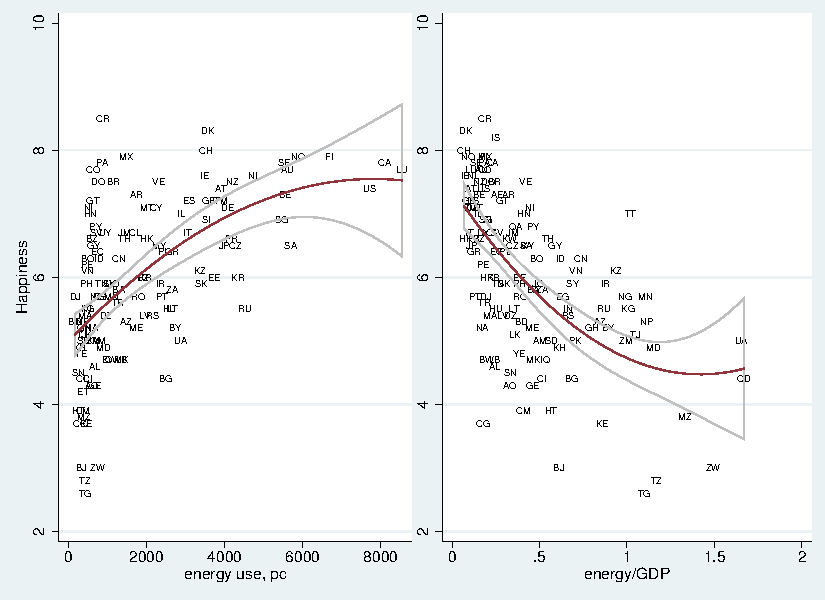
\includegraphics[width=6in]{graphsAndTables/couWdhEneGdp.pdf}\centering \caption{Happiness against GDP,  and energy intensity of GDP. Quadratic fit shown with 95\% confidence intervals. Happiness data come from World Database of Happiness and is measured on scale from 0="dissatisfied" to 10="satisfied. Data come from multiple sources and were averaged for 2000-2009 period. For details see \url{http://www1.eur.nl/fsw/happiness/hap_nat/nat_fp.php?mode=8}.  Energy use refers to use of primary energy before transformation to other end-use fuels, which is equal to indigenous production plus imports and stock changes, minus exports and fuels supplied to ships and aircraft engaged in international transport. % For average electricity consumption per electrified household, which shows a similar picture, see figure \ref{couWvsLsEleHHgdp} in supplementary material.
For graphs using happy life years as a dependent variable see graph \ref{hly} in
supplementary materials.  Note: Country codes are in table \ref{ls} in supplementary material. Energy and GDP data were also averaged over 2000-2009 period. In addition several outliers were dropped: countries with ebnergy use above 10,000: United Arab Emirate Iceland Kuwait Qatar Trinidad and Tobago; and countries with energy intensity higher than 2: Ethiopia Turkmenistan Uzbekistan}\label{couWvsLsEnePerGdp2} 
\end{figure}
% \begin{figure}[H]
%  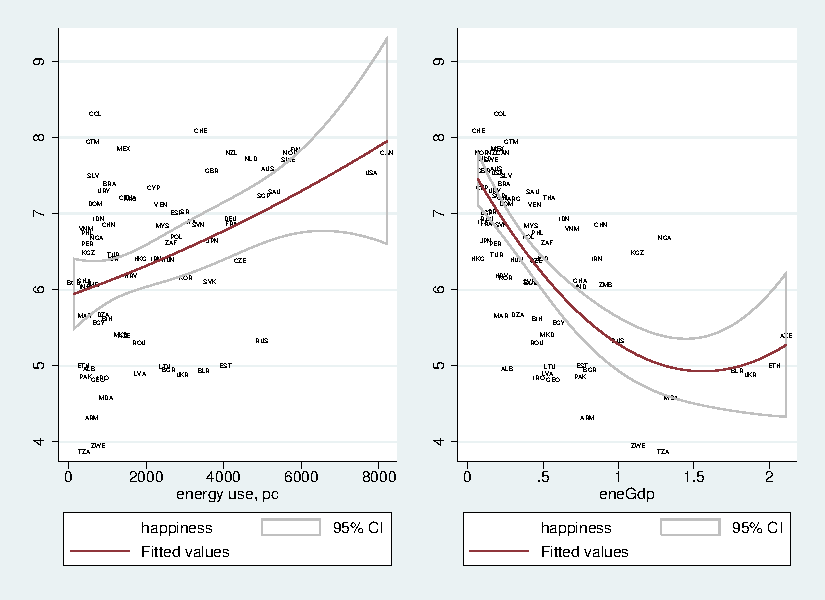
\includegraphics[width=6in]{graphsAndTables/couWvsLsEnePerGdp2.pdf}\centering \caption{Happiness
%    against GDP, total energy use, and energy intensity of GDP. Quadratic fit
%    shown with 95\% confidence intervals. Happiness is measured with "All things considered, how satisfied are you with your life as a whole these days?" on scale from 1="dissatisfied" to 10="satisfied." Energy use refers to use of primary energy before transformation to other end-use fuels, which is equal to indigenous production plus imports and stock changes, minus exports and fuels supplied to ships and aircraft engaged in international transport. For average electricity consumption per electrified household, which shows a similar picture, see figure \ref{couWvsLsEleHHgdp} in supplementary material.  Note: Country codes are in table \ref{ls} in supplementary material. We use a cumulative file covering first four waves, 1981-2007. If country was observed in more than one year, data were averaged.}\label{couWvsLsEnePerGdp2} %couWvsLsEnePerGdp2 doesn't have gdp only; couWvsLsEnePerGdp2 adds gdp as first panel
% \end{figure}


% In poor countries more income and sometimes more energy may be beneficial to human
%  wellbeing. In rich countries, on the other hand,  it is likely that not only we do not need
% more energy, but also, arguably we should consume less energy \cite{mazur74}. There are even
% calls to stop growing income in rich countries or even degrow it
% \cite{kallis11,kallis12,bergh11}.
We  focus now on the US in an effort to answer
an old question of whether more energy is needed to increase wellbeing if there
is already a great deal of energy being consumed \cite{mazur74}. The US is among
countries using most energy per capita.
% Also, we focus
% now on electricity consumption because it is representative of modern
% energy %niu13 
% and it is growing fast. %winfrey13 p7
% electricity for CA only--can add this explaation + lack of total energy use i
% guess if reviewers compalin about electricity in california! 
%
 We zoom in on US states and California counties.

State and county level happiness data come from Behavioral Risk Factor
Surveillance System (BRFSS) using a very similar question to WVS ``In general,
how satisfied are you with your life?'' on scale 
from 1=''very dissatisfied'' to 4=''very satisfied.'' State energy use data come from
U.S. Energy Information Administration and is measured as  total energy
consumption per capita in the residential sector.  
California's  residential electricity consumption per capita come from 
Energy Consumption Data Management System
(\url{http://www.ecdms.energy.ca.gov/elecbycounty.aspx}). Results are shown in
figure \ref{stateCaPAP}. Energy-hungry states (with possible exception of transportation sector) are not happier% --this is just another argument for energy conservation
. There are two outliers, Hawaii and California consuming much less energy in
the residential sector than others. 

We zoom in on California counties in
second panel of the same figure. Like among states, there is a great deal of variation in energy
use across California counties, and also the 
relationship with happiness is nil. 
% So California consumes only about half of the energy consumed by an average
% state.  also see http://www.skepticalscience.com/print.php?n=1365
We have also experimented with energy intensity of
GDP as we did earlier across countries, but in case of the US subregions the results are
similar. %supplemnetart material picture XXX

%MAYBE can make it flatter as fig 1 so that subgraphs are square
\begin{figure}[H]
 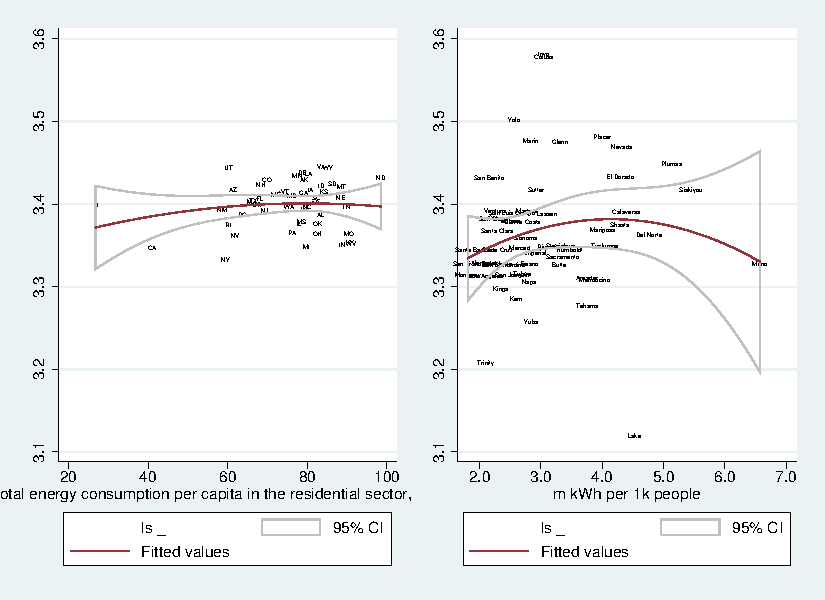
\includegraphics[width=6in]{graphsAndTables/stateCa.pdf}\centering
\caption{Happiness and total residential energy use across US states and
  residential electricity use across   
  California counties. Happiness is measured with ``In general, how satisfied are you with your life?'' on scale from 1=''very dissatisfied'' to 4=''very satisfied.''
We have also tried total energy consumption and its GDP
  intensity and relationship was also quite flat--see figure \ref{lfTETPBgdpLS}
  in supplementary material.}\label{stateCaPAP}
 \end{figure} % {\scriptsize Note: Country codes are in table \ref{ls} in
              % supplementary material. If country was observed in more than one
              % year, the data were averaged. }%PNAS readership should know US
              % state codes!

{\bf Over Time Movement.} It is well-known that happiness is related to income
in  a 
cross-section, but not over time \cite{easterlin74,easterlin12}. We
supplement our cross-sectional explorations with a look over time. We use General
Social Survey data.   %should be representatve %of regions but couldnt find any specific %evidence of that!
Happiness question reads "Taken all together, how would you say things are
      these days--would you say that you are very happy, pretty happy, or not
      too happy?" 1=''not to happy'', 2=''pretty happy'', 3=''very happy''. 
 Energy consumption is measured as total energy use per capita in
residential sector, the same measure as used for states in last section. 
Figure \ref{cenDivLsYrSm} shows happiness over time by
census division. There is not much co-movement. The two series correlate at only
.2. In short, neither in
cross-section, nor over time energy consumption is related to happiness in
the US. 

%TODO!!! add by hand happiness on yaxis(2) say in inkscape or sth
\begin{figure}[H]
 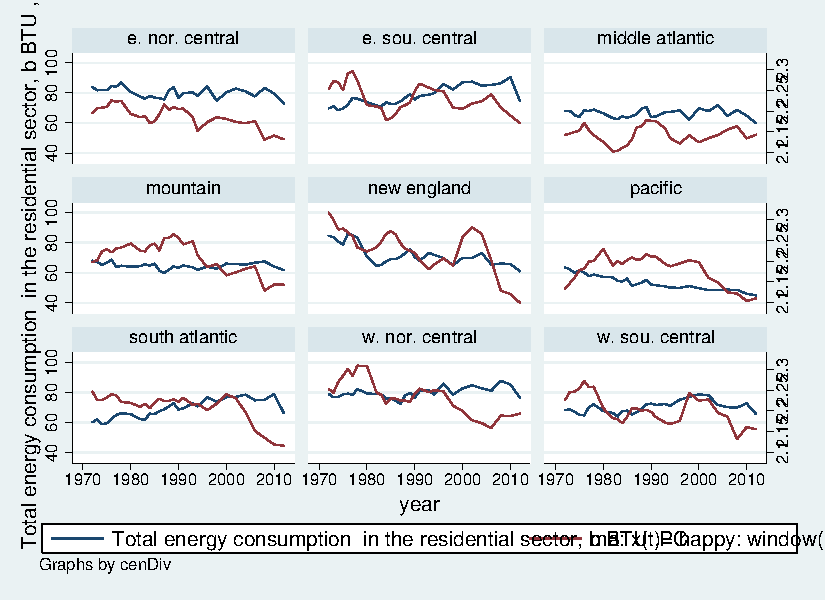
\includegraphics[width=5in]{graphsAndTables/cenDivLsYrSm.pdf}\centering
\caption{%TODO: 6-year moving average smoothened this shdl be on axis!!!
Happiness and total energy consumption
  in residential sector per capita. Correlation is .2 only (for
  unsmoothened series) 
 for unsmotthened happiness see fig \ref{cenDivLsYr} on
  p \pageref{cenDivLsYr}. Across countries there is not much variation in
  happiness over time, neither in energy use--see figure \ref{ebTS} in
  supplementary material. }\label{cenDivLsYrSm}
\end{figure}

Americans continue to consume large amounts of energy as compared to other
countries.  With a notable exception of California, energy use is
not decreasing, and in some cases energy use has increased. 
Also, Americans do not spend any less  on energy either--5-10\% of personal
expenditure is spent on energy over past 50 years, and if anything this amount
has  increased slightly  over the last decade \cite{bea-2-8-5}.
%   \url{http://burnanenergyjournal.com/what-goes-down-steins-law-and-the-cost-of-energy/}
% or \url{http://environmentalresearchweb.org/blog/energy-the-nexus-of-everything/}


\section*{\large \bf Discussion}

% Micah: We'll rewrite this later. The main goal is to (a) briefly summarize the most significant results; (b) outline the possible causal explanations and frameworks, and thus define the future research agenda; (c) describe potential interventions 

% 4/13
% TODO
% This jumps traight to causal conclusions.
% Need to be very careful about evaluating the evidence for the explanations we propose:
%   - energy efficiency 
%   - hedonic treadmill
% 	- conspicuous consumption (not the same as treadmill)
%	- positional good consumption
%	- risk-homeostasis based consumption (bigger cars)
%	- comparative national advantage in energy-intensive industries
%	- different baseline requirements for climate 
%
% For each of these explanations
%    - can we rule them out (or is their strong evidence against them) in the current data
%	 - what type of observation would be needed to test them (what level of aggregation of people, type of energy use, over time, an do we need natural expderiment)
%	 - what are appropriate interventions
%	 - which  of the interventions increase well being w/out increasing energy use, using current current feasible tech?
%	 - which of the interventions can increase well being w/out increasing energy use, requiring tech?

Happiness can be achieved at low levels of
energy consumption. At high level of energy consumption, such as
that in the  US, energy and happiness have a nil relationship. % If developed world changes from society of consumers
% to society of conservers, we will not suffer much in terms of
% happiness, if at all.
At the same time, however, it is widely assumed that the relationship is
positive. A useful concept of expected v experienced happiness helps to
illustrate it \cite{kahneman97ws} in figure \ref{fUT}. A decision on how much
energy we would like to  consume is based on expected happiness. But we are often (predictably) wrong.

\begin{figure}[H]
  \begin{centering}
    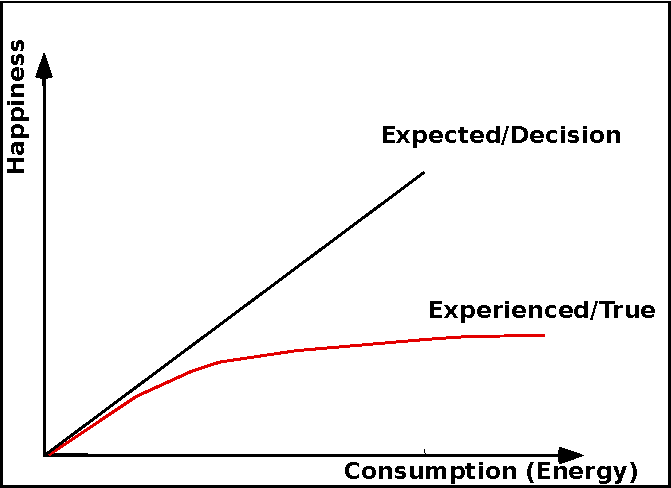
\includegraphics[height=2.7in]{graphsAndTables/utility}
    \caption{Expected vs. experienced utility or happiness. We make
      decision about income (or consumption) based on expected or
      decision happiness, but the experienced or true happiness is
      lower when we achieve greater  income or consumption.}\label{fUT}
  \end{centering}
\end{figure}


While in poorest countries, more  income and perhaps more energy
 is needed in some cases to increase happiness; in developed world, we arguably could  decrease
energy consumption without much loss in happiness. % can alse give some numbers on how much energy uses an american v
            % chinese etc
Perhaps, Indians and Chinese need to consume more energy, but not Americans. 
Texans could consume as much as Californians (they consume more than twice as
much) and no tragedy would happen. %http://www.eia.gov/state/rankings/
% Furthermore, it is unfair for the developed World to lecture developing
% countries about energy conservation without first making very substantial cuts
% at home.

There are a number of possible causal explanations. One possible cause that
happiness is higher for countries with lower energy intensity of GDP is the use
of more energy-efficient technologies--these technologies reduce energy inputs
for the same output of goods. Importantly, consumption can remain high at low
levels of pollution if there is not much energy used per GDP. %can elaborate a
                                %bit if needed
%better efficiency--less pollution per
%consumption--more good stuff without the bad stuff

Why energy use is not associated with happiness in the US? 
Consumption beyond a point does not buy happiness. Such consumption buys
position, but because everybody tries to oucompete everyone else, this race
cannot be won. A related cause is a ``hedonic treadmill'' \cite{brickman78cj}--increased consumption does not necessarily increase well-being due to hedonic-adaptation. In other words, more stuff
doesn't make people happy if basic needs are already satsified--hence positive
relationship between happiness and energy across countries, but no relationship
in the US. % --poor countries need to consume more enrgy in order to increase their
% happiness, but not the rich countries
 A related explanation can be made using Veblen's concept of conspicuous or
 wasteful consumption \cite{veblen05a, veblen05b}. Such consumption does not
 satisfy needs but simply aims to demostrate that
one is better than others. Much of such consumption wastes energy without gain
in wellbeing.% , for
% instance, mansions and large cars.  Many other examples are not necessarily conspicuous, 
% but they waste energy and have no clear contribution to lasting happiness, for
% instance, much of landscaping including unnatural ponds, fountains, and other items that
% define American suburbia.
Earlier, many social scientists suggested  that conspicuous consumption
does not make us any happier  \cite{csikszentmihalyi99, frank04, frank05, frank12}, but few actually test it. We contribute with a quantitative study of
the relationship between energy consumption and happiness. % and again, the only  study testing the
% effect of energy use on happiness was \cite{graef81}.
 Results suggests that  energy consumption can be substantially reduced
without making people less happy.  Now we turn to  possible interventions that could reduce energy consumption
 relatively painlessly. 

%NOT SURE IF WE NEED THIS
%  Similarly, increased income at country level does not lead over time to increased happiness--the so called Easterlin paradox
% \cite{easterlin74,easterlin10B}.  It is possible that some countries are more efficient because they have avoided this treadmill effect.
% Neither do conspicous consumption nor positional consumption result in
% happiness. There is more happiness gained from buying experience than buying
% things. For instanace, bowling, yoga, gardening result in more happiness than
% extra bedroom or larger house.  For most people,
% house is the biggest purchase they ever make and Americans tend to
% prefer big houses, but to afford them they need to commute longer
% distance. Humans adapt to big houses, but not to commute \cite{stutzer03,kahneman04,frank05}. 
%  Notably, both large houses and commute use energy that does not translate to happiness.  
%  Any luxury consumption (not only large houses) % SUVs, LV handbags
%  is not likely to result in lasting happiness because luxuries  are positional goods--people buy them to have a better position in a
% society, or to show that they are better than others--not to have a better quality of life.  The problem with
% positional goods is that acquiring them leads to consumption
% arms-race. You cannot win--you are  on hedonic treadmill.
% --we compare to others and, we
% adjust \citep{michalos85}
%  Due to this arms-race we ended up with
% ridiculously  big and expensive McMansions, SUVs, and other building
% blocks of American suburbia.

% What is the mechanism? Why energy consumption is not likely to buy much
% happiness?  There are several psychological explanations about causal pathways.
% We should buy experience, not things. Experience consumption results in more
% happiness than consumption of things. 
% That is  probably why  energy
% consumption in transportation brings most happiness out of different types of
% energy consumption, because much of
% transportation is about experience, for instance, travel, vacations. 
% % TODO from ls\_car lsPol and: 
% % Here psychological literature helps.
% Simply material consumption (where arguably most of the  the energy consumption
% falls) does not result in lasting happiness as opposed to experience
% consumption. Indeed, sustainable consumption does not necessarily mean less
% happiness, and there are many examples of activities low in carbon footprint but
% high in happiness such as gardening or yoga \cite{madjar06}. There is also
% consumption arms race that increases consumption, but not happiness. People are trying to outcompete each other in
% consumption but such race cannot be won and accordingly it does not result in lasting
% happpiness \cite{frank12}.% MAYBE hedonic adaptation etc etc
% % Finally,  pollution--energy cnsumption and $CO_2$ emissions correlate at above
% % .9, and pollution reduces happiness. %TODO cite


%------HOUSING guess irrelevant----------------------------
% One implication of the study is for housing: house is most expensive consumption
% item most people buy. Furthermore it costs considerable energy to build and
% maintain. The median house size in 1973 was 1,525 sq ft, and 2,169  sq ft in 2010.\footnote{\url{http://www.census.gov/const/C25Ann/sftotalmedavgsqft.pdf}}
% Surely, the families must have gotten bigger over that time. Well,
% actually they gotten smaller--in 1973 the average household size was
% 3.01, which dropped to 2.61 in
% 2010.\footnote{\url{http://www.census.gov/population/socdemo/hh-fam/tabHH-6.pdf};\url{http://quickfacts.census.gov/qfd/states/00000.html}}
% The problem with big houses is that it is never big enough anyway--we
% compare it to other houses, and size is an obvious metric. But others
% do the same and they get ever bigger houses all the time so we all end
% up with bigger houses but nobody is happier \cite{frank12}. ``A house may be large or small; as long as the neighboring houses are
% likewise small, it satisfies all social requirements for a
% residence. But let there arise next to the little house a palace, and
% the little house shrinks to a hut'' (Marx and Engels 1849, quoted in
% \cite{dittmann10}). \cite{dittmann10} find support for the above
% statement. \cite{luttmer05} also finds that the richer the neighbors,
% the less happy the person.
% \cite{firebaugh09} refine this relationship by confirming that people
% are happier in poor counties, but in  rich neighborhoods. 
%========================================================================

Two interventions to decrease energy consumption are suggested. First, we simply
need to increase awarness of what we have just described--that increasing
already substantial consumption does not buy much happiness, if any. Just as increasing increasing income
 beyond a point does not result in much happiness \cite{kahneman10}, increasing energy consumption beyond a point is not resulting in much happiness
 either as already suggested earlier \cite{mazur74, mazur11}. In short, happiness can be achieved at low
 levels of energy consumption--human flourishing requires energy to satisfy
 basic needs only. Second, we recommend higher taxes on non-renewable energy. 

It is striking that there were only three  attempts to
relate energy consumption to happiness.   % in 70s proxied 
 In a small sample of 55 countries, one early study used a set of 27 indicators to measure
 quality of life \cite{mazur74}, which was later extended over time \cite{mazur11}.
 A third study is a recent master
 thesis that  analyzes cross national data \cite{winfrey13}. But neither
 study  explores energy intensity of GDP, nor variation at finer geographic representation than a country.
 % We know that pollution makes
% us unhappy \cite{mackerron09,gandelman12,ferreira13}.
Furthermore, we contribute with a finding that energy consumption does contribute to happiness, if pollution is
taken into account. Results are in the supplementary material. This is a clear argument in favor of clean energy--if we can
consume energy without pollution, it should result in greater happiness. Until
we can to do so for vast majority of our energy needs, we should curb the energy consumption and
our wants or desires.

There is a need for future research in this important area. There have been many
calls to systmatically collect happiness data, and we should colect energy use data for the same persons. Suuch data would allow
to explore the relationship better at person level. There are many surveys
asking happiness question, for instance, World Values Surveys, General Social
Surveys and Eurobarometers, but they do not survey energy use. 

% Then there are needs v wants--how much energy we really need v what we want
% (which is endless). For instance, we need temperature in a dwelling to be above
% a freezing point, but we want temperature to be in 80s in winter, while 60s
% would be fine. We need some transportation--train or perhaps some car, but we
% want an SUV, and so forth. The point is that in the US, easily half of energy
% consumption is a want (for instance Texans consume twice as much as New
% Jersians--they would be fine if they consume at levels of New Jersey).% stover14

%  And equity and environmental justice--it is wildly
% recognized that there is income inequality \cite{piketty14} but there is
%  also plenty of environmental injustice--for instance Americans consume much
%  more resources than Indians, and of course within the US, recource consumption
%  varies enormously as well--for insance Texas consumes twice as much energy per
%  capita than New Jersey TODOciteFromOtehrMaterialHere. It is plainly no fair to
%  require poor countries such as India, or poor areas within countries or poor
%  people to care as much about conservation as the rich.
%  Furthermore, inequality in energy
%  consumption is in some ways more important than inequality in income, because
%  income is unlimited, while energy is (still most of energy comes from fossil
%  fuels TODOdbleCheck).  % stover14

% Energy efficiency is not ultimate solution and actually often backfires--it is
% like building more reoads or more lanes for traffic or loosening your belt for
% big belly--traffic increases, belly grows further and energy consumption grows
% furtehr too!
% %http://www.nytimes.com/2014/10/09/opinion/the-problem-with-energy-efficiency.html?hp&action=click&pgtype=Homepage&module=c-column-top-span-region&region=c-column-top-span-region&WT.nav=c-column-top-span-region&_r=0
% %hwys and loosening belt come from duany book

% Energy use and environmental iussies are  increasingy political in the US, and
% may even become a key issue in the near furtre. There is now a surfge in
% political advertising \cite{davenport_nyt_oct21_14}.


\section*{\large \bf Materials and Methods}
%boilerplate following
% http://www.pnas.org/content/109/49/19949.full.pdf  
% http://www.pnas.org/content/112/3/725.full.pdf
% http://www.pnas.org/content/109/25/9775.full.pdf
All happiness measures come from surveys representative of given areas. Such measures are reasonably valid and
reliable \cite{diener13b}. % , consistent and stable? or means same as valid, reliable?
One caveat is cross-cultural comparability \cite{diener03b}. The cross
country results that we report, however, show  strong relationship and it is very
unlikely that all that is due to measurement. Furthermore, we mostly use data
within the US. % LATER Energy measures  discuss their reliability, validity etc just google around.
We focus on simple relationships. Multivariate regressions are
discussed in the supplementary online material. 


\noindent\textbf{ACKNOWLEDGMENTS.} We thank... 


\newpage
%\bibliography{/home/aok/papers/root/tex/ebib.bib}
\begin{thebibliography}{10}

\bibitem{mackay08}
MacKay D (2008) {\em Sustainable Energy-without the hot air}.
\newblock (UIT Cambridge).

\bibitem{arrow04}
Arrow K et~al. (2004) Are we consuming too much?
\newblock {\em Journal of Economic Perspectives} pp. 147--172.

\bibitem{soytas07}
Soytas U, Sari R, Ewing BT (2007) Energy consumption, income, and carbon
  emissions in the united states.
\newblock {\em Ecological Economics} 62(3):482--489.

\bibitem{stiglitz09al}
Stiglitz J, Sen A, Fitoussi J (2009) Report by the commission on the
  measurement of economic performance and social progress.
\newblock {\em Available at www.stiglitz-sen-fitoussi.fr}.

\bibitem{kenny_businessweek_aug_29_14}
Kenny C (2014) Poor countries shouldn't sacrifice growth to fight climate
  change.
\newblock {\em Businessweek} (August).

\bibitem{gordon_wsj_may_29_14}
Gordon K (2014) Cutting energy without self sacrifice.
\newblock {\em Wall Street Journal} (May).

\bibitem{carter_pbs_apr_18_77}
Carter J (1977) Proposed energy policy.
\newblock {\em Public Broadcasting Service} (May).

\bibitem{smil05}
Smil V (2005) Creating the twentieth century: technical innovations of
  1867-1914 and their lasting impact.
\newblock {\em OUP Catalogue}.

\bibitem{mackerron09}
MacKerron G, Mourato S (2009) Life satisfaction and air quality in london.
\newblock {\em Ecological Economics} 68(5):1441--1453.

\bibitem{gandelman12}
Gandelman N, Piani G, Ferre Z (2012) Neighborhood determinants of quality of
  life.
\newblock {\em Journal of Happiness Studies} 13:547--563.

\bibitem{ferreira13}
Ferreira S et~al. (2013) Life satisfaction and air quality in europe.
\newblock {\em Ecological Economics} 88:1--10.

\bibitem{kallis11}
Kallis G (2011) In defence of degrowth.
\newblock {\em Ecological Economics} 70(5):873--880.

\bibitem{kallis12}
Kallis G, Kerschner C, Martinez-Alier J (2012) The economics of degrowth.
\newblock {\em Ecological Economics} 84:172--180.

\bibitem{pretty13}
Pretty J (2013) The consumption of a finite planet: well-being, convergence,
  divergence and the nascent green economy.
\newblock {\em Environmental and Resource Economics} 55(4):475--499.

\bibitem{mazur11}
Mazur A (2011) Does increasing energy or electricity consumption improve
  quality of life in industrial nations?
\newblock {\em Energy Policy} 39(5):2568--2572.

\bibitem{brickman78cj}
Brickman P, Coates D, Janoff-Buman R (1978) Lottery winners and accident
  victims: Is happiness relative?
\newblock {\em Journal of Personality and Social Psychology} 36:917--927.

\bibitem{easterlin74}
Easterlin RA (1974) {\em Does Economic Growth Improve the Human Lot?} eds.{}
  David PA, Reder MW.
\newblock (New York: Academic Press, Inc.), Vol.{}~89, pp. 98--125.

\bibitem{easterlin10B}
Easterlin RA, McVey LA, Switek M, Sawangfa O, Zweig JS (2010) The
  happiness--income paradox revisited.
\newblock {\em Proceedings of the National Academy of Sciences}
  107(52):22463--22468.

\bibitem{mazur74}
Mazur A, Rosa E (1974) Energy and life-style.
\newblock {\em Science (New York, NY)} 186(4164):607.

\bibitem{easterlin12}
Easterlin RA, Morgan R, Switek M, Wang F (2012) China's life satisfaction,
  1990--2010.
\newblock {\em Proceedings of the National Academy of Sciences}
  109(25):9775--9780.

\bibitem{bea-2-8-5}
BEA (2014) Table 2.8.5. personal consumption expenditures by major type of
  product, monthly.
\newblock {\em Bureau of Economic Analysis}.

\bibitem{veblen05a}
Veblen T (2005) {\em Conspicuous consumption}.
\newblock (ePenguin) Vol.{}~38.

\bibitem{veblen05b}
Veblen T (2005) {\em The theory of the leisure class; an economic study of
  institutions}.
\newblock (Aakar Books).

\bibitem{csikszentmihalyi99}
Csikszentmihalyi M (1999) If we are so rich, why aren't we happy?
\newblock {\em American psychologist} 54(10):821.

\bibitem{frank04}
Frank RH (2004) How not to buy happiness.
\newblock {\em Daedalus} 133(2):69--79.

\bibitem{frank05}
Frank RH (2005) {\em Does Absolute Income Matter} eds.{} Bruni L, Porta PL.
\newblock (Oxford University Press).

\bibitem{frank12}
Frank R (2012) {\em The Darwin economy: Liberty, competition, and the common
  good}.
\newblock (Princeton University Press).

\bibitem{madjar06}
Madjar M, Ozawa T (2006) Happiness and sustainable consumption: Psychological
  and physical rebound effects at work in a tool for sustainable design.
\newblock {\em The International Journal of Life Cycle Assessment}
  11(1):105--115.

\bibitem{kahneman10}
Kahneman D, Deaton A (2010) High income improves evaluation of life but not
  emotional well-being.
\newblock {\em Proceedings of the National Academy of Sciences}
  107(38):16489--16493.

\bibitem{winfrey13}
Winfrey EMV (2013) Ph.D. thesis (Georgetown University).

\bibitem{diener13b}
Diener E, Inglehart R, Tay L (2013) Theory and validity of life satisfaction
  scales.
\newblock {\em Social Indicators Research} 112(3):497--527.

\bibitem{diener03b}
Diener E, Suh EM, eds. (2003) {\em Culture and Subjective Well-Being}.
\newblock (MIT Press).

\bibitem{iea14}
Agency TIE (2007) Energy use in the new millennium.
\newblock {\em Energy Indicators}.

\bibitem{graef81}
Graef R, McManama~Gianinno S, Csikszentmihalyi M (1981) {\em Energy consumption
  in leisure and perceived happiness} ed.{} Claxton JM.
\newblock (New York: Praeger), pp.~--.

\bibitem{csikszentmihalyi14}
Csikszentmihalyi M, Graef R, Gianinno SM (2014) in {\em Flow and the
  Foundations of Positive Psychology}.
\newblock (Springer), pp. 127--133.

\bibitem{dietz09}
Dietz T, Rosa EA, York R (2009) Environmentally efficient well-being:
  Rethinking sustainability as the relationship between human well-being and
  environmental impacts.
\newblock {\em Human Ecology Review} 16(1):114--123.

\bibitem{jorgenson14B}
Jorgenson AK, Alekseyko A, Giedraitis V (2014) Energy consumption, human
  well-being and economic development in central and eastern european nations:
  A cautionary tale of sustainability.
\newblock {\em Energy Policy} 66:419--427.

\bibitem{steinberger10}
Steinberger JK, Roberts JT (2010) From constraint to sufficiency: The
  decoupling of energy and carbon from human needs, 1975--2005.
\newblock {\em Ecological Economics} 70(2):425--433.

\bibitem{dias06}
Dias RA, Mattos CR, P~Balestieri JA (2006) The limits of human development and
  the use of energy and natural resources.
\newblock {\em Energy Policy} 34(9):1026--1031.

\bibitem{klugman11}
Klugman J, Rodr{\'\i}guez F, Choi HJ (2011) The hdi 2010: new controversies,
  old critiques.
\newblock {\em The Journal of Economic Inequality} 9(2):249--288.

\bibitem{veenhoven96B}
Veenhoven R (1996) Happy life-expectancy.
\newblock {\em Social Indicators Research} 39(1):1--58.

\bibitem{weinhold12}
Weinhold D (2012) The happiness-reducing costs of noise pollution.
\newblock {\em Journal of regional science}.

\bibitem{welsch05}
Welsch H (2005) Environment and happiness: Valuation of air pollution using
  life satisfaction data.
\newblock {\em Ecological Economics} 58:801--813.

\bibitem{ericson14}
Ericson T, Kj{\o}nstad BG, Barstad A (2014) Mindfulness and sustainability.
\newblock {\em Ecological Economics} 104:73--79.

\bibitem{brown05}
Brown KW, Kasser T (2005) Are psychological and ecological well-being
  compatible? the role of values, mindfulness, and lifestyle.
\newblock {\em Social Indicators Research} 74(2):349--368.

\bibitem{corral11}
Corral-Verdugo V, Mireles-Acosta J, Tapia-Fonllem C, Fraijo-Sing B (2011)
  Happiness as correlate of sustainable behavior: A study of pro-ecological,
  frugal, equitable and altruistic actions that promote subjective wellbeing.
\newblock {\em Human Ecology Review} 18(2):95--104.

\bibitem{durkheim50}
Durkheim E ([1895] 1950) {\em The Rules of Sociological Method}.
\newblock (New York: The Free Press).

\bibitem{steel08}
Steel P, Schmidt J, Shultz J (2008) Refining the relationship between
  personality and subjective well-being.
\newblock {\em Psychological bulletin} 134(1):138--161.

\bibitem{veenhoven08}
Veenhoven R (2008) {\em Sociological theories of subjective well-being} eds.{}
  Eid M, Larsen R.
\newblock (The Guilford Press, New York), pp. 44--61.

\bibitem{diener09}
Diener E (2009) {\em Well-being for public policy}.
\newblock (Oxford University Press).

\bibitem{michalos85}
Michalos A (1985) Multiple discrepancies theory (mdt).
\newblock {\em Social Indicators Research} 16(4):347--413.

\bibitem{veenhoven95}
Veenhoven R, Ehrhardt J (1995) The cross-national pattern of happiness: Test of
  predictions implied in three theories of happiness.
\newblock {\em Social Indicators Research} 34(1):33--68.

\bibitem{veenhoven14b}
Veenhoven R (2014) Livability theory.
\newblock {\em Encyclopedia of Quality of Life and Well-Being Research} pp.
  3645--3647.

\bibitem{marshallCL14}
Marshall A (2014) How skyrocketing development in texas could suck the state
  dry.
\newblock {\em City Lab}.

\bibitem{abdallah08al}
Abdallah S, Thompson S, Marks N (2008) Estimating worldwide life satisfaction.
\newblock {\em Ecological Economics} 65(1):35--47.

\bibitem{brereton08}
Brereton F, Clinch J, Ferreira S (2008) Happiness, geography and the
  environment.
\newblock {\em Ecological Economics} 65(2):386--396.

\bibitem{fuguitt90}
Fuguitt GV, Brown DL (1990) Residential preferences and population
  redistribution: 72-1988.
\newblock {\em Demography} 27(4):589--600.

\bibitem{fuguitt75}
Fuguitt GV, Zuiches JJ (1975) Residential preferences and population
  distribution.
\newblock {\em Demography} 12(3):491--504.

\bibitem{aok_hea_spr}
Okulicz-Kozaryn A (2014) Natural sprawl.
\newblock {\em Forthcoming in Administration \& Society (Disputatio Sine Fine
  section)}.

\bibitem{aok11a}
Berry BJ, Okulicz-Kozaryn A (2011) An urban-rural happiness gradient.
\newblock {\em Urban Geography} 32(6):871--883.

\end{thebibliography}




\newpage
\section{\huge ONLINE SUPPLEMENATRY MATERIAL}

\tableofcontents

\section{Country-level additional information}
%TODO adjust thi sstuff to now using WDH instead ofg WVS!!

Table
\ref{var_des} lists variables used and their definitions for cross-country
analysis. 

\begin{table}[H]\centering\footnotesize
 \caption{\label{var_des} Variable definitions}
\begin{tabular} {p{1.5in}p{4.5in}}   \hline
name & description   \\ \hline
  happiness & "All things considered, how satisfied are you with your life as a whole these days?" 1="dissatisfied" to 10="satisfied"; WVS \\
  PCGDP & GDP per capita (constant 2005 US\$); Code: NY.GDP.PCAP.KD; "GDP per capita is gross domestic product divided by midyear population. GDP is the sum of gross value added by all resident producers in the economy plus any product taxes and minus any subsidies not included in the value of the products. It is calculated without making deductions for depreciation of fabricated assets or for depletion and degradation of natural resources. Data are in constant 2005 U.S. dollars."; WB \\
  energy use, pc & Energy use (kg of oil equivalent per capita); Code: EG.USE.PCAP.KG.OE "Energy use refers to use of primary energy before transformation to other end-use fuels, which is equal to indigenous production plus imports and stock changes, minus exports and fuels supplied to ships and aircraft engaged in international transport."; WB \\
  unemployment, \% & Unemployment, total (\% of total labor force) (modeled ILO estimate); Code: SL.UEM.TOTL.ZS; "Unemployment refers to the share of the labor force that is without work but available for and seeking employment."; WB \\
  co2 emissions, pc & CO2 emissions (metric tons per capita); Code: EN.ATM.CO2E.PC; "Carbon dioxide emissions are those stemming from the burning of fossil fuels and the manufacture of cement. They include carbon dioxide produced during consumption of solid, liquid, and gas fuels and gas flaring."; WB \\
  female life expectancy & Life expectancy at birth, female (years); Code: SP.DYN.LE00.FE.IN; "Life expectancy at birth indicates the number of years a newborn infant would live if prevailing patterns of mortality at the time of its birth were to stay the same throughout its life." WB\\
  road sector gasoline fuel consumption, pc & Road sector gasoline fuel consumption per capita (kg of oil equivalent); Code: IS.ROD.SGAS.PC; "Gasoline is light hydrocarbon oil use in internal combustion engine such as motor vehicles, excluding aircraft."; WB \\
  percent urban & population (\% of total); Code: SP.URB.TOTL.IN.ZS; "Urban population refers to people living in urban areas as defined by national statistical offices. It is calculated using World Bank population estimates and urban ratios from the United Nations World Urbanization Prospects." WB\\
  maximum temperature in January & "near-surface temperature maximum (degrees Celsius)" ; TYN\_CY \\
  maximum temperature in July & "near-surface temperature maximum (degrees Celsius)" ; TYN\_CY \\
\hline\end{tabular}\end{table}


{\scriptsize \noindent Variable sources. WVS: World Values Survey \url{www.worldvaluessurvey.org};
TYN\_CY: Tyndall Centre (\url{www.tyndall.ac.uk}) Mitchell,T.D., Hulme,M., and
New,M., 2002: Climate data for political areas. Area
34:109-112. \url{http://www.cru.uea.ac.uk/~timm/cty/obs/TYN_CY_1_1_var-table.html};
WB: World Bank \url{http://data.worldbank.org}}

 \begin{scriptsize}  \begin{center} \begin{longtable}{llllllllllllll} \caption{
Key
variables
for
each
country.}
\label{ls}
\\
\hline
\multicolumn{1}{p{.75in}}{Country
Code
(ISO
2
digits)}
&
\multicolumn{1}{p{.75in}}{Country
Name}
&
\multicolumn{1}{p{.75in}}{happiness
(WDH)}&
\multicolumn{1}{p{.75in}}{energy
use,
pc}&
\multicolumn{1}{p{.75in}}{PCGDP}&
\multicolumn{1}{p{.75in}}{co2
emissions,
pc}&
\multicolumn{1}{p{.75in}}{female
life
expectancy}
&
\multicolumn{1}{p{.75in}}{}
\\
\hline
\endfirsthead
\multicolumn{3}{p{.75in}}
{{\bfseries
\tablename\
\thetable{}
--
continued
from
previous
page}}
\\
\hline
\multicolumn{1}{p{.75in}}{Country
Code
(ISO
2
digits)}
&
\multicolumn{1}{p{.75in}}{Country
Name}
&
\multicolumn{1}{p{.75in}}{happiness
(WDH)}&
\multicolumn{1}{p{.75in}}{energy
use,
pc}&
\multicolumn{1}{p{.75in}}{PCGDP}
&
\multicolumn{1}{p{.75in}}{co2
emissions,
pc}&
\multicolumn{1}{p{.75in}}{female
life
expectancy}
&
\multicolumn{1}{p{.75in}}{}\\
\hline
\endhead
\hline
\multicolumn{5}{r}{{Continued
on
next
page}}
\\
\endfoot
\hline
\endlastfoot

AD&Andorra&6.8&&31,107&7.1&\\
AE&United Arab Emirates&7.3&10,447&40,623&28.0&76\\
AF&Afghanistan&4.1&&267&0.1&58\\
AL&Albania&4.6&671&2,773&1.3&79\\
AM&Armenia&5.0&780&1,551&1.4&76\\
AO&Angola&4.3&589&1,798&1.1&49\\
AR&Argentina&7.3&1,733&5,349&4.1&78\\
AT&Austria&7.4&3,911&37,097&8.4&82\\
AU&Australia&7.7&5,605&33,593&17.6&83\\
AZ&Azerbaijan&5.3&1,467&1,740&4.2&72\\
BA&Bosnia and Herzegovina&5.8&1,289&2,791&6.6&78\\
BD&Bangladesh&5.3&166&421&0.3&68\\
BE&Belgium&7.3&5,544&35,692&10.4&82\\
BF&Burkina Faso&4.4&&395&0.1&53\\
BG&Bulgaria&4.4&2,490&3,651&6.1&76\\
BI&Burundi&2.9&&148&0.0&51\\
BJ&Benin&3.0&327&536&0.4&58\\
BO&Bolivia&6.3&499&1,029&1.3&67\\
BR&Brazil&7.5&1,160&4,771&1.9&75\\
BW&Botswana&4.7&1,046&5,347&2.4&48\\
BY&Belarus&5.2&2,740&3,077&5.9&75\\
BZ&Belize&6.6&604&3,977&1.7&75\\
CA&Canada&7.8&8,106&35,353&16.9&83\\
CD&Congo, Dem. Rep.&4.4&368&220&0.0&49\\
CF&Central African Republic&4.6&&360&0.1&47\\
CG&Congo, Rep.&3.7&302&1,685&0.3&55\\
CH&Switzerland&8.0&3,528&52,041&5.5&84\\
CI&Cote d'Ivoire&4.4&490&956&0.4&48\\
CL&Chile&6.7&1,703&7,452&3.8&81\\
CM&Cameroon&3.9&371&909&0.2&53\\
CN&China&6.3&1,292&1,752&4.1&75\\
CO&Colombia&7.7&634&3,410&1.4&76\\
CR&Costa Rica&8.5&877&4,651&1.6&81\\
CY&Cyprus&7.1&2,249&22,498&7.4&81\\
CZ&Czech Republic&6.5&4,279&12,458&11.8&79\\
DE&Germany&7.1&4,075&34,054&9.8&82\\
DJ&Djibouti&5.7&178&924&0.6&60\\
DK&Denmark&8.3&3,558&46,939&9.1&80\\
DO&Dominican Republic&7.5&771&3,754&2.2&75\\
DZ&Algeria&5.4&961&2,884&3.0&71\\
EC&Ecuador&6.4&742&2,932&2.0&77\\
EE&Estonia&6.0&3,737&9,666&12.1&78\\
EG&Egypt, Arab Rep.&5.7&808&1,278&2.3&72\\
ES&Spain&7.2&3,100&25,523&7.5&84\\
ET&Ethiopia&4.2&382&163&0.1&57\\
FI&Finland&7.9&6,691&36,747&11.4&82\\
FR&France&6.6&4,181&33,576&6.0&84\\
GB&United Kingdom&7.2&3,591&37,282&8.8&81\\
GE&Georgia&4.3&658&1,432&1.1&76\\
GH&Ghana&5.2&403&503&0.4&59\\
GN&Guinea&4.5&&303&0.1&53\\
GR&Greece&6.4&2,645&21,170&8.7&82\\
GT&Guatemala&7.2&625&2,176&0.9&73\\
GY&Guyana&6.5&646&1,097&2.0&68\\
HK&Hong Kong SAR, China&6.6&2,003&25,951&5.7&85\\
HN&Honduras&7.0&566&1,383&1.0&74\\
HR&Croatia&6.0&1,952&9,815&5.1&79\\
HT&Haiti&3.9&264&466&0.2&61\\
HU&Hungary&5.5&2,587&10,409&5.6&77\\
ID&Indonesia&6.3&785&1,268&1.5&71\\
IE&Ireland&7.6&3,484&46,692&10.4&81\\
IL&Israel&7.0&2,894&19,659&9.5&82\\
IN&India&5.5&486&735&1.3&65\\
IQ&Iraq&4.7&999&1,874&3.4&73\\
IR&Iran, Islamic Rep.&5.9&2,359&2,690&6.7&73\\
IS&Iceland&8.2&13,136&52,394&7.3&83\\
IT&Italy&6.7&3,049&30,633&7.9&84\\
JM&Jamaica&6.7&1,439&4,190&4.1&74\\
JO&Jordan&5.9&1,140&2,315&3.5&74\\
JP&Japan&6.5&3,992&35,282&9.5&86\\
KE&Kenya&3.7&451&525&0.3&56\\
KG&Kyrgyz Republic&5.5&487&484&1.0&72\\
KH&Cambodia&4.9&281&457&0.2&69\\
KR&Korea, Rep.&6.0&4,343&18,350&9.9&82\\
KW&Kuwait&6.6&10,513&32,141&29.0&75\\
KZ&Kazakhstan&6.1&3,371&3,595&11.7&72\\
LA&Lao PDR&6.2&&471&0.2&65\\
LB&Lebanon&4.7&1,366&5,590&4.4&79\\
LK&Sri Lanka&5.1&447&1,245&0.6&77\\
LR&Liberia&4.3&&191&0.2&56\\
LT&Lithuania&5.5&2,649&7,487&4.1&78\\
LU&Luxembourg&7.7&8,552&79,226&22.1&82\\
LV&Latvia&5.4&1,947&6,746&3.2&77\\
MA&Morocco&5.4&422&1,947&1.4&71\\
MD&Moldova&4.9&905&786&1.2&72\\
ME&Montenegro&5.2&1,736&3,781&3.6&77\\
MG&Madagascar&3.7&&280&0.1&62\\
MK&Macedonia, FYR&4.7&1,340&2,890&5.5&76\\
ML&Mali&4.7&&443&0.0&51\\
MN&Mongolia&5.7&1,092&987&3.5&69\\
MR&Mauritania&4.9&&705&0.5&62\\
MT&Malta&7.1&2,010&15,024&6.2&82\\
MW&Malawi&6.2&&219&0.1&49\\
MX&Mexico&7.9&1,480&7,809&3.8&78\\
MY&Malaysia&6.5&2,334&5,457&6.6&76\\
MZ&Mozambique&3.8&404&303&0.1&49\\
NA&Namibia&5.2&604&3,506&1.1&59\\
NE&Niger&3.8&&263&0.1&54\\
NG&Nigeria&5.7&742&749&0.7&49\\
NI&Nicaragua&7.1&509&1,147&0.8&75\\
NL&Netherlands&7.6&4,760&39,400&10.5&82\\
NO&Norway&7.9&5,880&64,397&9.3&82\\
NP&Nepal&5.3&358&322&0.1&65\\
NZ&New Zealand&7.5&4,191&26,786&8.2&82\\
PA&Panama&7.8&859&4,727&2.0&79\\
PE&Peru&6.2&485&2,713&1.3&75\\
PH&Philippines&5.9&459&1,190&0.9&71\\
PK&Pakistan&5.0&472&672&0.8&66\\
PL&Poland&6.4&2,432&8,036&8.0&79\\
PS&West Bank and Gaza&4.9&&1,247&0.5&73\\
PT&Portugal&5.7&2,400&18,307&5.9&81\\
PY&Paraguay&6.8&696&1,504&0.7&73\\
QA&Qatar&6.8&19,868&54,880&54.2&78\\
RO&Romania&5.7&1,791&4,607&4.4&76\\
RS&Serbia&5.4&2,166&3,261&6.9&76\\
RU&Russian Federation&5.5&4,516&5,210&11.2&73\\
RW&Rwanda&4.3&&271&0.1&56\\
SA&Saudi Arabia&6.5&5,692&13,381&15.5&76\\
SD&Sudan&5.0&384&675&0.3&62\\
SE&Sweden&7.8&5,532&40,050&5.6&83\\
SG&Singapore&6.9&5,454&28,541&7.7&82\\
SI&Slovenia&6.9&3,529&17,647&7.8&81\\
SK&Slovak Republic&5.9&3,393&11,443&7.1&78\\
SL&Sierra Leone&3.5&&315&0.1&42\\
SN&Senegal&4.5&249&752&0.5&62\\
SV&El Salvador&6.7&718&2,790&1.1&75\\
SY&Syrian Arab Republic&5.9&1,046&1,518&2.9&76\\
TD&Chad&5.4&&547&0.0&49\\
TG&Togo&2.6&427&389&0.2&55\\
TH&Thailand&6.6&1,437&2,621&3.7&76\\
TJ&Tajikistan&5.1&341&326&0.4&69\\
TM&Turkmenistan&7.2&3,911&1,769&9.5&69\\
TN&Tunisia&5.9&840&3,214&2.3&76\\
TR&Turkey&5.6&1,265&6,803&3.6&76\\
TT&Trinidad and Tobago&7.0&12,286&12,048&25.7&73\\
TZ&Tanzania&2.8&429&367&0.1&54\\
UA&Ukraine&5.0&2,866&1,734&6.8&74\\
UG&Uganda&4.8&&319&0.1&53\\
US&United States&7.4&7,725&43,146&19.3&80\\
UY&Uruguay&6.7&940&5,310&1.8&79\\
UZ&Uzbekistan&6.0&1,910&552&4.6&71\\
VE&Venezuela, RB&7.5&2,313&5,503&6.7&76\\
VN&Vietnam&6.1&485&685&1.1&79\\
YE&Yemen, Rep.&4.8&313&820&1.0&63\\
ZA&South Africa&5.8&2,658&5,149&8.7&55\\
ZM&Zambia&5.0&621&626&0.2&47\\
ZW&Zimbabwe&3.0&743&498&0.8&45\\
\end{longtable} \end{center} \end{scriptsize}   


\begin{figure}[H]
 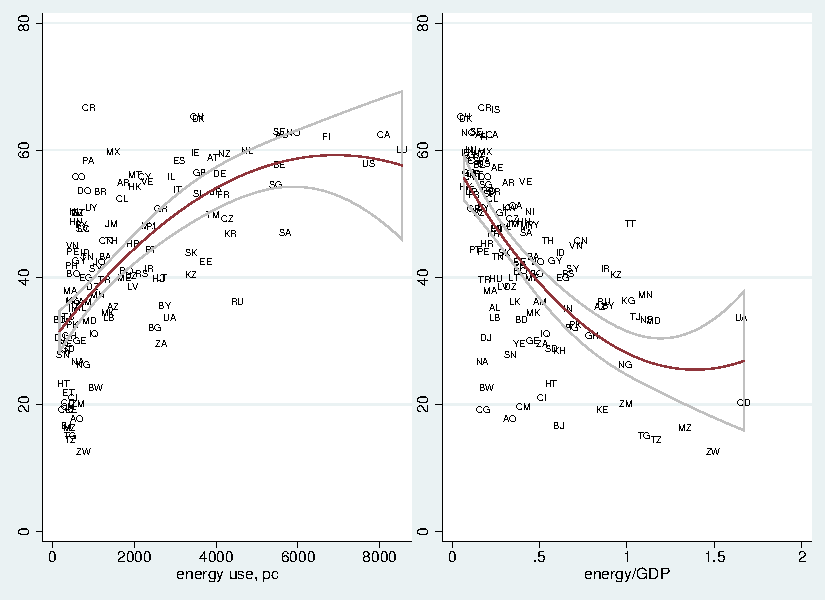
\includegraphics[width=6in]{graphsAndTables/couWdhEneGdpHly.pdf}\centering
\caption{Happy Life Years as a Dependent Variable}\label{hly}
\end{figure}


\subsection{regression framework: taking into account more factors} 

It is critical to control for percoent urban or population density, because
urban or dense areas are less happy and more energy efficient, and hence
omission of this variable leads to positive bias on energy use--the estimated
coefficient   is larger than it should be in a bivariate case. Indeed, bivariate
relationship appears positive. 

The bottom line is that there appears to be weak relationship betwen electricity
consumption and happiness, but it disappears or indeed becomes negative when
taking into account social support. One explanation is that people who consumer
more electricity, need to work more, and have less time for social stuff which
is iomportant for happiness. Per Bowling Alone, we do less and less social stuff
and robert frank--need to focus on non-pecuniary domain!

Regression results are set in table \ref{regA}. First we start with an ols
model. All ols regressions control for year dummies--again, different countries
were surveyed in different years. Energy consumption results in greater
happiness (ols1), but when controlling for PCGDP, the relationship disappears
(ols2). Addition of percent urban, unemployment rate and life expectancy (ols3)
makes the relationship actually significantly negative.  Addition of maximum
temperatures in January and July (ols4) makes it positive again but still
insignificant.  A very interesting thing occurs in column ols5--addition of
$CO_2$ makes energy positive and significant.\footnote{The two variables are
  correlated at .91. And $CO_2$ is negative as expected. Energy correlates at .38
  with happiness, and $CO_2$ correlates at .29 (positive, too).}
 Hence, energy consumption would increase happiness if not emissions. This may
 point to clean energy (wind, solar, etc) as a solution. 

Furthemore, in such a diverse sample of countries, there is some unobserved
heterogeneity. Two fixed effects model follow (temperature drops out, because we
 only have temperature for country for one time period). Yet comfortingly
 results are similar to ols, when not controling for $CO_2$, results ar weakly
 positive (fe1), but when adding $CO_2$ control results become significant
 (fe2). Again, we intrpret it  that energy consumption WITHOUT pollution would
 contribute more to happiness than just energy consumption.  

\begin{figure}[H]
 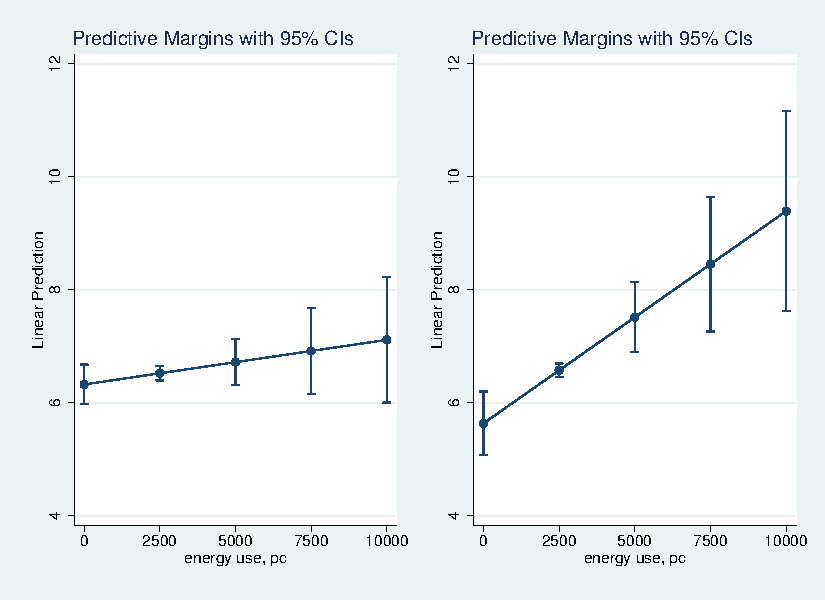
\includegraphics[width=6in]{graphsAndTables/ols4ols5.pdf}\centering
\caption{WVS all countries, first is ols4; second is ols5--the latter controls
  for co2--if we could have energy without pollution it would increase happiness! }\label{ols4ols5}
\end{figure}
{\scriptsize Note: Country codes are in table \ref{ls} in supplementary
  material. If country was observed in more than one year, the data were averaged.}


\begin{table}[H]\centering \caption{regA} \label{regA} \begin{scriptsize} \begin{tabular}{p{1.4in}p{.43in}p{.43in}p{.43in}p{.43in}p{.43in}p{.43in}p{.43in}p{.43in}p{.43in}p{.43 in}p{.43in}p{.43 in}}\hline                     &        ols1   &        ols2   &        ols3   &        ols4   &        ols5   &         fe1   &         fe2   \\
energy use, pc      &       0.000***&      -0.000+  &      -0.000*  &       0.000   &       0.000** &       0.001+  &       0.001*  \\
PCGDP               &               &       0.000***&       0.000***&       0.000** &       0.000*  &       0.000   &      -0.000   \\
percent urban       &               &               &       0.018** &      -0.001   &      -0.001   &       0.019   &       0.030   \\
unemployment, \%     &               &               &      -0.026*  &      -0.008   &      -0.002   &       0.010   &       0.009   \\
female life expectancy&               &               &       0.006   &       0.050** &       0.057***&      -0.002   &      -0.003   \\
maximum temperature in January&               &               &               &       0.045***&       0.049***&               &               \\
maximum temperature in July&               &               &               &      -0.019*  &      -0.014   &               &               \\
co2 emissions, pc   &               &               &               &               &      -0.108** &               &      -0.262   \\
constant            &       6.592***&       6.693***&       5.473***&       2.725*  &       1.921   &       3.657   &       3.245   \\
N                   &         163   &         162   &         139   &         139   &         139   &         139   &         139   \\
 \hline\multicolumn{6}{l}{+p$<$0.10 *p$<$0.05 **p$<$0.01 ***p$<$0.001; robust standard errors} \end{tabular}\end{scriptsize}\end{table}

\begin{verbatim}
             |   ene   gdp   urb   un   lexp  janMax julMax
-------------+---------------------------------------------------------------
         ene |   1.0 
         gdp |   0.7*  1.0 
         urb |   0.5*  0.5*  1.0 
          un |  -0.1* -0.2*  0.0   1.0 
        lexp |   0.5*  0.5*  0.7* -0.0   1.0 
      janMax |  -0.4* -0.3* -0.1  -0.0  -0.4*  1.0 
      julMax |  -0.3* -0.3* -0.3*  0.0  -0.2*  0.2*  1.0 
         co2 |   0.9*  0.6*  0.5* -0.0   0.4* -0.4* -0.2*

\end{verbatim}

\section{State-level additional results}
\subsection{How do we use energy in the US?}

Energy use is slightly increasing in the US
\url{http://www.eia.gov/todayinenergy/detail.cfm?id=4690}, and quite a bit in
the World. 
Energy use in the US is farily flat over past 40 yeaars at 70m btu
pc.\url{http://www.eia.gov/todayinenergy/detail.cfm?id=3590}, and coasts consume
less than inland middle
\url{http://energy.gov/maps/2009-energy-consumption-person?page=0%2C1}. 
Use by sector in the US: 22\% residential, 18\% commercial, 32\% industrial, and
28\% transportation.\url{http://www.eia.gov/consumption/}. 


For the US CBO produced a handy chart \url{http://www.cbo.gov/publication/43232} or \url{http://www.cbo.gov/sites/default/files/43232-infographic-EnergySecurity.pdf}

Some popular media description
\url{http://www.theatlantic.com/technology/archive/2013/08/a-very-short-history-of-how-americans-use-energy-at-home/278329/}

We know how energy is used in residential sector in the US ( we also know it for
other sectors but we do not focus on them)--all data are here
\url{http://www.eia.gov/forecasts/aeo/MT_residentialdemand.cfm}. FOr residential
sector
\url{http://www.eia.gov/oiaf/aeo/tablebrowser/aeo_query_server/?event=ehExcel.getFile&study=AEO2014&region=0-0&cases=ref2014-d102413a&table=4-AEO2014&yearFilter=0}:
table AEO2014: 


%LATER may see footnotes for this table
\begin{table}[H]\centering\footnotesize
\caption{\label{freq_im_god} Total Energy Consumption by End Use; quadrillion
  Btu, 2011}
\begin{tabular}{lll}   \hline 
Space Heating&	5.6\\
Space Cooling&	2.6\\
Water Heating&	2.7\\
Refrigeration&	1.2\\
Cooking&	0.6\\
Clothes Dryers&	0.7\\
Freezers&	0.2\\
Lighting&	2\\
Clothes Washers&	0.1\\
Dishwashers 1/	0.307437
Televisions and Related Equipment&	1\\
Computers and Related Equipment &	0.4\\
Furnace Fans and Boiler Circulation Pumps&	0.4\\
Other Uses&	3.7\\\hline
\end{tabular}\end{table}

How is electricity used in United States homes? This is an important
consideration because it really shows what we do with this electricity--how we
consume it, what are the end uses. Data are shown in table
\ref{eleEndUse}. Furthermore end uses of energy changed over time, for instance
 from 1993 to 2009: applianes share increased from 24\% to 35\% and space
 heating dropped from 53\% to 41\%
 \url{http://www.eia.gov/todayinenergy/detail.cfm?id=10271&src=%E2%80%B9%20Consumption%20%20%20%20%20%20Residential%20Energy%20Consumption%20Survey%20%28RECS%29-b1}. 
Also, the good news is that average energy consumption per household dropped from 114 m BTU in 1980 to
90 m BTU in 2009 \url{http://www.eia.gov/consumption/residential/reports/2009/consumption-down.cfm?src=%E2%80%B9%20Consumption%20%20%20%20%20%20Residential%20Energy%20Consumption%20Survey%20%28RECS%29-b5}.  


\begin{table}[H]\centering\footnotesize
\caption{\label{eleEndUse}  Estimated U.S. Residential \underline{Electricity} Consumption by End
  Use, 2012 \url{www.eia.gov/tools/faqs/faq.cfm?id=96&t=3}}
\begin{tabular} {llll}   \hline 
End Use&Quadrillion Btu &Billion kilowatthours& \% Share of total\\\hline 
Space cooling&0.85&250&18.00\%\\
Lighting&0.64&186&14.00\%\\
Water heating&0.45&130&9.00\%\\
Refrigeration&0.38&111&8.00\%\\
Televisions and related equipment 1&0.33&98&7.00\%\\
Space heating&0.29&84&6.00\%\\
Clothes dryers&0.2&59&4.00\%\\
Computers and related equipment2&0.12&37&3.00\%\\
Cooking&0.11&31&2.00\%\\
Dishwashers3 &0.1&29&2.00\%\\
Furnace fans and boiler circulation pumps&0.09&28&2.00\%\\
Freezers&0.08&24&2.00\%\\
Clothes washers3&0.03&9&1.00\%\\
Other uses4&1.02&299&22.00\%\\
Total consumption&4.69&1375&\\\hline
\end{tabular}\end{table}

there is also consumption by end use by census regiojn or climate region

\url{http://www.eia.gov/consumption/residential/data/2009/index.cfm?view=consumption}

\subsection{More state-level graphs}

\begin{figure}[H]
 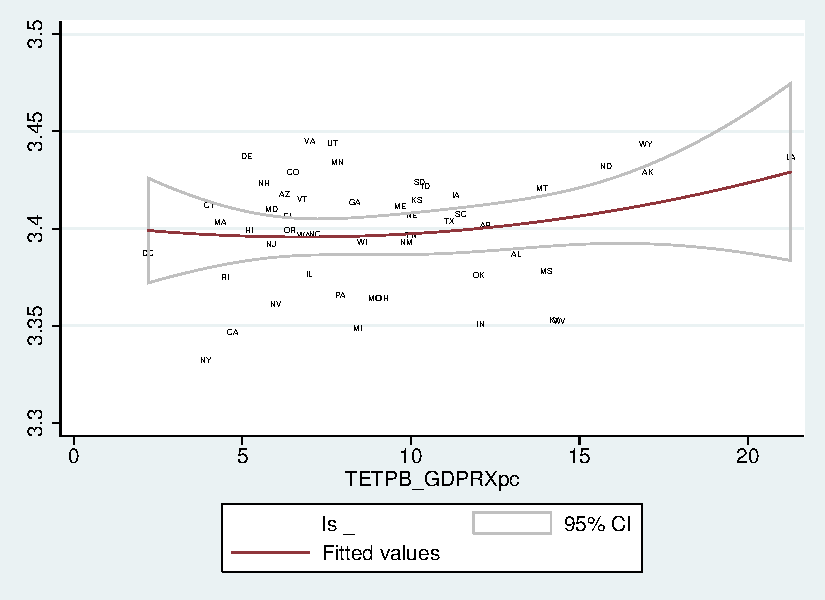
\includegraphics[width=6in]{graphsAndTables/lfTETPBgdpLS.pdf}\centering
\caption{Not much relationship here--note the scale of happiness--very small
  differences and much of that driven by WY, AK, and LA.}\label{lfTETPBgdpLS}
\end{figure}

\section{Over-time movement}

\begin{figure}[H]
 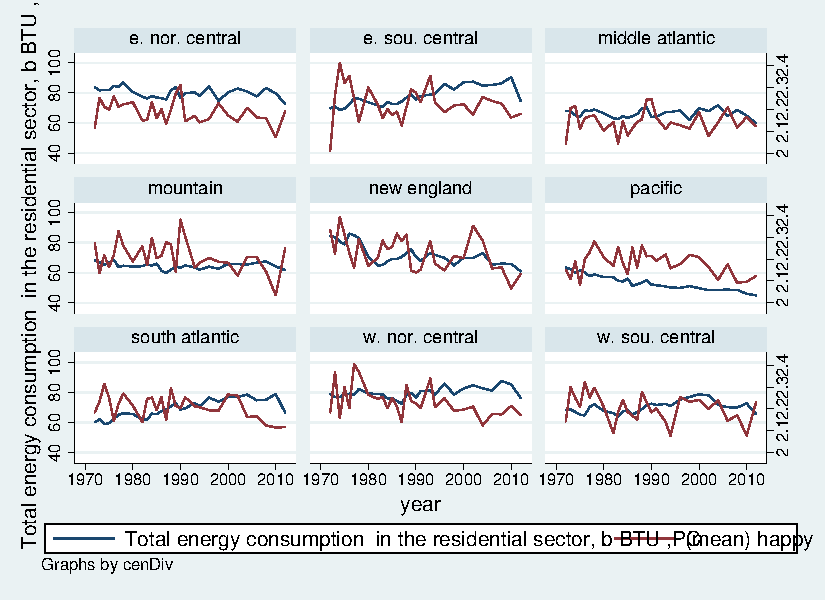
\includegraphics[width=6in]{graphsAndTables/cenDivLsYr.pdf}\centering
\caption{idea}\label{cenDivLsYr}
 \end{figure}

\begin{figure}[H]
 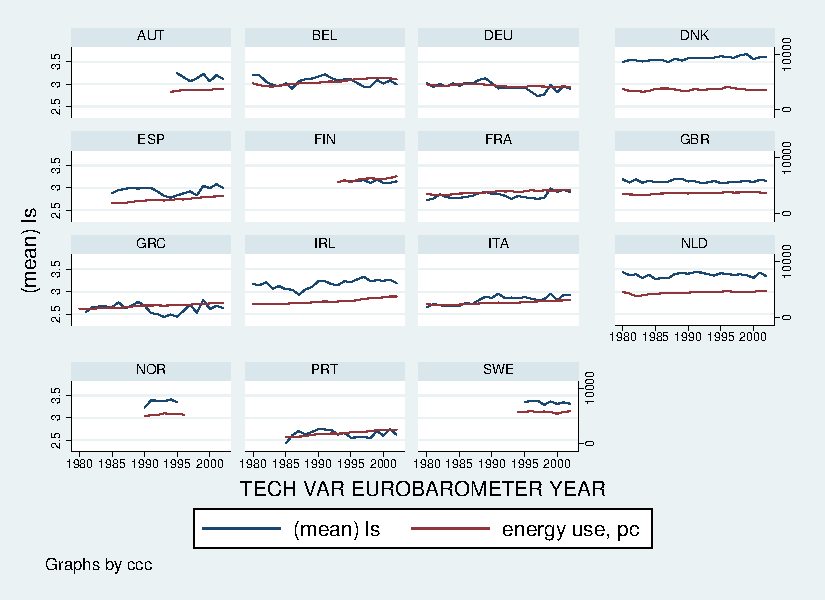
\includegraphics[width=6in]{graphsAndTables/ebTS.pdf}\centering
\caption{and over time not much relationship either !yet somehow corr is actually .5 }\label{ebTS}
\end{figure}


\section{Theoretical/conceptual additional information}

\subsection{What Do We Know So Far? The Literature}

% Micah -- We shouldn't set out to write a literature review. (No one should, except as part of a student thesis). The point is to put our findings in appropriate context. 
% Rely on the literature to establish 3 things:
% - the significance of the broad problem -- which should be supported by cites in the intro
% - that the problem being solved in the paper is important and hasn't been solved
% - that the rationale for the methods applied is sound

Energy use is getting more efficient due to technological imporvements and the
world economy is growing and hence every year we use less energy per gdp, but
still both energy use and co2 emissions, which correlate at above 90 percent,
are still growing every year \cite{iea14}. 


It is striking then that large happiness literature has omitted topic of energy
so far--threre are no studies about energy consumption and happiness across
areas, and only one study across persons.  \cite{graef81} (recently republished
as \cite{csikszentmihalyi14}) is the  only study about energy consumption and
happiness. This was a person-level study that used experience
sampling method (ESM) and it found no relationship between energy consumption
and happiness or even a negative relationship for females. 

% Micah: Few are stricken by the literature. What is striking is the universal assumption that
% consumption makes people happy, and the lack of any convincing empirical exampination of this claim.

Going back to initial question of how to achieve both happiness and
sustainabilty--we are not the first to try to answer it, we are only to fist to
do it using happiness and energy measures. Others used other measures.
Literature does look at the effect of energy consumption on human
wellbeing, but operationalizes human wellbeing differently--mostly as HDI or its
components. And literature proposes various indices linking HDI or its
components to natural resources or environment.

For instance, \cite{dietz09} proposed environmentally efficient wellbeing
(EWEB) as function of economic, natural and human resources. A simlar, but
closer to energy focus of present study is \cite{jorgenson14B} who proposed
energy intensity of human wellbeing. Yet, again, all of these approaches remain
in the realm of HDI or its components, GDP, education and life expectancy. 
 Using human development index (HDI) \cite{steinberger10} and argues along the
 same lines as present paper: increasing energy consumption beyond a point does
 not contribute anymore to wellbeing.  Many more studies link enrgy use to HDI
 \cite[e.g.]{dias06}, yet HDI, like  GDP, has its limitations--for an overview
 see \cite{klugman11}--and hence  recently happiness was proposed as another
 measure of broadly understood human  development--incidentally Amartya Sen both
 co-introduced HDI in 1990 and  reently advocatdes happiness \cite{stiglitz09al}. 

We will use happiness measure. But it is worth noting that there is also
 happy years measure (happiness$*$life expectancy) \cite{veenhoven96B}, and
 finally Happy Planet Index ($\frac{happiness*life\;expectancy}{ecological\;footprint}$)--this is somewaht close approach to  ours, except that we will try to see how energy consuption specifically afects  happiness. And there are few more: Genuine Progress Indicator, Ecological Footprints,  and planetary boundaries--see p. 477 in \cite{pretty13} for  sources. 

% Micah: The three paragraphs above are organized backward. State what we're doing first, then why we chose to do it, and what it adds to scientific knowledge. Don't ignore other work, but be positive.

While there is no literature about energy use and happiness, there is related
literature. \cite{pretty13} provides a wonderful overview of the relationship
betweenresource consumption, economy and wellbing including happiness measure of
it. There is literature about relationship between happiness and outcomes
related to energy consumption or attitudes about consumption. First, pollution makes us unhappy \cite{weinhold12,welsch05}. Second,
and more important,  there is some evidence that happy people
are more sustainable, that is, happiness affects sustainability
\cite{ericson14}.  Causation possibly goes in the
other direction as well (as noted by authors), but in general it is
safe to say that happiness and sustainable behavior are correlated  \cite{brown05,corral11}.

Then there is energy efficiency that moderaters (or mediates?) the relationship
between energy use and happiness--it is not only that energy use that results in
happiness, but importantly its efficient use--one country may waste lots of
energy say due to outdated and inefficent technologies as those in 1990s in
Eastern Europe, whereas some other ountry can actually use less energy per
capita but actually deliver more wellebing because enrgey is better used. We
will accounty for  energy efficiency by controlling for  $CO_2$ emissions. 
 A country that can produce more energy with less $CO_2$ is more energy
 efficient--perhaps a crude measure but readily available for a large sample of
 countries. There are better measures (e.g. \url{http://www.aceee.org/research-report/e1402}) but available for only a handful of countries
%can
                                %also do co2 per gdp  guess also can do co2 per
                                %energy etc etc

A related issue is that of ``rebound problem'' or the Jevons paradox
\cite{pretty13}%p476-477
--efficiency frees up resources that are then used to increase consumption, and
hence technological progress or efficient technology by itself does not lead to
sustainability. While in the developed World, energy consumption is flat or even
decreasing, it is globally increasing due to the developing World
\cite{pretty13}. Energy consumption, like economic growth and consmption has no
limit--indeed, instead of satysfying our needs it stimulates them--''the more
one has the more one wants, since satisfactions received only stimulate instead
of filling needs''   \cite{durkheim50}. This brings us to three major happiness
theories, all relevant to this study. 

% The three paragraphs above don't belong here. The appropriate time to introduce this information is to integrate it into the approach or discussion of interventions, to the extent this prior work is important for  what we should choose to measure, or for the design of appropriate interventions.



Before answering a question of how is happiness created, let's define it first. 
  Happiness, or the more scientific term Subjective Well-Being (SWB), is ``both cognitive judgments of one's life
satisfaction in addition to affective evaluations of mood and
emotions'' \cite[p. 142]{steel08},  or in other words: ``overall judgment of life that draws on two sources of information:
  cognitive comparison with standards of the good life (contentment) and
  affective information from how one feels most of the time (hedonic
  level of affect).''(\cite[p. 2]{veenhoven08})
 Some scholars make a
  distinction between happiness and life satisfaction--life
  satisfaction refers to cognition and happiness refers to affect. In practice,
  however, it is usually difficult  if not impossible to separate the two
  concepts.  Hence, the overall happiness definition by 
   \cite{veenhoven08}, as quoted above,  seems most appropriate and we will use terms
   ``happiness,''``life satisfaction'' and ``(subjective) wellbeing'' interchangeably.  For a recent and very through statement of
happiness measure validity and reliability see \cite{diener09}
(especially ch. 5). 

% Micah: Explain why this is the best way of defining happiness for the purposes of understanding energy consumption.
There are many ways to measure human wellbeing. Traditionally, we have used
income measures such as per capita gross dometic product or health measures such
as life exectancy or human development measures such as education. %HDI index 
 It has been recognized recently, however, that these measures do not capture
 human wellbeing well--two key problems are that these measures are not
 comprehensive enough and it is difficult to combine them into a single measure
 because weights are always arbitrary. The co-inventor of the original
 development metric (Human Development Index), Amartya Sen, has recently
 proposed happiness as a better measure \cite{stiglitz09al}.

\subsection{The three happiness theories}
The adaptation theory \cite{brickman78cj} argues that there is
adjustment to external circumstances and we are on a 'hedonic
treadmill.' ``The more one has the more one wants, since satisfactions
received only stimulate instead of filling needs''\cite{durkheim50}. 
We arguably get used to (adapt to) energy consumption, too. Hence, increasing
energy consumption is futile for our happiness, because we will adapt to it and
always want more.
%
The  multiple discrepancy theory  \cite{michalos85} states that
happiness is a result of social comparison or a comparison to various
standards.  I compare my consumption to others. I also compare
it to standards--for instance, that of people in my geographic or social
proximity. Notably, this may result in consumption arms race--people wanting to
outcompete others in terms of consumption in a vicious
cycle \cite{frank12}. Hence, also like  per adaptation theory, energy consumtion
will not result in geater happiness.  
%
  The needs/livability theory \cite{veenhoven95, veenhoven14b} posits that
  happiness results from objective living conditions and from
  fulfillment of our needs, and predicts that higher physical or economic
  development will result in greater happiness. It is not clear, however, if
  there is any limit to the level of development that should result in greater
  happiness as it is not clear what is the limit to human needs. Of course, one
  could argue that there are needs and wants, and while there are some clearly
  defined needs (e.g. biological), most other needs are relative and
  subjective. Hence, based on this theory, as opposed to the other two theories,
  greater energy use will result in greater happiness.
  
\subsection{Future Research}

TODO set research agenda somewhare!! for future research!

There are many ideas for future research. Indeed, as mentioned earlier, one of
the goals of this study is to encourage more research on this important and
overlooked topic of energy consumption and happiness.

We just examined total energy use per capita at country level without
differentiating between sectors, because we could not find ssuch data. There are
however enrgy use data by sector for smaller sets of countries--for instance for
Europe available from Eurostat: 
\url{http://epp.eurostat.ec.europa.eu/portal/page/portal/energy/data/database}, \url{http://epp.eurostat.ec.europa.eu/portal/page/portal/energy/data/main_tables} 

We suggest that clean energy would result in greater happiness. This idea could
poissibly be tested more direcly by examining happiness of people in areas where
clean energy is prevalent. 


Yet, energy efficiency or even clean energy is not the final solution due to
``rebound problem'' or the Jevons paradox--due to innate human greed we are
likely to consume ever more and more, and hence the only lasting solution is to
curb our energy hunger possibly through public policy and education.


\subsection{Comparability of Results}

We did not make same scales on graphs for reason of interpretaility. We could
make both scales, happiness and energy standarized, but then it is more
difficult to intepret results, we think. In this approach, we have followed
\cite{easterlin10B,easterlin12}, who also used different unstandarized
happiness scales in the same study. 



\newpage
\section{\huge OLD/OTHER/EXPERIMENTAL STUFF: just for us, not to be summitted} initially in another document: graphsAndTables.tex

\section{most current stuff}

\ref{couWvsLsEleHHgdp} shows Average electricity consumption per electrified household, kWh, from World
Energy Council (1990-2011) (\url{http://www.wec-indicators.enerdata.eu/household-electricity-use.html}), which are also averaged. 
% energy use from World Bank (\url{http://data.worldbank.org/indicator})
   US consumes
in its residential sector about more than 3 times the median.%sum eleHH
                                %if yr==2011 & c=="USA", det for FULL sample 
From first panel, it appears
 as if there is a positive relationship, but it is simply due to wealth. Simply,
 developed countries consume more energy than developing countries, and we know
 that in a cross-section, wealthier countries are happier. The second panel
 measures on x-axis energy intensity of gross domestic product (GDP)
 (energy/GDP). Here, the relationship is opposite--countries that  consume less
 energy per unit of wealth are happier. In other words, the less energy use
 given income level, the more happiness. We speculate that to acheive greater happiness we
 do not necessarily need to increase GDP keeping energy constant; we could stop
 growing GDP and decrease energy use. For instance, the Netherlands (NLD) is
 happy, developed and energy efficient. China (CHN) is developing and medium
 happy, but consumes more energy per GDP than developed and happier USA does.  
Latin America countries, pose a puzzle for happiness researchers-they are
relatively poor and yet quite happy, but they also  use very liitle  energy per
their GDP and have simialr energy inetsity of GDP as the US. Next, we zoom in on
US states and counties.
% also see http://www.ritholtz.com/blog/2010/06/oil-consumption-around-the-world/ 

\begin{figure}[H]
 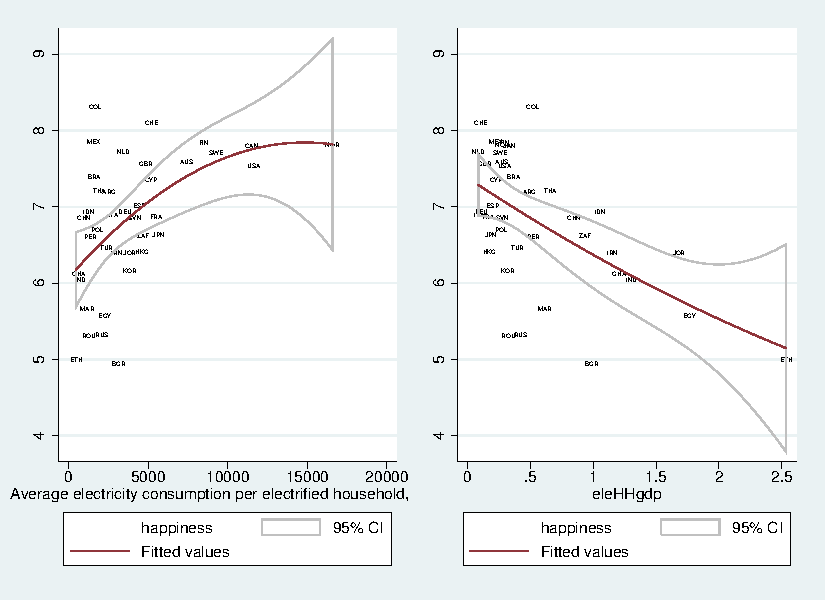
\includegraphics[width=6in]{graphsAndTables/couWvsLsEleHHgdp.pdf}\centering
 \caption{Happiness against average electricity consumption per electrified
   household, kWh.}\label{couWvsLsEleHHgdp}
\end{figure}
{\scriptsize Note: Country codes are in table \ref{ls} in supplementary
  material. If country was observed in more than one year, the data were averaged.}



Well, true energy look positive, but so what ! does it mean more energymore
happiness. no. it is quadratic!!! so it levels off at around 4k of energy
use--beyond that anergy use does not seem to help much wiuth happiness; like
with income--it also levels off at country or regional levble (my paper!)

it is interesting that the ere is positive quadratic relationship in rich
countries and negative in poor countries...the cutoff point is at 10k of pcgdp.

note: happiness and gdp were averaged over time: in wvs there are couple years;
in mannheim there are 30years so not sure if averaging is a great idea in
mannheim; but if each country-year plotted, it's quadratic also 


\begin{figure}[H]
 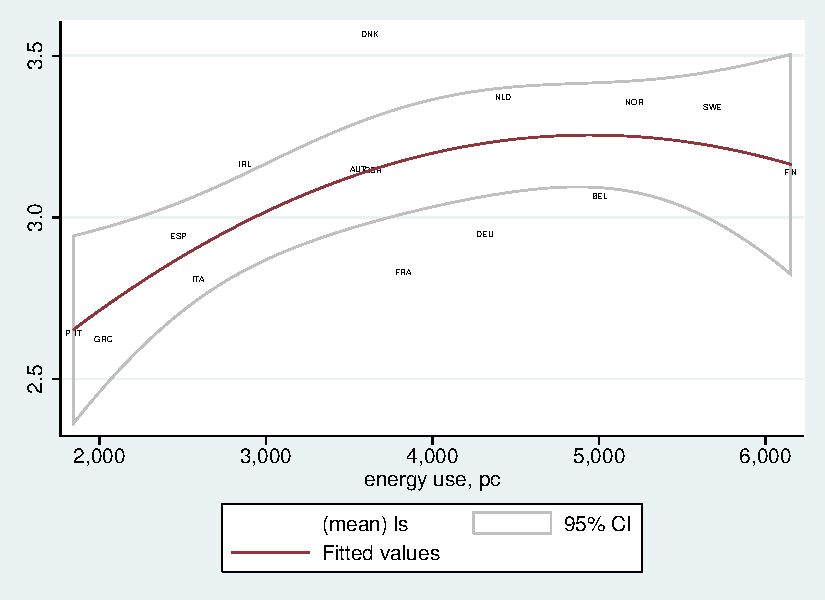
\includegraphics[height=3in]{graphsAndTables/couLsEne.pdf}\centering
\caption{couLsEne.pdf Eurobarometer dataset for west european (rich countries)}\label{couLsEne.pdf}
\end{figure}
{\scriptsize Note: Country codes are in table \ref{ls} in supplementary
  material. If country was observed in more than one year, the data were averaged.}

\begin{figure}[H]
 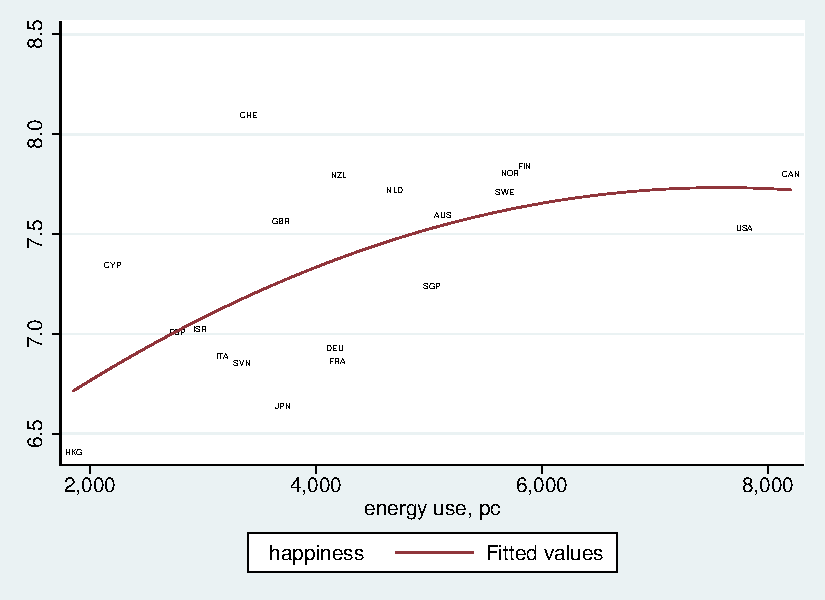
\includegraphics[height=3in]{graphsAndTables/couWvsLsEne.pdf}\centering
\caption{World Values Survey Data data; countries$>$10k pcgdp couWvsLsEne.pdf}\label{couWvsLsEne.pdf}
\end{figure}
{\scriptsize Note: Country codes are in table \ref{ls} in supplementary
  material. If country was observed in more than one year, the data were averaged.}


\begin{figure}[H]
 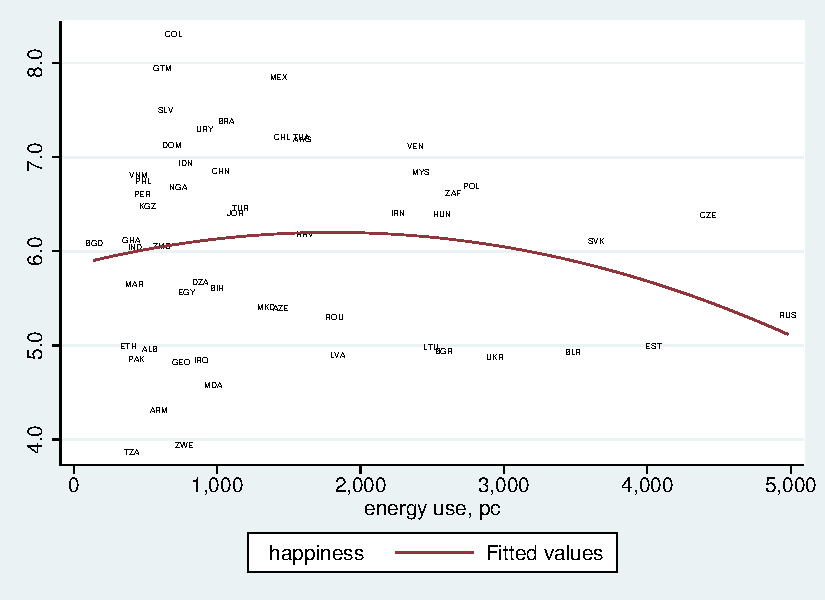
\includegraphics[height=3in]{graphsAndTables/couWvsLsEneLT10kGDP.pdf}\centering
\caption{couWvsLsEneLT10kGDP.pdf World values survey data country level for
  countries lt 10k pcgdp--btw this doesn't make sense--should be the other way
  round--more ebergy consumption is helpful in poor countries, not rich onese
  e.g. as per \cite{mazur11}}\label{couWvsLsEneLT10kGDP.pdf}
\end{figure}
{\scriptsize Note: Country codes are in table \ref{ls} in supplementary
  material. If country was observed in more than one year, the data were averaged.}


\begin{figure}[H]
 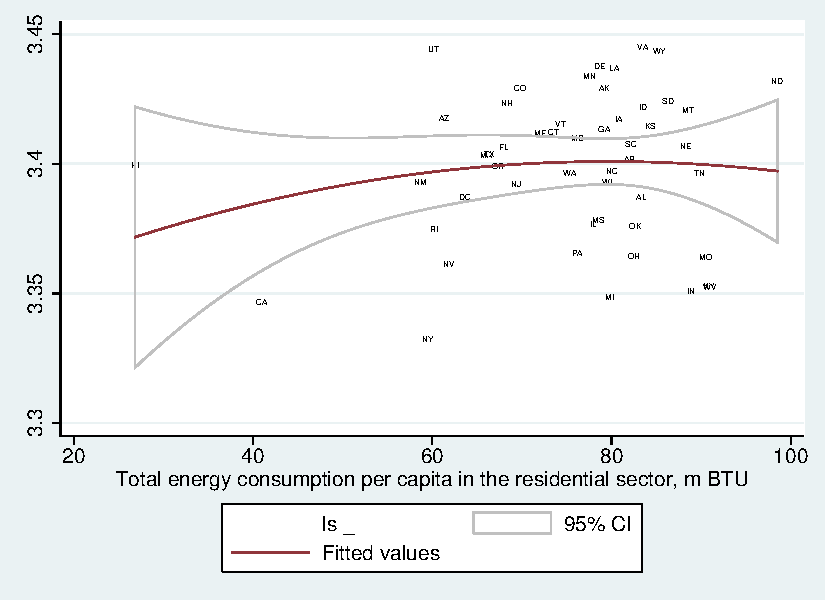
\includegraphics[height=3in]{graphsAndTables/lfTERPBls.pdf}\centering
\caption{lfTERPBls.pdf residential energy consumptionm; no relationship here !
  except that hawaii is warm and doesn't consume much and california is green!
  so now zooming in on california :)}\label{grComTETPBgdp}
\end{figure}
{\scriptsize TODO Note: Country codes are in table \ref{ls} in supplementary
  material. If country was observed in more than one year, the data were averaged.}


\begin{figure}[H]
 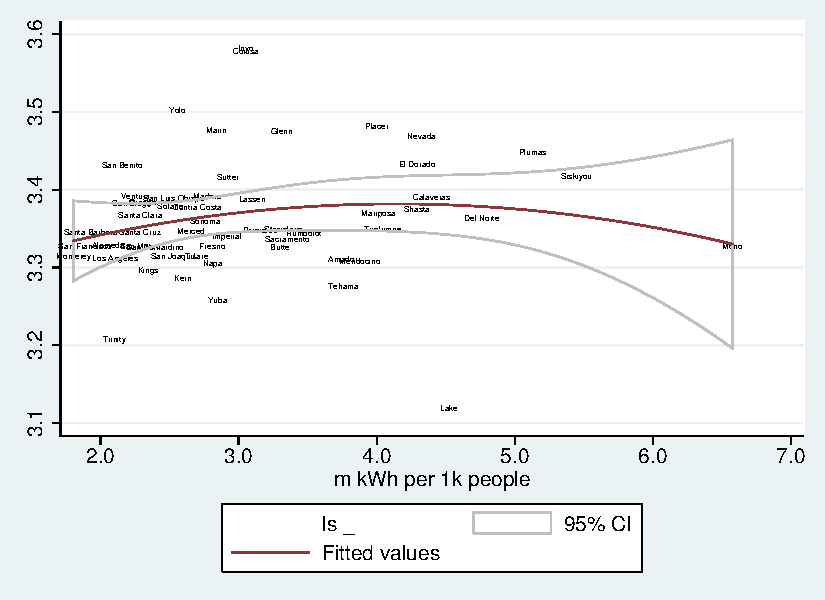
\includegraphics[height=3in]{graphsAndTables/lfELERESls.pdf}\centering
\caption{residential energy use; nothing reallyu here...wonde why Mono uses so much!}\label{}
\end{figure}
{\scriptsize TODO Note: Country codes are in table \ref{ls} in supplementary
  material. If country was observed in more than one year, the data were averaged.}

\begin{figure}[H]
 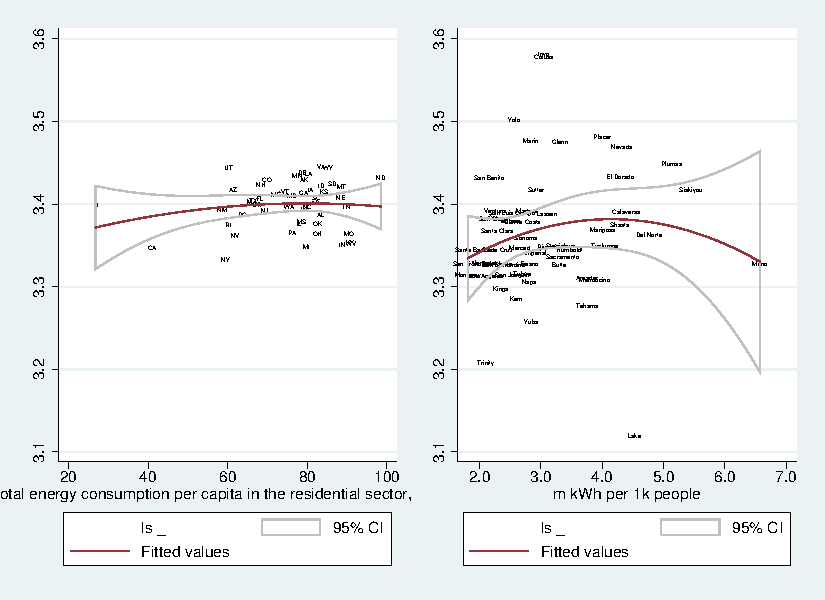
\includegraphics[width=6in]{graphsAndTables/stateCa.pdf}\centering
\caption{WVS all countries, avergaed over time;; in this second step we explore
at state and county lev and nothing there whether with or without gdp--and
importantly as at ctry lev also energy intencsity attenuates slope albeit much
less dramatcally}\label{stateCa}
 \end{figure} {\scriptsize Note: Country codes are in table \ref{ls} in supplementary material. If country was observed in more than one year, the data were averaged. }


\subsection{Energy intensity of gross domestic product (GDP) (energy/GDP)}

\url{http://en.wikipedia.org/wiki/Energy_intensity}:
High energy intensities indicate a high price or cost of converting energy into GDP.
 
\begin{figure}[H]
 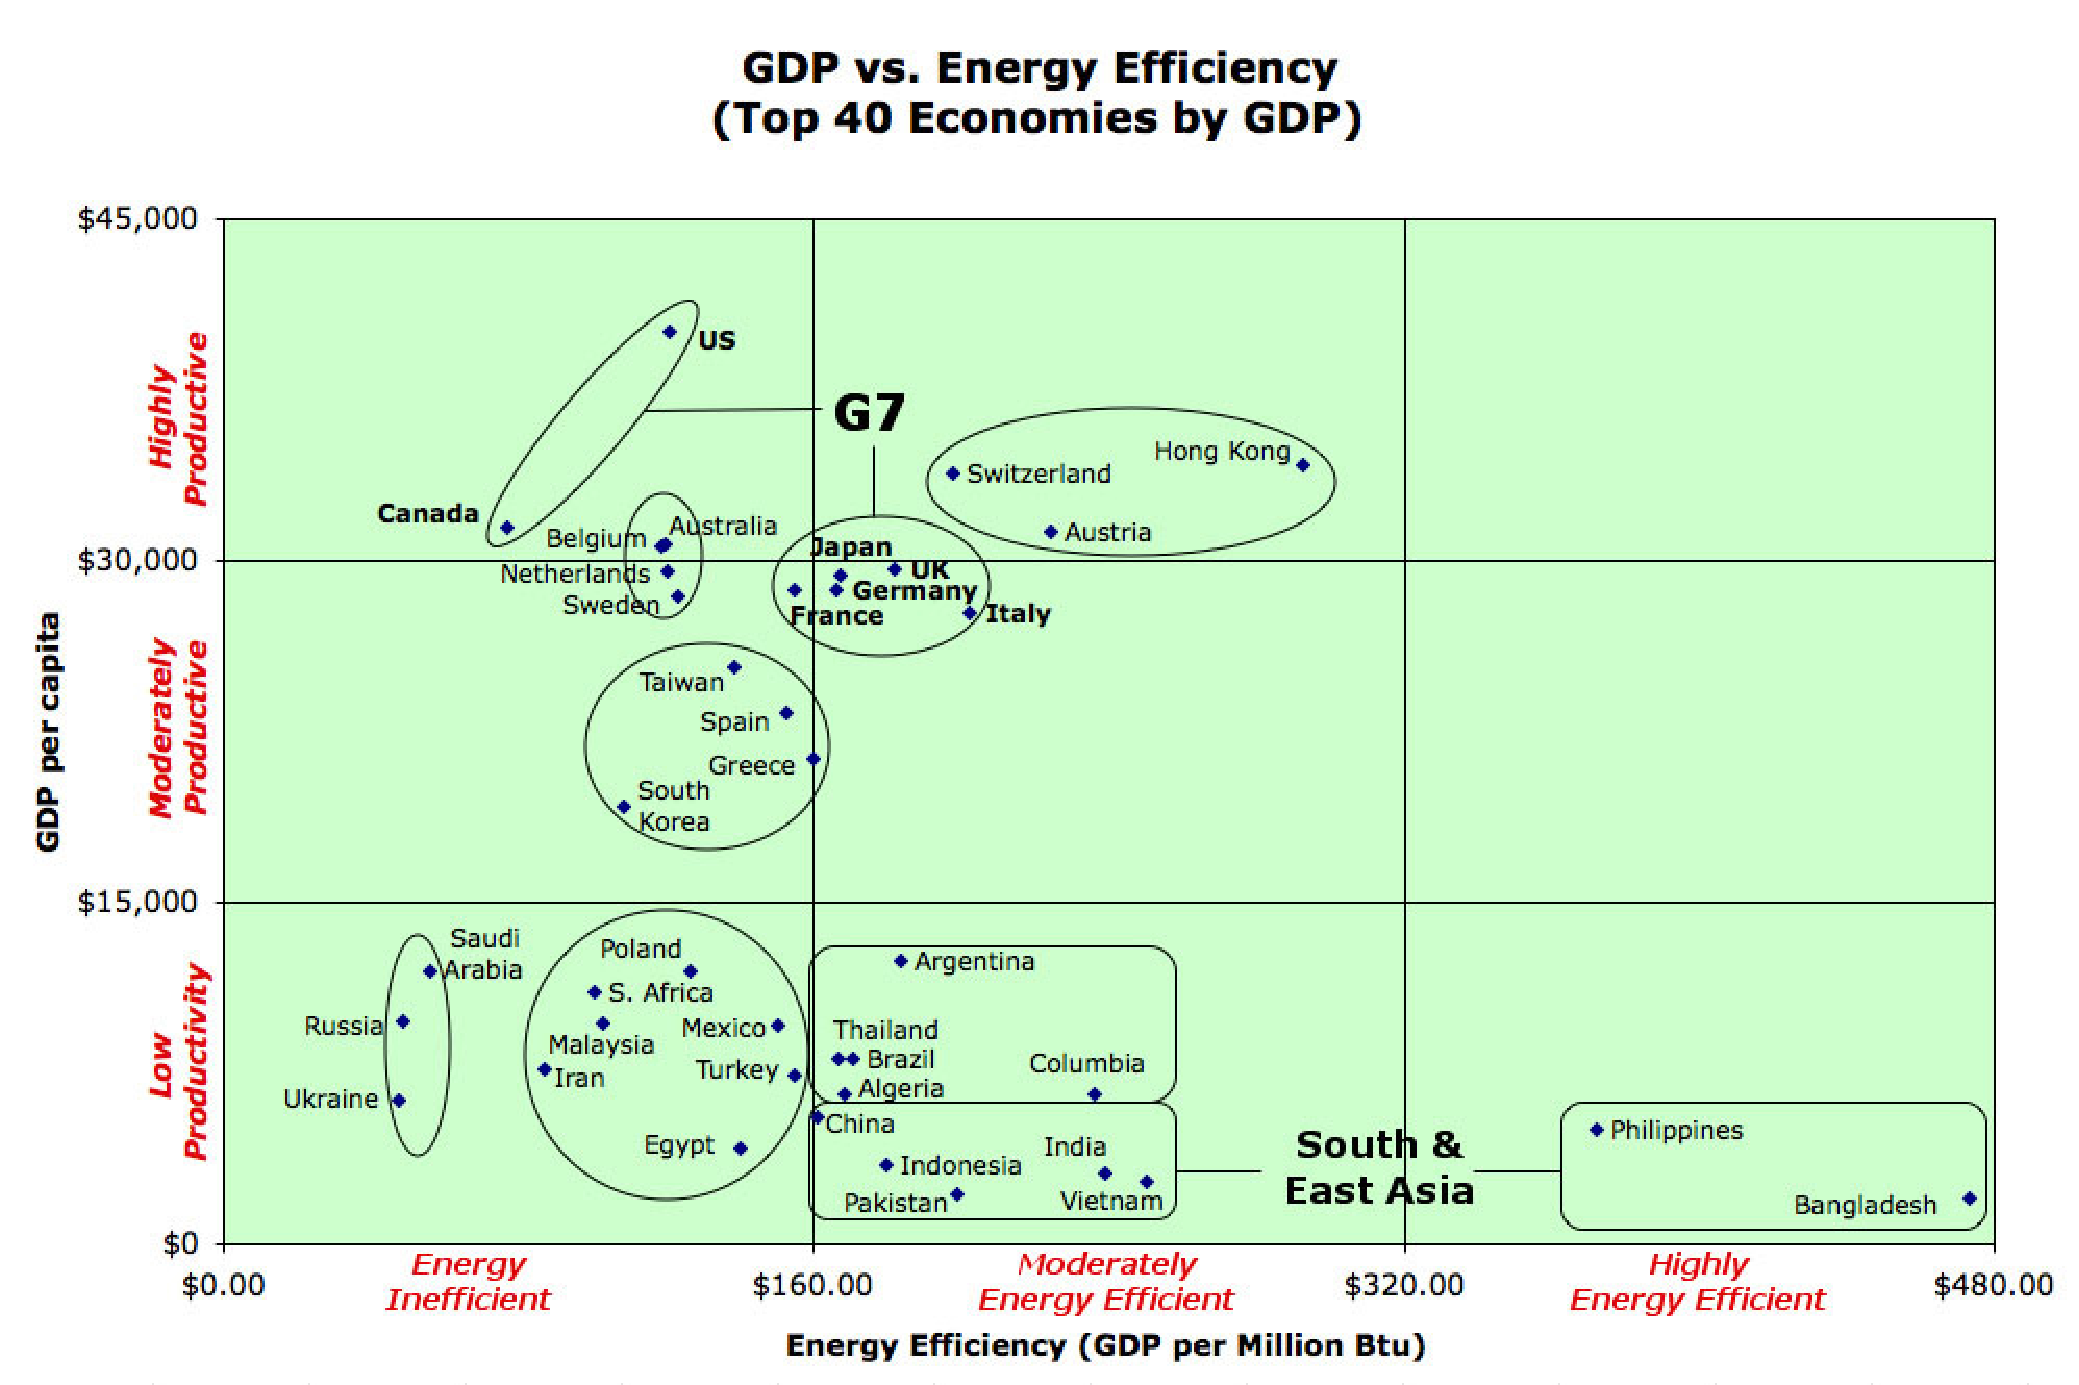
\includegraphics[height=5in]{graphsAndTables/Gdp-energy-efficiency.pdf}\centering
\caption{a cool graph from wikipedia :)}\label{}
\end{figure}
and can also use energy intensity PPP adjusted--see above wikipedia article and \url{http://en.wikipedia.org/wiki/List_of_countries_by_energy_intensity}

There is not much relatyionship between happpiness and energy use, but there is
even less if controlling for GDP--energy use correlates with GDP and it if nit
controlling for GDP then it proxies it and then results are spurioius and what
we see is the effect of GDP, not energy use.  
To alleviate that problem we could have controlled for GDP. But we can do it
another way, too. 
Another way to look at it is to use so called energy intensity of gross domestic
product (GDP): (energy/GDP). Below  are graphs doing just that.


\begin{figure}[H]
 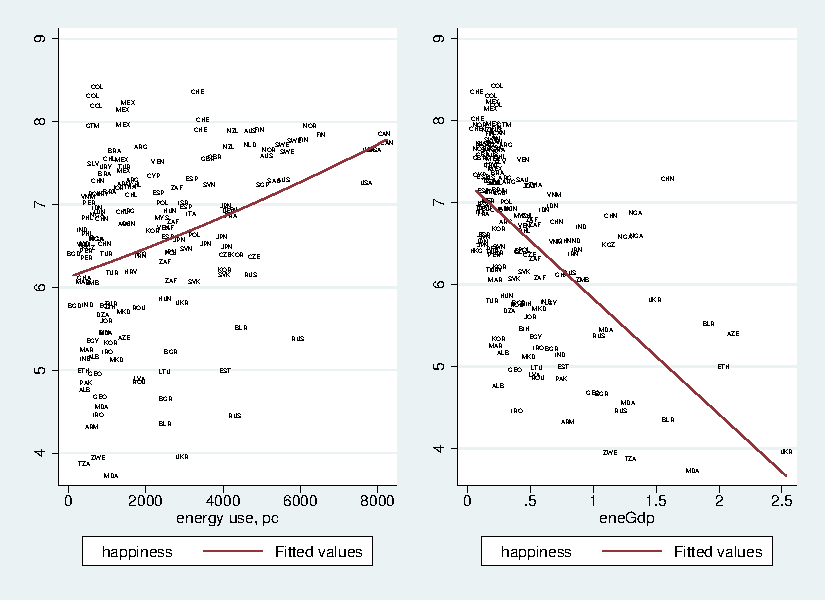
\includegraphics[height=3in]{graphsAndTables/couWvsGrComEneGdp.pdf}\centering
\caption{couWvsGrComEneGdp}\label{couWvsGrComEneGdp}
\end{figure}
{\scriptsize Note: Country codes are in table \ref{ls} in supplementary
  material. If country was observed in more than one year, the data were averaged.}

latin american ctries like COL or MEX very little energy per gdp; while post
soviet like ukraine or MDA BLR AZE ARM are very energy intesive and miserable

What is striking is the differences in energy use by area. Diferences are
severalfold. Mexico and Colombia
consume only ??? and yet are as happy as ??? which consumes ???.

\begin{figure}[H]
 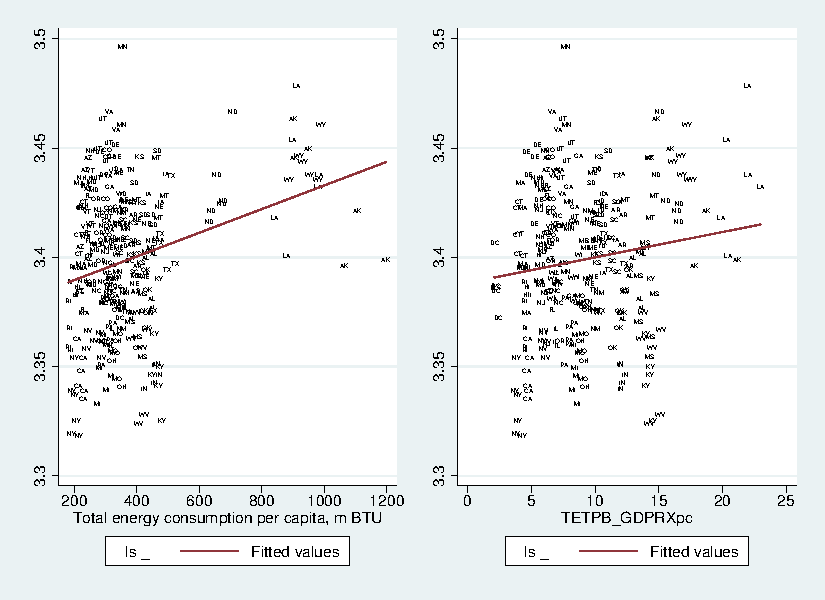
\includegraphics[height=3in]{graphsAndTables/grComTETPB_gdp.pdf}\centering
\caption{grComTETPBgdp}\label{grComTETPBgdp}
\end{figure}
{\scriptsize TODO Note: Country codes are in table \ref{ls} in supplementary
  material. If country was observed in more than one year, the data were averaged.}

for states teh positive results are divern only by LA, ND, WY, AK; othersie
nothing there, can do a graph dropping those

\begin{figure}[H]
 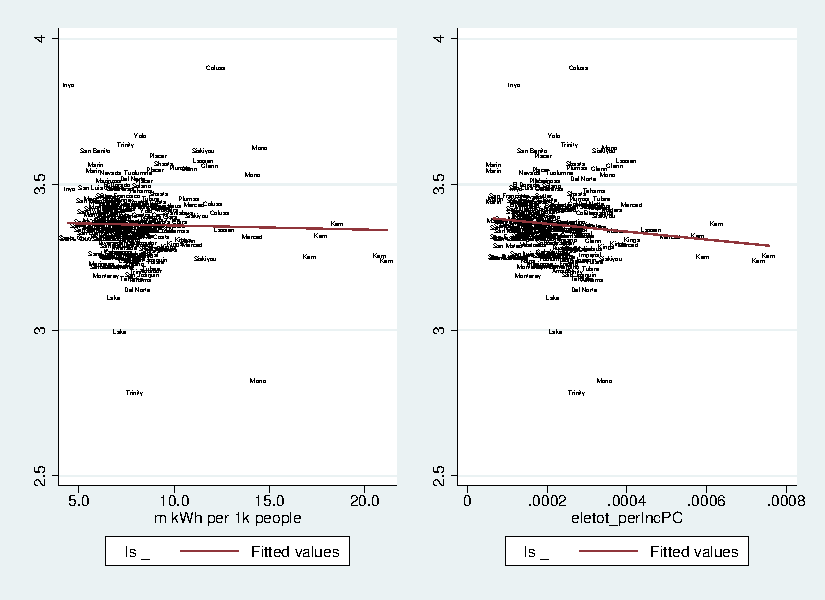
\includegraphics[height=3in]{graphsAndTables/eletot_gdp.pdf}\centering
\caption{eletotgdp}\label{eletotgdp}
\end{figure}
{\scriptsize Note: Country codes are in table \ref{ls} in supplementary
  material. If country was observed in more than one year, the data were averaged.}

%note: cen div is somewhat weird...


so need to have more gdp, less energy use, at least across countries...


What is striking is the differences in energy use by area. Diferences are
severalfold. Mexico and Colombia
consume only ??? and yet are as happy as ??? which consumes ???.


\begin{figure}[H]
 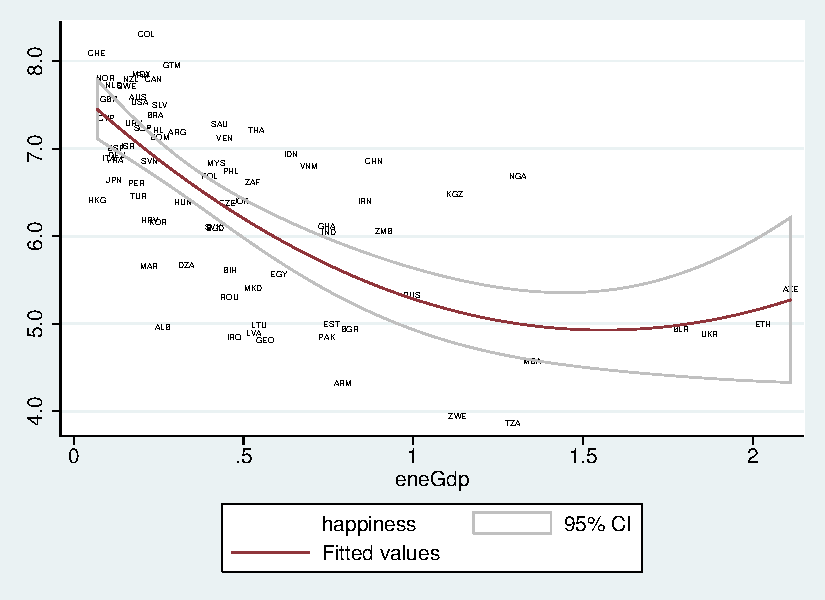
\includegraphics[height=3in]{graphsAndTables/couWvsLsEnePerGdp.pdf}\centering
\caption{total energy use divided by gdp}\label{}
\end{figure}
{\scriptsize TODO Note: Country codes are in table \ref{ls} in supplementary
  material. If country was observed in more than one year, the data were averaged.}

\begin{figure}[H]
 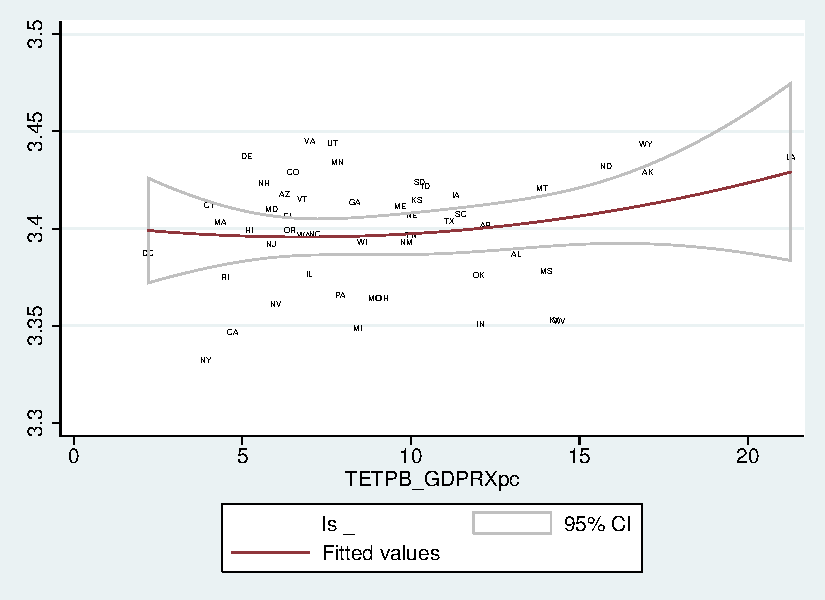
\includegraphics[height=3in]{graphsAndTables/lfTETPBgdpLS.pdf}\centering
\caption{total energy use divided by gdp}\label{}
\end{figure}
{\scriptsize TODO Note: state codes are in table \ref{ls} in supplementary
  material. If country was observed in more than one year, the data were averaged.}

\begin{figure}[H]
 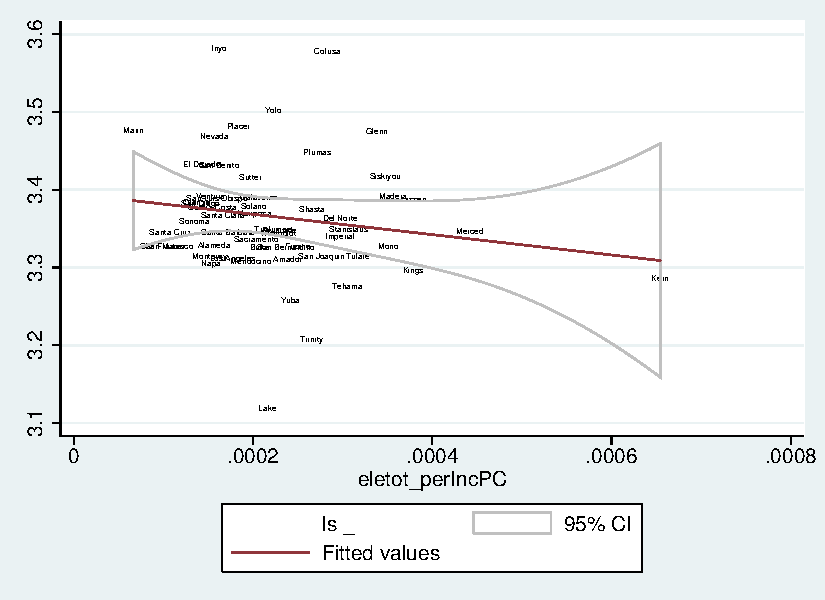
\includegraphics[height=3in]{graphsAndTables/caEleTotGdp.pdf}\centering
\caption{total energy use divided by gdp}\label{}
\end{figure}
{\scriptsize TODO Note: Country codes are in table \ref{ls} in supplementary
  material. If country was observed in more than one year, the data were averaged.}

\begin{figure}[H]
 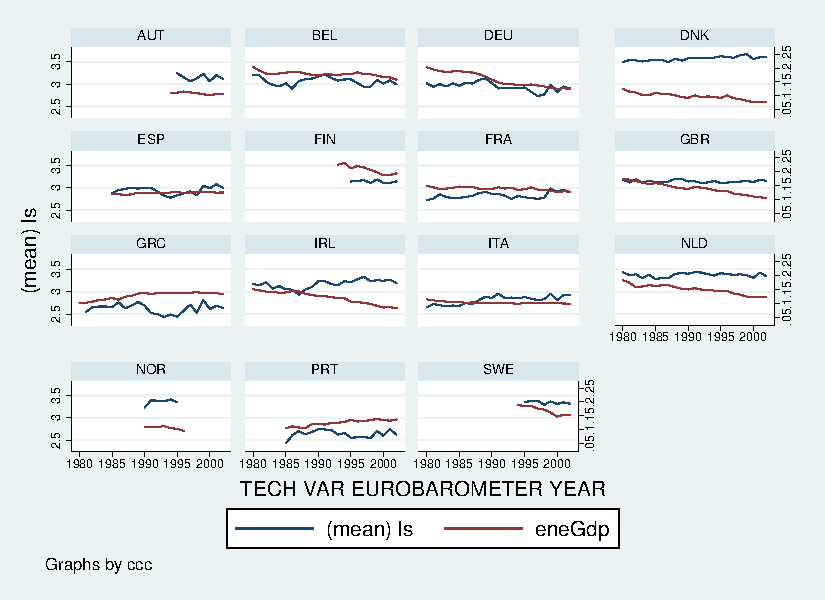
\includegraphics[height=3in]{graphsAndTables/ebTSeneGdp.pdf}\centering
\caption{happiness and (total) energy intesity of gdp}\label{ebTSeneGdp}
\end{figure}

\begin{figure}[H]
 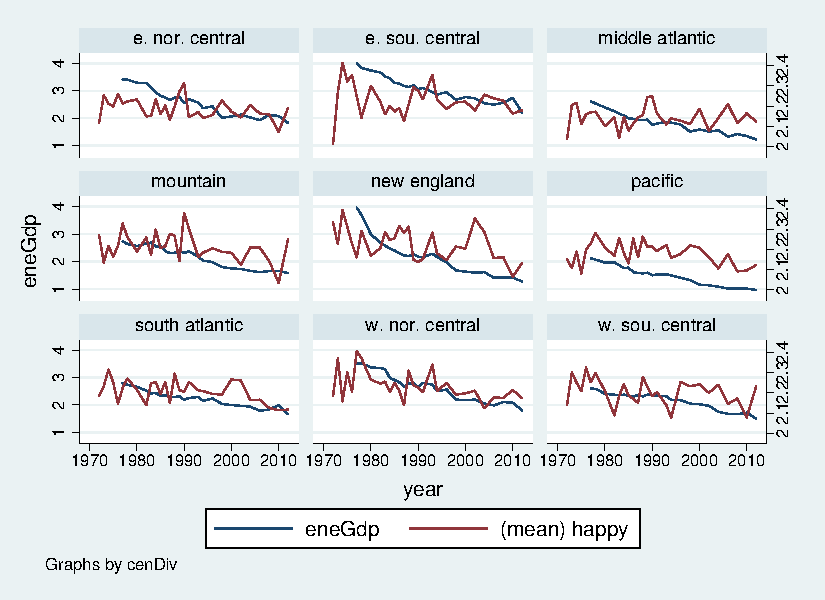
\includegraphics[height=3in]{graphsAndTables/cenDiveneGdp.pdf}\centering
\caption{happiness and (residential) energy intesity of gdp}\label{cenDiveneGdp}
\end{figure}

maybe this approach in gigures \ref{cenDiveneLs} and \ref{ebTSeneLs} is a way to
go--we have energy intesity of gdp so maybe do energy intesity of happiness!
especially that Sen recently adocated to use happiness to measure progress.

\begin{figure}[H]
 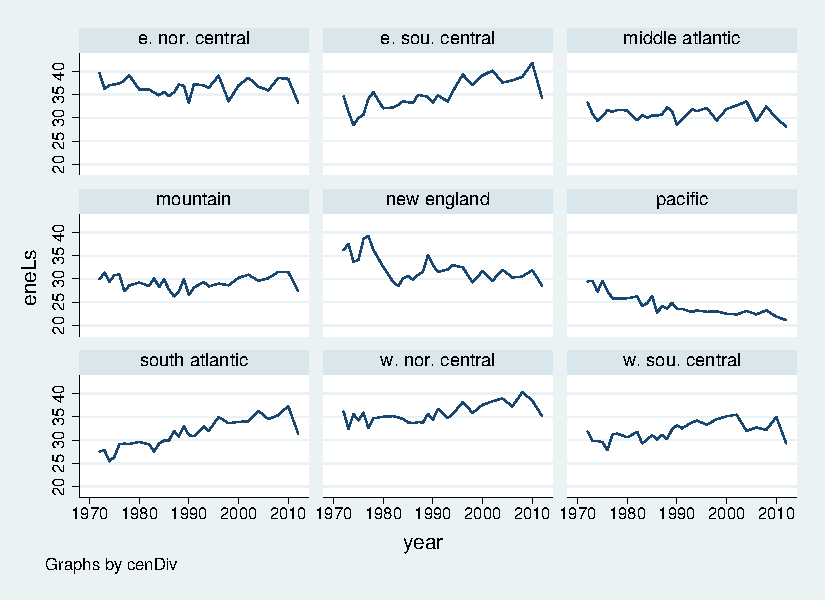
\includegraphics[height=3in]{graphsAndTables/cenDiveneLs.pdf}\centering
\caption{happiness and (residential) energy intesity of happiness--Pacific is
  doing great--maybe Green California? While East is considerably worse! }\label{cenDiveneLs}
\end{figure}

\begin{figure}[H]
 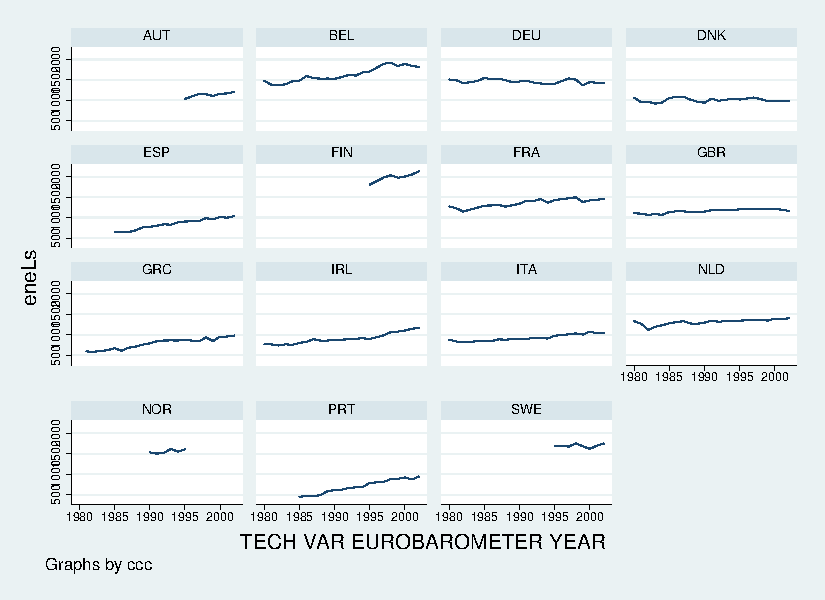
\includegraphics[height=3in]{graphsAndTables/ebTSeneLs.pdf}\centering
\caption{Europe is getting worst and worst; Northern Scandinavian countries
  worse--arguably because it is cold tehre, while Southern are lower}\label{ebTSeneLs}
\end{figure}

\subsection{multivariate: other things}
\label{mvarOthThings}

So how come there is not much in bivariate relationship except in the
World--well as already hinted at in that first figure, there are other things
going on, like GDP that we controlled for in that figure, adn so we would
explore some of those things here. At the same time, this section sets the stage
for the future research and explores a bit some of those ideas.
\textbf{TODO:} can discuss here some loiterature as i guess i had it earlier at
the beginning in tghe literature review and then removed to that other pdf file...


And we also take into accouint more factors in the regressions framework in the
online appendix

\begin{figure}[H]
 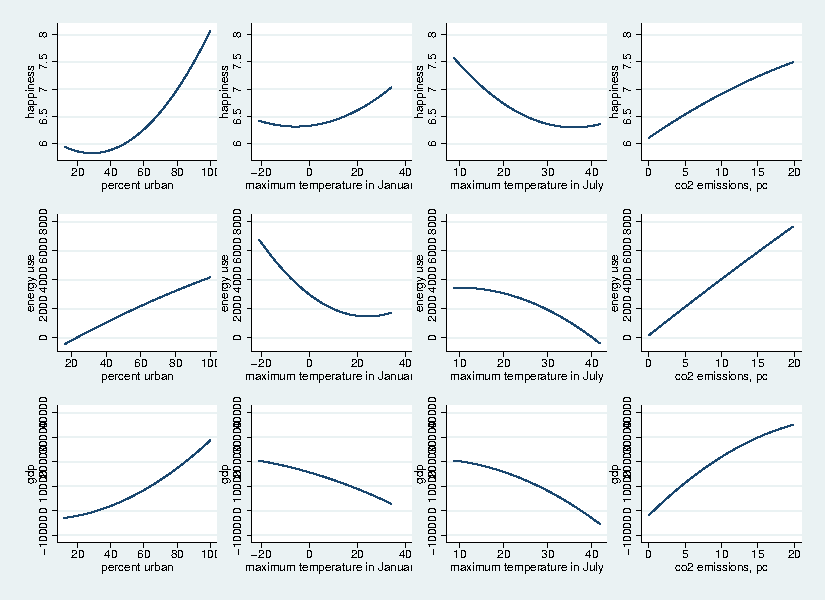
\includegraphics[width=6in]{graphsAndTables/mat1.pdf}\centering
\caption{id: mat1;  note that this is total energy, not residential, and it is not avergaed
over yrs}\label{mat1}
 \end{figure}


\subsubsection{multivariate: other things:: but gasoline consumption is good !}

well, driving may be result of happiness: happy people go places; miserable
folks stay home and watch tv; and may reflect overall mood of the
place--activity or even business cycle i guess

\begin{figure}[H]
 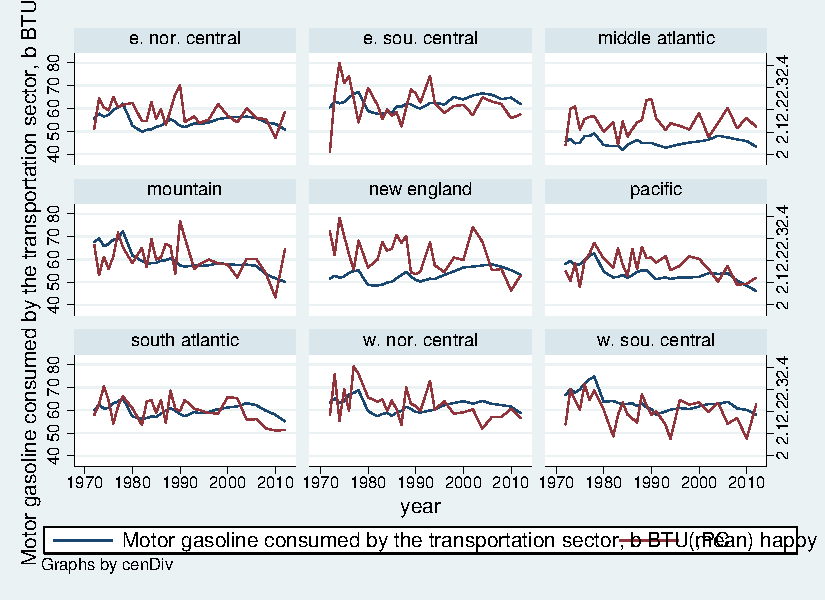
\includegraphics[width=6in]{graphsAndTables/cenDivLsYrMGAPB.pdf}\centering
\caption{but driving is good !}\label{cenDivLsYrMGAPB}
 \end{figure}

\subsubsection{multivariate: other things:: but natural gas consumption is good !}

\begin{figure}[H]
 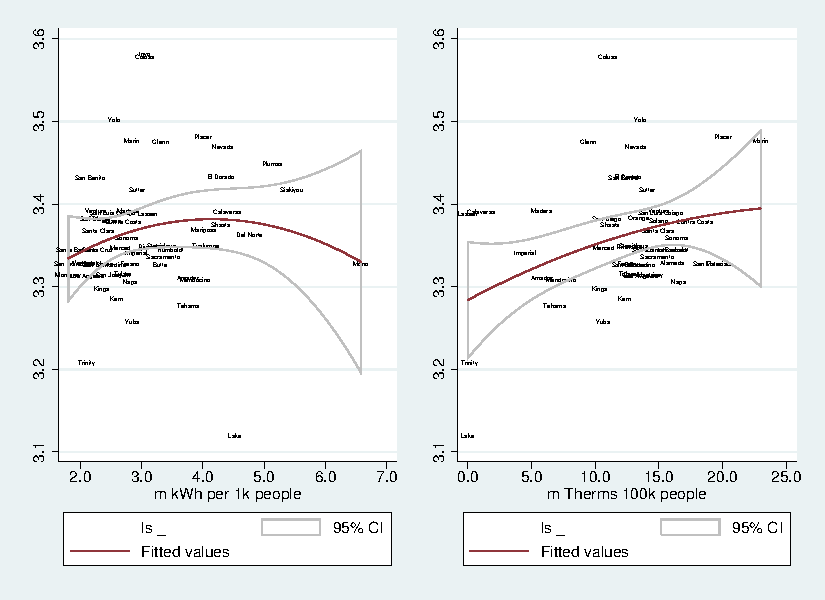
\includegraphics[width=6in]{graphsAndTables/caEleGas.pdf}\centering
\caption{driving is good in california as well ! (left electrisity; right gas)}\label{cenDivLsYrMGAPB}
 \end{figure}

\subsubsection{multivariate: other things:: breaking it down by other things: hi--lo}

\begin{figure}[H]
 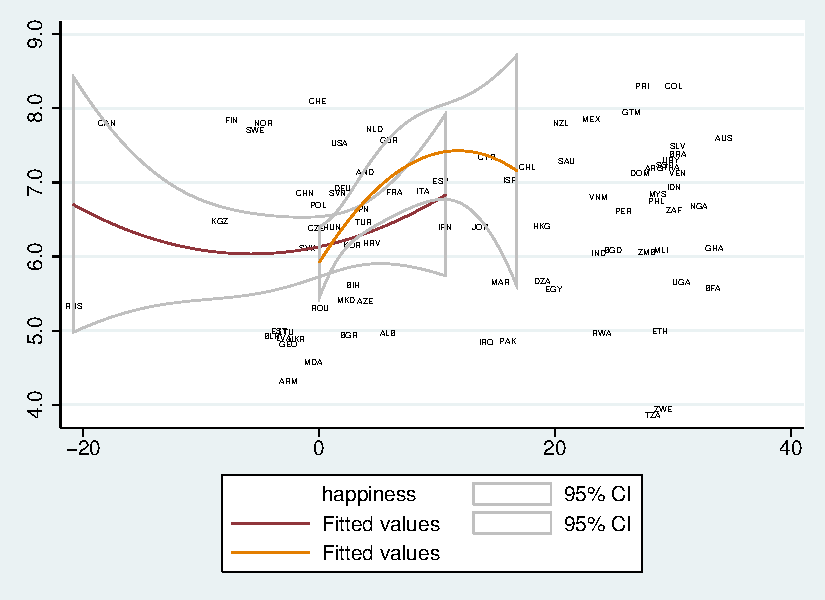
\includegraphics[width=6in]{graphsAndTables/co2twice.pdf}\centering
\caption{}\label{cenDivLsYrMGAPB}
 \end{figure}

\begin{figure}[H]
 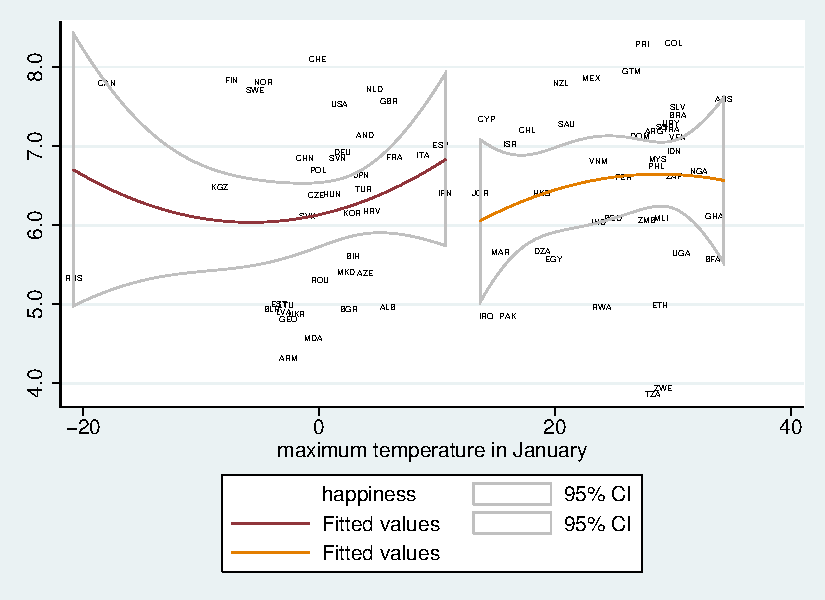
\includegraphics[width=6in]{graphsAndTables/JanTwice.pdf}\centering
\caption{}\label{JanTwice}
 \end{figure}

\begin{figure}[H]
 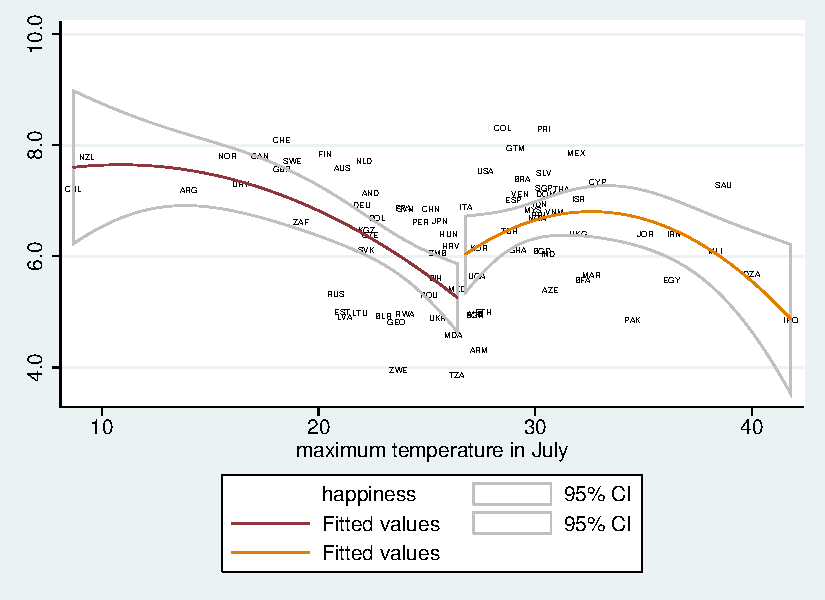
\includegraphics[width=6in]{graphsAndTables/JulTwice.pdf}\centering
\caption{}\label{JulTwice}
 \end{figure}

\begin{figure}[H]
 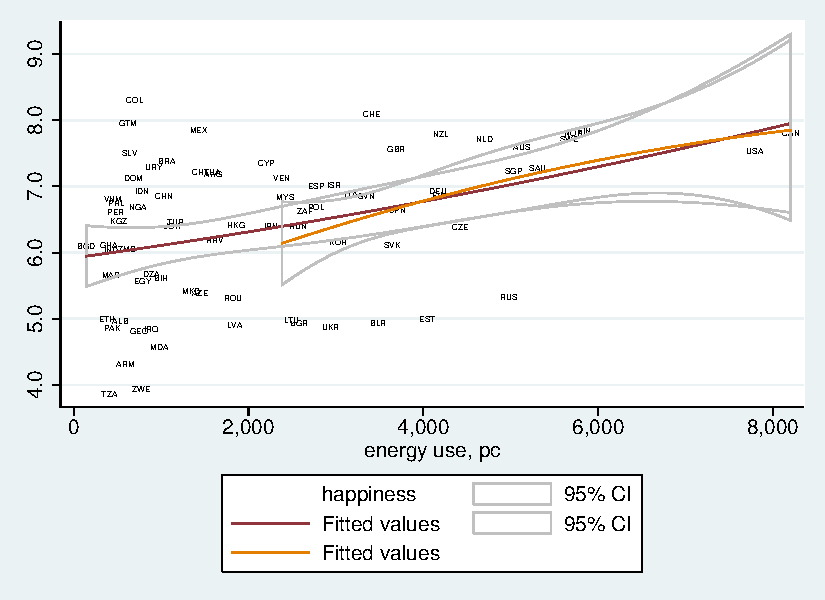
\includegraphics[width=6in]{graphsAndTables/eneTwice.pdf}\centering
\caption{}\label{eneTwice}
 \end{figure}




\section{What is Wrong With Texas?}

There are obviously many things wrong with Texas, but we would like to focus on
consumption, energy use, eceonomic development in general and envrionment. They
say that ``everything is big in Texas,'' 

This paper was born on the Sprit\footnote{Author is a social scientist and
  cannot afford non-frugal airlines.} flight 215 approaching DFW airport. I am
flying PHL-DFW every month and always wonder about energy use when I approach
Dallas. From the airplane you see big roads and huge highways connecting bi
houses (so called McMansions) with huge shopping areas. And you see big cars and
in them big Texans (Texans are not big enough yet to spot them from the
airplane, but you'll see them once you land). I though rom he airplane, geez,
they must use twice as much energy as on east coats, and checked data adn bingo
! they do about 2x (TODO gve exact numbers). 
Texas economy is growing fast but its open land is shrinking fast, too--and you
can see that from the airpplane, too--there is a sea of concrete as far as eye
can see; and there is some fake nauture constantly tended by Mexicans who use
more energy to cut grass and sweep with those air blowers. But numbers say the
same--Texas lost about 1.1 million acres between 1997 and 2012. 
\cite{marshallCL14}


\section{General Considerations}

\subsection{Electricty use: residential and non-residential} 
How is electricity used in United States homes? This is an important
consideration because it really shows what we do with this electricity--how we
consume it, what are the end uses. Data are shown in table
\ref{eleEndUse}. Furthermore end uses of energy changed over time, for instance
 from 1993 to 2009: applianes share increased from 24\% to 35\% and space
 heating dropped from 53\% to 41\%
 \url{http://www.eia.gov/todayinenergy/detail.cfm?id=10271&src=%E2%80%B9%20Consumption%20%20%20%20%20%20Residential%20Energy%20Consumption%20Survey%20%28RECS%29-b1}. 
Also, the good news is that average energy consumption per household dropped from 114 m BTU in 1980 to
90 m BTU in 2009 \url{http://www.eia.gov/consumption/residential/reports/2009/consumption-down.cfm?src=%E2%80%B9%20Consumption%20%20%20%20%20%20Residential%20Energy%20Consumption%20Survey%20%28RECS%29-b5}.  


\begin{table}[H]\centering\footnotesize
\caption{\label{eleEndUse}  Estimated U.S. Residential Electricity Consumption by End
  Use, 2012 \url{www.eia.gov/tools/faqs/faq.cfm?id=96&t=3}}
\begin{tabular} {llll}   \hline 
End Use&Quadrillion\\\hline 
Btu &Billion\\
kilowatthours &Share of\\
total \\
Space cooling&0.85&250&18.00\%\\
Lighting&0.64&186&14.00\%\\
Water heating&0.45&130&9.00\%\\
Refrigeration&0.38&111&8.00\%\\
Televisions and related equipment 1&0.33&98&7.00\%\\
Space heating&0.29&84&6.00\%\\
Clothes dryers&0.2&59&4.00\%\\
Computers and related equipment2&0.12&37&3.00\%\\
Cooking&0.11&31&2.00\%\\
Dishwashers3 &0.1&29&2.00\%\\
Furnace fans and boiler circulation pumps&0.09&28&2.00\%\\
Freezers&0.08&24&2.00\%\\
Clothes washers3&0.03&9&1.00\%\\
Other uses4&1.02&299&22.00\%\\
Total consumption&4.69&1375&\\\hline
\end{tabular}\end{table}


\subsection{TODO Petroleum use: residential and non-residential} 
\subsection{TODO Natural Gas use: residential and non-residential} 

\section{countries}

Literature about happiness across countries usually focuses on role of income,
with a well known Easterlin Paradox, where economic growth does not lead to
greater happiness over time.\footnote{veenhoven's criticsim--have it
somewhere--easterlin delusion etc}. Yet, in space, across countries it is agreed
upon that richer countries are happier at least with quadratic relationship. 

In this study we aregue that countries that consumer more enrgy are not happier
when controlling for income--and interpret this as another argument for energy
conservation. Also it counters commoin wisodom--one could think that greater
energy consumption leasd to greater happiness--if not then whatt;s the point of
energy consumption. 

One explanation is that sustainable people are happy (cite that i think
ecological economics paper--shoudl be in ebib)


\subsection{europe-mannheim}

\ig{graphsAndTables/couLsEne.pdf}

\ig{graphsAndTables/couLsGdp.pdf}

\subsection{world}

\ig{graphsAndTables/couWvsLsEne.pdf}

\ig{graphsAndTables/couWvsLsGdp.pdf}

very interesting--when controlling fpr gdp, energy becomes negativbe!!
\ig{graphsAndTables/couWvsLsEnGdp.pdf}



\section{Census Divisions}

\begin{figure}[H]
 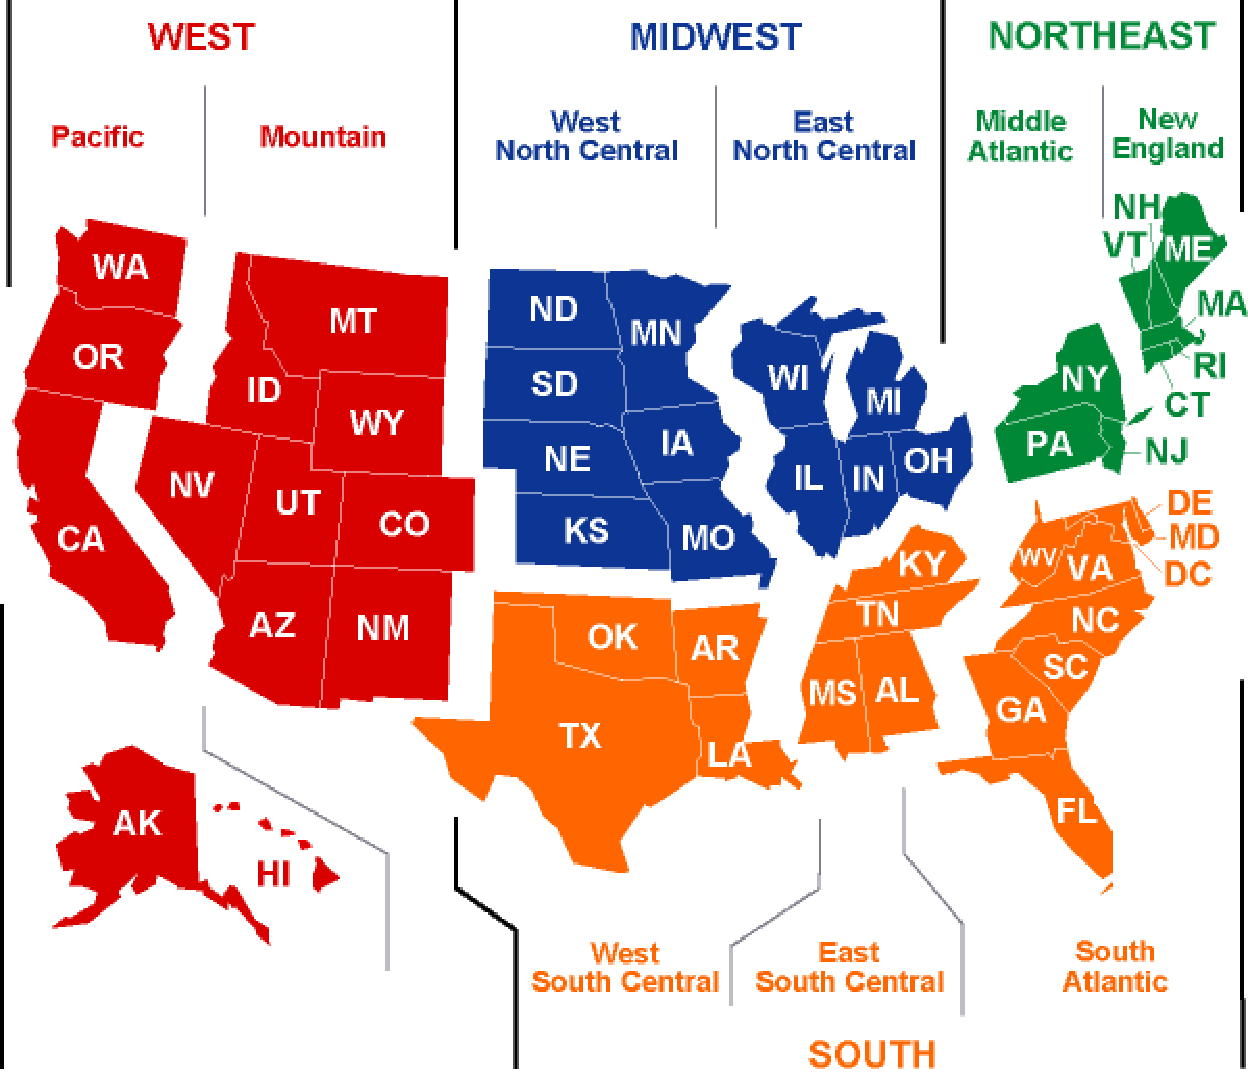
\includegraphics[height=3in]{graphsAndTables/cendivco.pdf}\centering
\caption{Census divisions.}\label{cenDiv}
\end{figure}

have a ts graph here showing happiness by division and lectricity
consumption--guess smooth them

\section{States}

This paper started as one author frequently flies from NJ to TX and noticed from
the air and on the ground huge differences in energy use between the two
states. Bigger houses, roads, cars, indeed everything is big in Texas! And
indeed differences are striking--Texas consumee about twice as much enbrgy as NJ
does per capita; yet interestingly not a big difference in residential energy
consumption--perhaps everything is newer in TX and hence more enrgy
efficent. The biggest diffences are in transportation ?? v ?? --


\begin{spacing}{.8}
{\footnotesize
\begin{verbatim}
TETPB    Total energy consumption per capita, m BTU
TERPB    Total energy consumption per capita in the residential sector, m BTU
TEAPB    Total energy consumption per capita in the transportation sector, m BTU
TECPB    Total energy consumption per capita in the commercial sector, m BTU
TEIPB    Total energy consumption per capita in the industrial sector, m BTU

sorted on TETPB, this is for 2009

. | state   TETPB   TERPB   TEAPB   TECPB   TEIPB |
  |-----------------------------------------------|
  |    RI     182      58      60      44      20 |
  |    NY     192      56      56      62      18 |
  |    HI     205      27     100      31      48 |
  |    MA     211      65      69      42      35 |
  |    CA     212      40      84      41      47 |
  |-----------------------------------------------|
  |    CT     215      71      68      52      23 |
  |    AZ     219      59      76      52      31 |
  |    FL     222      66      77      54      25 |
  |    NH     227      69      80      51      27 |
  |    NV     244      58      80      43      63 |
  |-----------------------------------------------|
  |    VT     248      80      85      47      36 |
  |    MD     256      74      81      74      27 |
  |    OR     269      68      87      51      63 |
  |    NC     273      78      76      63      56 |
  |    NJ     273      68     103      72      31 |
  |-----------------------------------------------|
  |    MI     274      76      75      61      62 |
  |    UT     274      59      86      55      74 |
  |    PA     287      73      77      54      83 |
  |    DE     294      77      79      71      67 |
  |    CO     296      68      85      60      83 |
  |-----------------------------------------------|
  |    IL     303      76      78      63      86 |
  |    GA     304      76      98      57      73 |
  |    WA     307      77      91      59      80 |
  |    VA     308      81      93      78      56 |
  |    ME     311      68      94      48     101 |
  |-----------------------------------------------|
  |    WI     313      76      76      63      98 |
  |    MO     313      89      96      69      59 |
  |    OH     321      81      82      61      98 |
  |    DC     324      61      34     222       7 |
  |    NM     325      57      99      59     110 |
  |-----------------------------------------------|
  |    ID     326      82      80      55     109 |
  |    TN     333      84      96      60      93 |
  |    MN     340      77      90      66     108 |
  |    SC     345      79      99      57     110 |
  |    AR     360      78     100      57     125 |
  |-----------------------------------------------|
  |    MS     379      75     122      54     128 |
  |    WV     382      94      92      60     136 |
  |    AL     384      78      98      54     153 |
  |    KS     402      84     102      75     141 |
  |    OK     403      80     121      65     137 |
  |-----------------------------------------------|
  |    IN     423      87      92      59     186 |
  |    NE     431      88      99      77     168 |
  |    MT     431      90     116      81     144 |
  |    KY     449      89     110      60     191 |
  |    TX     452      64     110      58     219 |
  |-----------------------------------------------|
  |    SD     453      90     113      77     173 |
  |    IA     477      81     100      68     227 |
  |    ND     656     103     133      98     321 |
  |    LA     841      79     150      62     550 |
  |    AK     904      77     273      89     465 |
  |-----------------------------------------------|
  |    WY     933      85     217     111     519 |
  +-----------------------------------------------+

(obs=306)

             |    TERPB    TEAPB    TECPB    TEIPB    TETPB
-------------+---------------------------------------------
       TERPB |   1.0000
       TEAPB |   0.2141   1.0000
       TECPB |   0.2132   0.1255   1.0000
       TEIPB |   0.3914   0.7993   0.1818   1.0000
       TETPB |   0.4418   0.8620   0.3274   0.9757   1.0000


(obs=306)

             |    TERPB    TEAPB    TECPB    TEIPB    TETPB       ls
-------------+------------------------------------------------------
       TERPB |   1.0000
       TEAPB |   0.2141   1.0000
       TECPB |   0.2132   0.1255   1.0000
       TEIPB |   0.3914   0.7993   0.1818   1.0000
       TETPB |   0.4418   0.8620   0.3274   0.9757   1.0000
          ls |   0.0952   0.2740   0.1246   0.2629   0.2839   1.0000

ls is happiness
\end{verbatim}
}
\end{spacing}

Furthermore, interestingly transportation corrlates negatively with commerce--DC
one of the most effiicnet in trasportation (61) is least efficient in commerce
(222).  Total energy consumption correlates most with transportation (.86) and
 especially industry (.9). Happiness does correlate positively with all energy
 uses, mostly with transport and industry and total (about .3). 
  

\begin{figure}[H]
 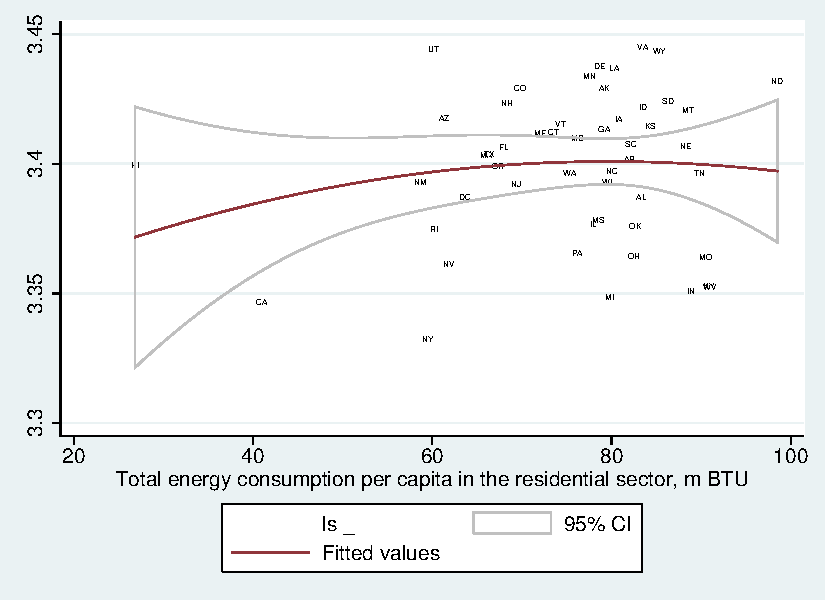
\includegraphics[height=3in]{graphsAndTables/lfTERPBls.pdf}\centering
\caption{lfTERPBls}\label{lfTERPBls}
\end{figure}

\begin{figure}[H]
 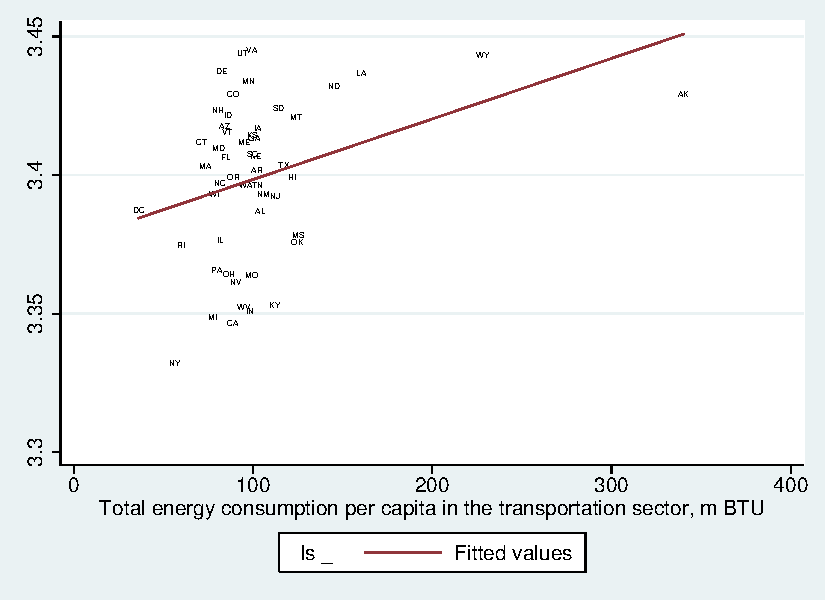
\includegraphics[height=3in]{graphsAndTables/lfTEAPBls.pdf}\centering
\caption{lfTEAPBls}\label{lfTEAPBls}
\end{figure}

\begin{figure}[H]
 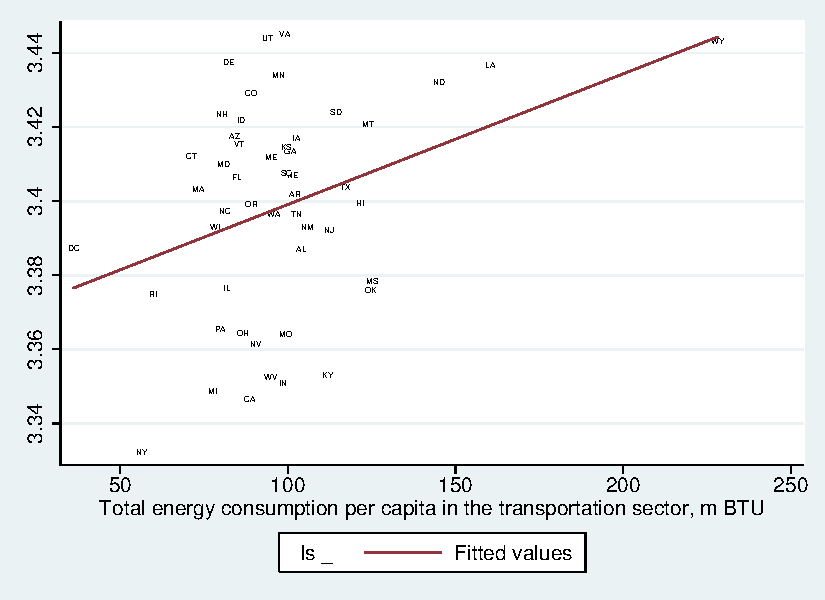
\includegraphics[height=3in]{graphsAndTables/lfTEAPBlsNoAk.pdf}\centering
\caption{no alaska; lfTEAPBlsNoAk}\label{lfTEAPBlsNoAk}
\end{figure}

\begin{figure}[H]
 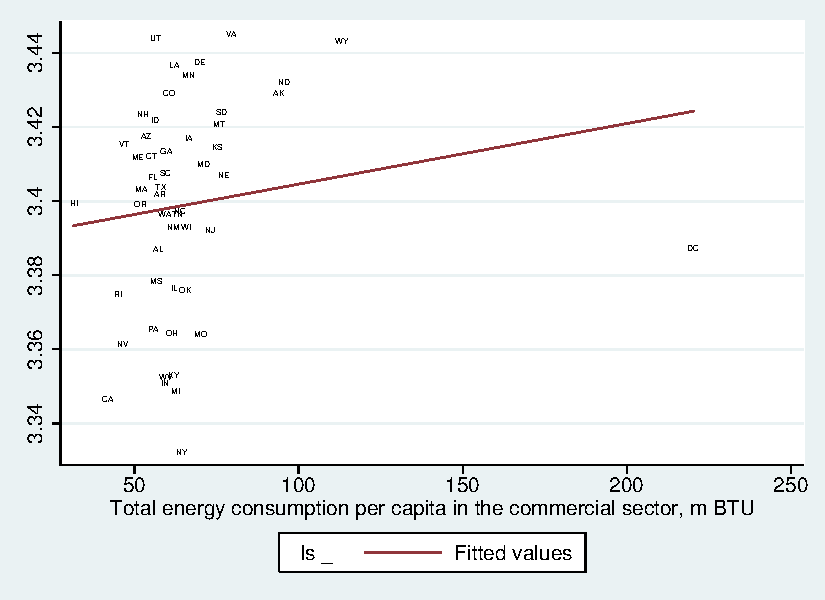
\includegraphics[height=3in]{graphsAndTables/lfTECPBls.pdf}\centering
\caption{lfTECPBls}\label{lfTECPBls}
\end{figure}

\begin{figure}[H]
 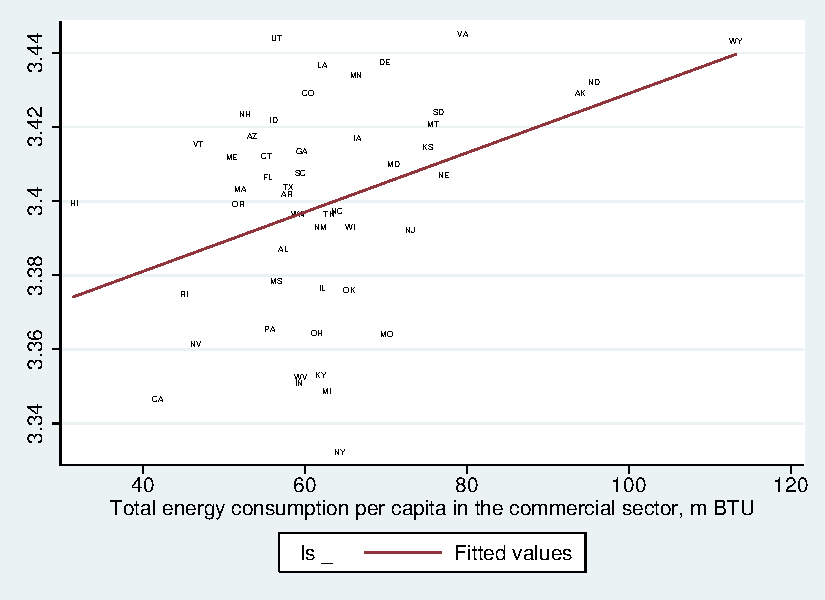
\includegraphics[height=3in]{graphsAndTables/lfTECPBlsNoDc.pdf}\centering
\caption{lfTECPBlsNoDc}\label{lfTECPBlsNoDc}
\end{figure}

\begin{figure}[H]
 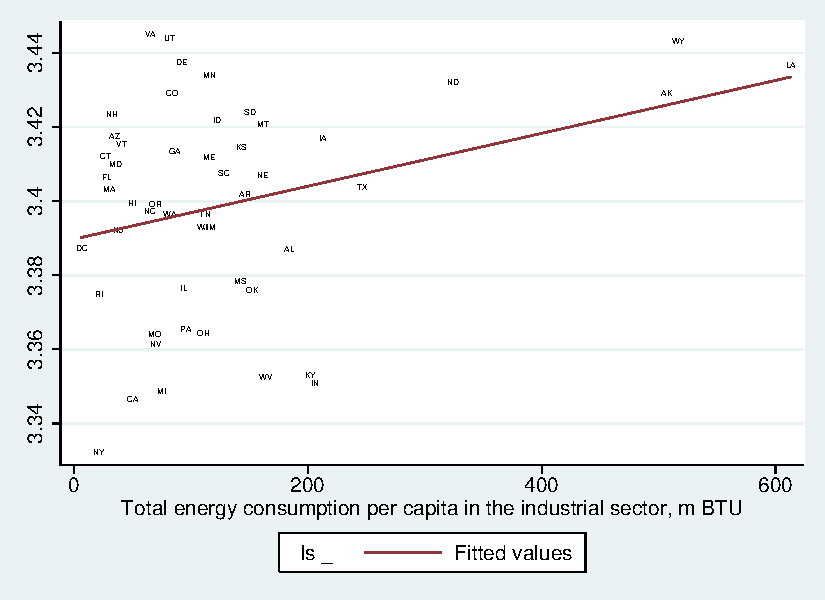
\includegraphics[height=3in]{graphsAndTables/lfTEIPBls.pdf}\centering
\caption{lfTEIPBls}\label{lfTEIPBls}
\end{figure}

\begin{figure}[H]
 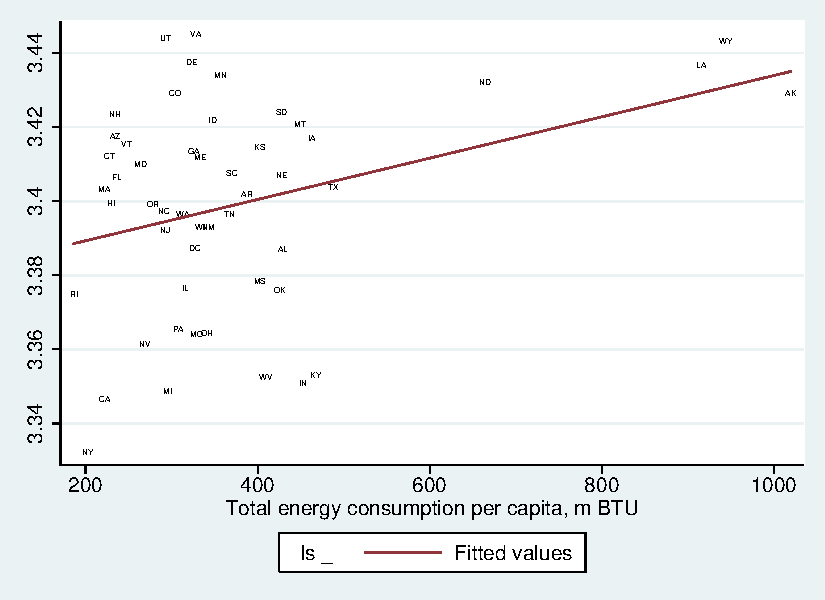
\includegraphics[height=3in]{graphsAndTables/lfTETPBls.pdf}\centering
\caption{lfTETPBls}\label{lfTETPBls}
\end{figure}


 We 
expect the  more dense and more urban areas are less happy. Note that ppulation
density and percent urban are very different variables--population density is
largely driven by history-when state was established--Western States (except
California) are less dense than North Eestern states. It is also driven by  size
of state--large states like Pennsylvania are less dense than smaller states like
Rhode Island. Percent urban is different--and it reflects administrative
prcesses such as zoning and is sensitive to a defninition of urban area. There are large differences in both
variables. In some North Eastern states there are more than 1,000 people per
square mile (NJ, RI), in most Western states, on the other hand, there are fewer
than 100 people per square mile. Several states are above 90\% urban, yet few
states are mostly non urban. Below a table sorted on population density.

Finally, we will look at 2 key variables for happiness, social support, one
measure of social capital, and the other ``harder'' measure--general
health. States in West and North are more supportive with an exception of
Delaware, which is very supportive and surrounded by unsupportive states.


\begin{spacing}{.8}
\begin{verbatim}
  | state     popDen   perUrb |  .  +---------------------+ 
  |---------------------------|     | state   supp     gh | 
  |    AK   .0012512    66.02 |     |---------------------| 
  |    WY   .0058089    64.76 |     |    HI   4.03   3.52 | 
  |    MT   .0068089    55.89 |     |    NY   4.05   3.60 | 
  |    ND    .009768     59.9 |     |    CA   4.09   3.53 | 
  |    SD   .0107636    56.65 |     |    DC   4.10   3.72 | 
  |---------------------------|     |    TX   4.11   3.46 | 
  |    NM   .0170242    77.43 |     |---------------------| 
  |    ID   .0190094    70.58 |     |    MS   4.11   3.30 | 
  |    NE   .0238206    73.13 |     |    AZ   4.13   3.57 | 
  |    NV   .0246217     94.2 |     |    CT   4.15   3.71 | 
  |    UT   .0337594    90.58 |     |    PA   4.15   3.55 | 
  |---------------------------|     |    FL   4.16   3.52 | 
  |    KS   .0349687     74.2 |     |---------------------| 
  |    OR   .0399737    81.03 |     |    MI   4.17   3.53 | 
  |    ME   .0430245    38.66 |     |    SC   4.18   3.47 | 
  |    CO   .0487062    86.15 |     |    NV   4.18   3.51 | 
  |    IA   .0546036    64.02 |     |    RI   4.19   3.64 | 
  |---------------------------|     |    IN   4.19   3.48 | 
  |    OK      .0548    66.24 |     |---------------------| 
  |    AR    .056154    56.16 |     |    KY   4.20   3.35 | 
  |    AZ   .0564202    89.81 |     |    MO   4.20   3.48 | 
  |    MS   .0632948    49.35 |     |    NM   4.21   3.51 | 
  |    MN   .0666861    73.27 |     |    AR   4.21   3.42 | 
  |---------------------------|     |    MT   4.21   3.59 | 
  |    VT   .0679205     38.9 |     |---------------------| 
  |    WV   .0771272    48.72 |     |    OH   4.21   3.51 | 
  |    MO   .0872253    70.44 |     |    IL   4.21   3.53 | 
  |    AL   .0945003    59.04 |     |    NE   4.22   3.61 | 
  |    TX   .0966383     84.7 |     |    AL   4.22   3.34 | 
  |---------------------------|     |    NH   4.22   3.69 | 
  |    WA   .1014513    84.05 |     |---------------------| 
  |    WI   .1050449    70.15 |     |    NJ   4.22   3.61 | 
  |    LA   .1051988    73.19 |     |    OR   4.23   3.58 | 
  |    KY    .110114    58.38 |     |    CO   4.23   3.69 | 
  |    NH   .1471073     60.3 |     |    NC   4.23   3.47 | 
  |---------------------------|     |    WA   4.24   3.59 | 
  |    TN   .1541655    66.39 |     |---------------------| 
  |    SC   .1542213    66.33 |     |    ME   4.24   3.60 | 
  |    GA   .1688821    75.07 |     |    SD   4.25   3.64 | 
  |    MI   .1746762    74.57 |     |    VT   4.25   3.74 | 
  |    IN   .1811528    72.44 |     |    ID   4.25   3.57 | 
  |---------------------------|     |    OK   4.25   3.38 | 
  |    NC   .1966354    66.09 |     |---------------------| 
  |    VA   .2031902    75.45 |     |    MA   4.26   3.74 | 
  |    HI   .2123741    91.93 |     |    MD   4.26   3.63 | 
  |    IL   .2312725    88.49 |     |    VA   4.27   3.63 | 
  |    CA   .2396597    94.95 |     |    LA   4.27   3.40 | 
  |---------------------------|     |    WY   4.27   3.63 | 
  |    OH   .2825454    77.92 |     |---------------------| 
  |    PA   .2840687    78.66 |     |    KS   4.27   3.60 | 
  |    FL   .3514421    91.16 |     |    GA   4.28   3.54 | 
  |    NY   .4116164    87.87 |     |    WI   4.28   3.61 | 
  |    DE   .4618843     83.3 |     |    AK   4.28   3.64 | 
  |---------------------------|     |    UT   4.29   3.71 | 
  |    MD    .596153     87.2 |     |---------------------| 
  |    CT   .7391024    87.99 |     |    IA   4.29   3.60 | 
  |    MA   .8414038    91.97 |     |    ND   4.30   3.59 | 
  |    RI   1.018562    90.73 |     |    WV   4.30   3.26 | 
  |    NJ      1.197    94.68 |     |    MN   4.31   3.72 | 
  |---------------------------|     |    DE   4.31   3.62 | 
  |    DC          .      100 |     |---------------------| 
  +---------------------------+     |    TN   4.32   3.42 | 
\end{verbatim}                      +---------------------+ 
\end{spacing}


Below regressions follow.  We have
seen that there is a weak to modearte relationshipe between energy use per
capita in different sectors and in general and happiness. How do these
relationships hold in regrressions? We proceed in a following way. We look at
three major energy uses: residential, commericial ,and transport  and also
total. We leave off indusrtial hence this energy is less liekly to impact
werllbeing of people directly and it may bias it--because this energy use is
dicatted by industry--there may be indiorect effects--thourgh employment, wages
adn development, but that shoudl be picked up by GDP. 
First, we
consider a model where we control for level of economic development (per capita
incoime). Then we add envioronmental factors, density, percent urban and avergae
temoertaures in Jan and Jul follwoning \cite{abdallah08al, brereton08}--we use
average for each month Jun and Jul and not the single max day. Finally, and this
is perhaps innovation in ecological literature, we add at state level two
aggregated from BRFSS key person level prodictors of happiness--social support
and happiness--tehre is substantail variation on these variables as discussed earlier.

We do not control for crime that is distributed unevenly within each state, and
hence global control in not informative.  

Let's start with residential energy, TERPB.
In column 1, relationship is positive  However, once controlling in column 2 for
population density and percent urban and tempoeratures , the relationship
between TERPB and happiness disappears. Likewise, when added in column 3
controls for social support and general health, the raltionship stays
non-existent. 


In transportation (TEAPB), on the other hand, the relationship is
positive, and if anything it increases with added controls, which is
puzzling. There are at least 2 explanations--perhaps thrill of travel %TODO cite
                                %from my ls_car paper  
Also, Americans prefer \cite{fuguitt90,fuguitt75} and are happier
\cite{aok_hea_spr,aok11a} in suburbs than in big cities, and there are likely
to be more consumption of energyu  in ransportatin in states woith more suburbs.
Likewise, when considering total energy use (TETPB) a positive relationship
persists. This warrants further exploration. 

\begin{table}[H]\centering \caption{ols1} \label{ols1} \begin{scriptsize} \begin{tabular}{p{1.4in}p{.43in}p{.43in}p{.43in}p{.43in}p{.43in}p{.43in}p{.43in}p{.43in}p{.43in}p{.43 in}p{.43in}p{.43 in}}\hline                     &      TERPB1   &      TERPB2   &      TERPB3   &      TEAPB1   &      TEAPB2   &      TEAPB3   &      TETPB1   &      TETPB2   &      TETPB3   \\
Total energy consumption per capita in the residential sector, m BTU&       0.000+  &       0.000   &       0.000   &               &               &               &               &               &               \\
Total energy consumption per capita in the transportation sector, m BTU&               &               &               &       0.000***&       0.000** &       0.000***&               &               &               \\
Total energy consumption per capita, m BTU&               &               &               &               &               &               &       0.000***&       0.000+  &       0.000***\\
Real gross domestic product, m chain 05usd, PC&       0.000+  &       0.002***&       0.001***&       0.000*  &       0.002***&       0.000+  &       0.000   &       0.002***&       0.000   \\
popukation density, thosands per sq m&               &      -0.029***&      -0.023***&               &      -0.022** &      -0.012** &               &      -0.024** &      -0.012*  \\
perUrb              &               &      -0.001***&      -0.001***&               &      -0.000** &      -0.000***&               &      -0.001** &      -0.000***\\
avgJanTemp          &               &      -0.000   &       0.001***&               &      -0.000   &       0.001***&               &      -0.000   &       0.001***\\
avgJulTemp          &               &       0.001*  &       0.002***&               &       0.001*  &       0.002***&               &       0.001*  &       0.002***\\
gh                 &               &               &       0.204***&               &               &       0.221***&               &               &       0.233***\\
supp               &               &               &       0.203***&               &               &       0.201***&               &               &       0.191***\\
constant            &       3.368***&       3.261***&       1.654***&       3.369***&       3.256***&       1.605***&       3.373***&       3.263***&       1.616***\\
N                   &         306   &         288   &         288   &         306   &         288   &         288   &         306   &         288   &         288   \\
 \hline\multicolumn{6}{l}{+p$<$0.10 *p$<$0.05 **p$<$0.01 ***p$<$0.001; robust standard errors} \end{tabular}\end{scriptsize}\end{table}


First considering enrgy use in residential and in commerce (columns a),
interestingly it appears that the positive relationship is driven by commerce,
residential energyu use indeed  turns negative. Then in columns b, when
considering all, three, residential, commerce, and transportation, thw first two
remain insignificant and transportation coomes out positive


\begin{table}[H]\centering \caption{ols2} \label{ols2} \begin{scriptsize} \begin{tabular}{p{1.4in}p{.43in}p{.43in}p{.43in}p{.43in}p{.43in}p{.43in}p{.43in}p{.43in}p{.43in}p{.43 in}p{.43in}p{.43 in}}\hline                     &          a1   &          a2   &          a3   &          b1   &          b2   &          b3   \\
Total energy consumption per capita in the residential sector, m BTU&       0.000   &      -0.000   &      -0.000+  &       0.000   &      -0.000   &      -0.000   \\
Total energy consumption per capita in the transportation sector, m BTU&               &               &               &       0.000***&       0.000   &       0.000***\\
TET*                &               &               &               &               &               &               \\
Total energy consumption per capita in the commercial sector, m BTU&       0.000   &       0.001***&       0.001***&      -0.000   &       0.000   &      -0.000   \\
Real gross domestic product, m chain 05usd, PC&       0.000   &       0.002***&       0.000*  &       0.000   &       0.002***&       0.000+  \\
popukation density, thosands per sq m&               &      -0.023** &      -0.018***&               &      -0.022** &      -0.012** \\
perUrb              &               &      -0.001***&      -0.001***&               &      -0.001** &      -0.000** \\
avgJanTemp          &               &      -0.000   &       0.001***&               &      -0.000   &       0.001***\\
avgJulTemp          &               &       0.001*  &       0.002***&               &       0.001*  &       0.002***\\
gh                 &               &               &       0.201***&               &               &       0.218***\\
supp               &               &               &       0.208***&               &               &       0.204***\\
constant            &       3.374***&       3.280***&       1.665***&       3.350***&       3.276***&       1.603***\\
N                   &         306   &         288   &         288   &         306   &         288   &         288   \\
 \hline\multicolumn{6}{l}{+p$<$0.10 *p$<$0.05 **p$<$0.01 ***p$<$0.001; robust standard errors} \end{tabular}\end{scriptsize}\end{table}

These findings are lagrly replicated with fixed effects estimatiion--there is no
increase in happiness from energy use in residential or total, but tehre is an
increase in transportation. Note, hausman test indicates that we should use
fixed, not random effect.  


\begin{table}[H]\centering \caption{fe1} \label{fe1} \begin{scriptsize} \begin{tabular}{p{1.4in}p{.43in}p{.43in}p{.43in}p{.43in}p{.43in}p{.43in}p{.43in}p{.43in}p{.43in}p{.43 in}p{.43in}p{.43 in}}\hline                     &      TERPB1   &      TERPB2   &      TERPB3   &      TEAPB1   &      TEAPB2   &      TEAPB3   &      TETPB1   &      TETPB2   &      TETPB3   \\
Total energy consumption per capita in the residential sector, m BTU&      -0.001+  &      -0.001   &      -0.000   &               &               &               &               &               &               \\
Total energy consumption per capita in the transportation sector, m BTU&               &               &               &      -0.000+  &      -0.000   &       0.000+  &               &               &               \\
Total energy consumption per capita, m BTU&               &               &               &               &               &               &      -0.000   &       0.000   &       0.000   \\
Real gross domestic product, m chain 05usd, PC&       0.003***&       0.003***&       0.003***&       0.003***&       0.003** &       0.002** &       0.003***&       0.002*  &       0.002** \\
popukation density, thosands per sq m&               &       0.456   &       0.027   &               &       0.532   &       0.175   &               &       0.687+  &       0.135   \\
perUrb              &               &       0.011***&       0.008** &               &       0.011***&       0.008** &               &       0.011***&       0.008** \\
avgJanTemp          &               &       0.000   &       0.000   &               &       0.000+  &       0.000   &               &       0.001*  &       0.000   \\
avgJulTemp          &               &       0.003***&       0.002***&               &       0.002***&       0.001** &               &       0.002***&       0.002***\\
gh                 &               &               &       0.212***&               &               &       0.220***&               &               &       0.212***\\
supp               &               &               &       0.162***&               &               &       0.168***&               &               &       0.161***\\
constant            &       3.307***&       2.211***&       1.168***&       3.288***&       2.193***&       1.033***&       3.285***&       2.140***&       1.134***\\
N                   &         306   &         288   &         288   &         306   &         288   &         288   &         306   &         288   &         288   \\
 \hline\multicolumn{6}{l}{+p$<$0.10 *p$<$0.05 **p$<$0.01 ***p$<$0.001; robust standard errors} \end{tabular}\end{scriptsize}\end{table}


%TODO defineitly have beta coeff some hwere--see what ecological econ
%doeas--maybe in app if they don;t do that a lot..

\section{Counties}

\begin{figure}[H]
 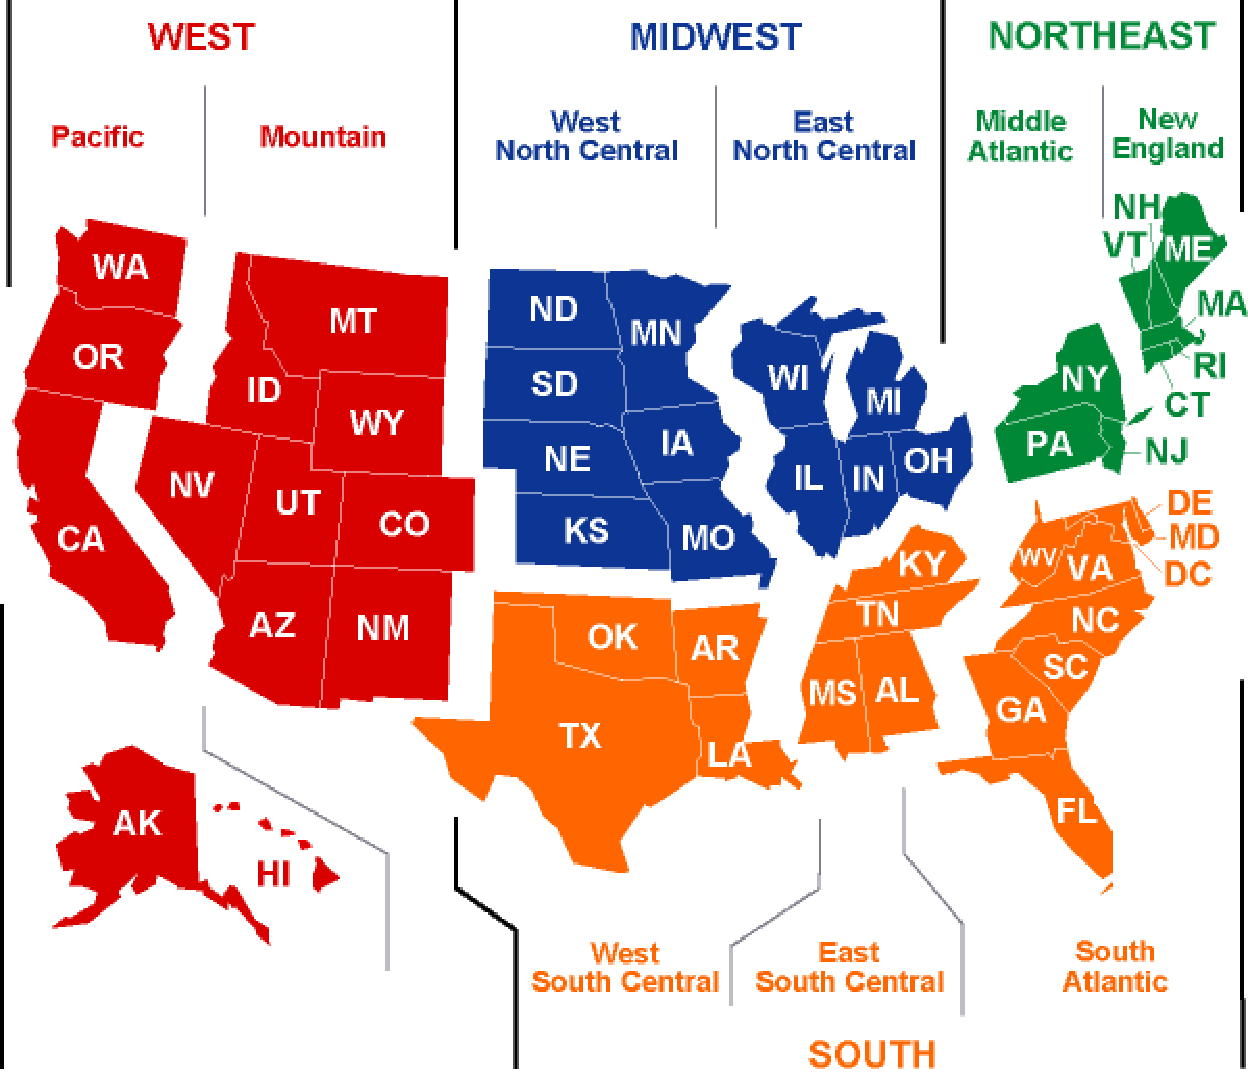
\includegraphics[height=3in]{graphsAndTables/cendivco.pdf}\centering
\caption{California climate divisions correspondencies with California
  counties. \url{http://www.cpc.ncep.noaa.gov/products/analysis_monitoring/regional_monitoring/CLIM_DIVS/california.gif}.}\label{caCD}
\end{figure}

Note, as shown in figure \ref{caCD}, there is not always an exact overlap
between counties and climate divisions. They were matched in the following way

The limitation of states is that, well, it is very ecological--large areas! and
second, there is not much difference is happijess ascross states, buit there is
much more across counties. 

Here in bivariate case, too, like across states, there is a positive
relationshipe between energy consumprion and happiness, yet it is somewhat
weaker. 

\begin{figure}[H]
 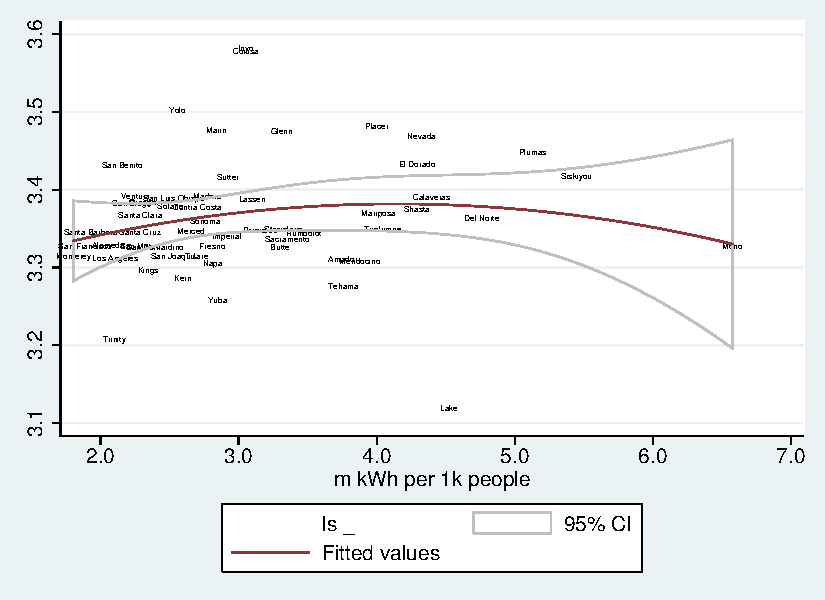
\includegraphics[height=3in]{graphsAndTables/lfELERESls.pdf}\centering
\caption{lfELERESls}\label{lfELERESls}
\end{figure}

\begin{figure}[H]
 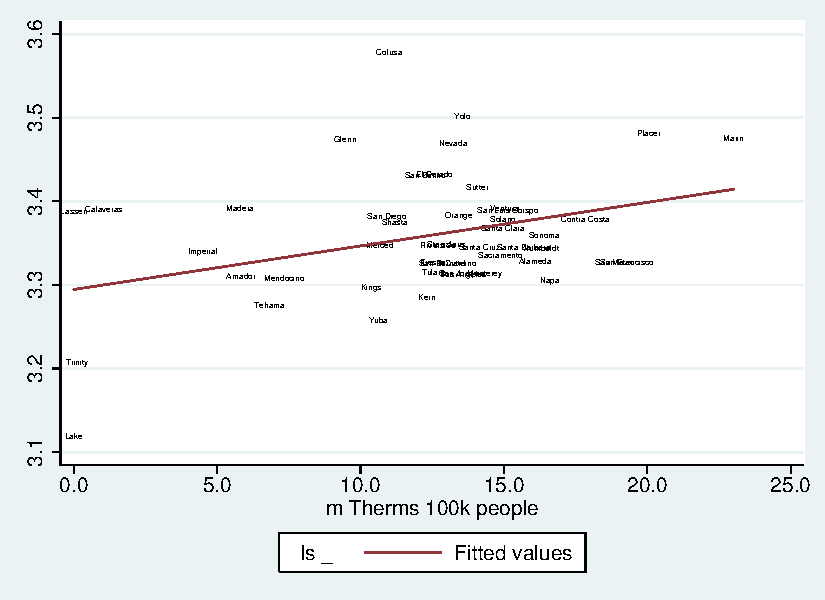
\includegraphics[height=3in]{graphsAndTables/lfGASls.pdf}\centering
\caption{lfGASls}\label{lfGASls}
\end{figure}



\begin{spacing}{.8}
\begin{verbatim}
SORTED OON ELERES
  ----------------------------------+
           county   eleres   eletot |
  ----------------------------------|
          Trinity      0.8      8.1 |
         Monterey      1.8      5.9 |
             Inyo      1.9      4.5 |
    Santa Barbara      1.9      7.5 |
    San Francisco      1.9      7.3 |
  ----------------------------------|
      Los Angeles      2.0      6.8 |
          Alameda      2.0      7.2 |
       San Benito      2.1      5.6 |
        San Diego      2.1      6.1 |
          Ventura      2.1      6.5 |
  ----------------------------------|
      Santa Clara      2.2      9.3 |
   San Bernardino      2.2      6.5 |
        San Mateo      2.3      6.6 |
            Kings      2.3      9.7 |
           Orange      2.3      6.9 |
  ----------------------------------|
       Santa Cruz      2.3      4.8 |
           Solano      2.4      7.5 |
  San Luis Obispo      2.4      6.1 |
      San Joaquin      2.4      8.1 |
             Yolo      2.5      8.2 |
  ----------------------------------|
             Kern      2.5     17.7 |
           Tulare      2.5      8.5 |
           Merced      2.6     14.1 |
     Contra Costa      2.6      8.8 |
           Madera      2.7      9.1 |
  ----------------------------------|
           Fresno      2.7      7.5 |
             Napa      2.8      7.5 |
            Marin      2.8      5.6 |
           Sonoma      2.8      5.9 |
           Sutter      2.8      6.3 |
  ----------------------------------|
             Yuba      2.8      6.7 |
        Riverside      2.8      6.2 |
         Imperial      2.8      8.0 |
           Colusa      3.0     12.0 |
           Lassen      3.0     11.5 |
  ----------------------------------|
       Stanislaus      3.2      8.9 |
       Sacramento      3.2      7.5 |
            Glenn      3.3     10.7 |
            Butte      3.3      6.5 |
         Humboldt      3.6      6.8 |
  ----------------------------------|
           Tehama      3.7      7.8 |
           Amador      3.7      8.4 |
           Placer      3.8      8.4 |
        Mendocino      3.9      6.8 |
         Mariposa      4.0      6.2 |
  ----------------------------------|
         Tuolumne      4.1      8.1 |
           Shasta      4.2      8.8 |
        El Dorado      4.2      6.9 |
           Nevada      4.3      6.7 |
        Calaveras      4.4      7.1 |
  ----------------------------------|
             Lake      4.6      7.0 |
        Del Norte      4.8      8.1 |
           Plumas      5.2     10.2 |
         Siskiyou      5.4     11.2 |
             Mono      6.6     14.5 |
  ----------------------------------|
           Alpine        .        . |
           Sierra        .        . |
            Modoc        .        . |
  				   
  ----------------------------------+

SORTED ON GASRES

           county   gasres   gastot |
  ----------------------------------|
             Lake      0.0      0.0 |
           Lassen      0.0      0.0 |
          Trinity      0.2      0.5 |
        Calaveras      1.0      2.0 |
         Imperial      4.4     17.6 |
  ----------------------------------|
           Madera      5.8     28.3 |
           Amador      5.8     24.1 |
           Tehama      6.9     17.3 |
        Mendocino      7.3     12.1 |
            Glenn      9.5     27.6 |
  ----------------------------------|
            Kings     10.2     44.9 |
           Merced     10.6     45.3 |
             Yuba     10.7     16.6 |
        San Diego     10.9     18.1 |
           Colusa     11.1    121.9 |
  ----------------------------------|
           Shasta     11.4     19.2 |
        Riverside     12.1     18.3 |
             Kern     12.1    276.3 |
       San Benito     12.2     23.7 |
           Fresno     12.3     30.3 |
  ----------------------------------|
           Tulare     12.4     35.3 |
        El Dorado     12.7     17.3 |
       Stanislaus     12.9     33.6 |
   San Bernardino     13.2     24.1 |
           Orange     13.4     21.2 |
  ----------------------------------|
           Nevada     13.4     19.1 |
            Butte     13.4     21.6 |
             Yolo     13.5     30.9 |
      San Joaquin     13.5     28.9 |
           Sutter     13.8     22.7 |
  ----------------------------------|
      Los Angeles     13.8     31.8 |
         Monterey     13.9     26.0 |
       Santa Cruz     13.9     21.9 |
      Santa Clara     14.5     25.6 |
       Sacramento     14.8     22.2 |
  ----------------------------------|
          Ventura     14.9     24.3 |
  San Luis Obispo     15.0     29.3 |
           Solano     15.1     54.6 |
    Santa Barbara     15.5     29.9 |
         Humboldt     15.7     24.7 |
  ----------------------------------|
          Alameda     15.8     27.7 |
           Sonoma     16.0     23.7 |
             Napa     16.6     29.2 |
           Placer     17.6     26.1 |
     Contra Costa     17.8     96.4 |
  ----------------------------------|
        San Mateo     18.4     30.7 |
    San Francisco     19.0     32.7 |
            Marin     22.6     31.4 |
            Modoc        .        . |
           Alpine        .        . |
  ----------------------------------|
        Del Norte        .        . |
         Siskiyou        .        . |
             Inyo        .        . |
           Plumas        .        . |
             Mono        .        . |
  ----------------------------------|
           Sierra        .        . |
         Mariposa        .        . |
         Tuolumne        .        . |
  ----------------------------------+

\end{verbatim}
\end{spacing}


And now regressions. Natural gas usage is a function of its availabily, not
necassarily gas hunger--for instance Lassen County has zero natural gas
use. Furthermore if gas is unused then it may be compensated with other sources,
hence electricty and gas in one regression. And as expected, no effect in
happiness. 

\begin{table}[H]\centering \caption{CAols1} \label{CAols1} \begin{scriptsize} \begin{tabular}{p{1.4in}p{.43in}p{.43in}p{.43in}p{.43in}p{.43in}p{.43in}p{.43in}p{.43in}p{.43in}p{.43 in}p{.43in}p{.43 in}}\hline                     &     eleres1   &     eleres2   &     eleres3   &     eletot1   &     eletot2   &     eletot3   &     gasres1   &     gasres2   &     gasres3   &     gastot1   &     gastot2   &     gastot3   \\
m kWh per 1k people &       0.020   &       0.023   &       0.009   &               &               &               &       0.041** &       0.041*  &       0.016   &               &               &               \\
per capita personal income&       0.000** &       0.000***&       0.000   &       0.000*  &       0.000** &       0.000   &       0.000   &       0.000   &      -0.000   &       0.000***&       0.000***&       0.000   \\
popDen              &               &      -0.000*  &      -0.000   &               &      -0.000** &      -0.000   &               &      -0.000+  &      -0.000   &               &      -0.000** &      -0.000   \\
avgJanTemp          &               &       0.001   &       0.002   &               &      -0.001   &       0.002   &               &       0.001   &       0.002   &               &      -0.002   &       0.002   \\
avgJulTemp          &               &       0.003   &       0.003   &               &       0.003   &       0.003   &               &      -0.000   &       0.001   &               &       0.002   &       0.001   \\
gh                 &               &               &       0.135*  &               &               &       0.146** &               &               &       0.105+  &               &               &       0.134*  \\
supp               &               &               &       0.183*  &               &               &       0.185*  &               &               &       0.194*  &               &               &       0.195*  \\
m kWh per 1k people &               &               &               &       0.001   &       0.001   &       0.002   &               &               &               &       0.007   &       0.006   &       0.005   \\
m Therms 100k people&               &               &               &               &               &               &       0.005   &       0.005   &       0.004   &               &               &               \\
m Therms 100k people&               &               &               &               &               &               &               &               &               &      -0.000   &      -0.000   &      -0.000   \\
constant            &       3.227***&       2.916***&       1.773***&       3.294***&       3.085***&       1.764***&       3.134***&       3.092***&       1.966***&       3.229***&       3.160***&       1.825***\\
N                   &         219   &         219   &         219   &         219   &         219   &         219   &         198   &         198   &         198   &         198   &         198   &         198   \\
 \hline\multicolumn{6}{l}{+p$<$0.10 *p$<$0.05 **p$<$0.01 ***p$<$0.001; robust standard errors} \end{tabular}\end{scriptsize}\end{table}


and in table \ref{CAfe1} a bit of bummer --elecricity residential appears to
have effect on happiness if in fixed effects model adn together with natural gas:(
\begin{table}[H]\centering \caption{CAfe1} \label{CAfe1} \begin{scriptsize} \begin{tabular}{p{1.4in}p{.43in}p{.43in}p{.43in}p{.43in}p{.43in}p{.43in}p{.43in}p{.43in}p{.43in}p{.43 in}p{.43in}p{.43 in}}\hline                     &     eleres1   &     eleres2   &     eleres3   &     gasres1   &     gasres2   &     gasres3   \\
m kWh per 1k people &       0.053*  &       0.062*  &       0.037   &       0.154***&       0.164***&       0.149***\\
per capita personal income&      -0.000   &       0.000   &       0.000   &      -0.000   &       0.000   &       0.000   \\
popDen              &               &      -0.000   &       0.000   &               &      -0.000   &      -0.000   \\
avgJanTemp          &               &       0.005   &       0.005   &               &       0.005   &       0.006+  \\
avgJulTemp          &               &       0.001   &       0.006   &               &      -0.001   &       0.001   \\
gh                 &               &               &       0.175** &               &               &       0.177***\\
supp               &               &               &       0.148** &               &               &       0.067   \\
m Therms 100k people&               &               &               &      -0.007   &      -0.004   &       0.005   \\
constant            &       3.363***&       2.975***&       1.322+  &       3.056***&       2.799***&       1.533*  \\
N                   &         219   &         219   &         219   &         198   &         198   &         198   \\
 \hline\multicolumn{6}{l}{+p$<$0.10 *p$<$0.05 **p$<$0.01 ***p$<$0.001; robust standard errors} \end{tabular}\end{scriptsize}\end{table}
\section{Counties--SMART version}

A limitation of BRFSS data at county level is that it is not representatoibe of
counties. And there are likely problems--for instamce Mono county increased
happiness from 2.82 in 2008 to 3.62, which is an extermely large increase and
likely due to sampling. To perform a robustness check whether these results may
 be due to sampling, we have rerun m,odels using SMART verion of data that is
 represnetative of counties

!!TODO!!  




\end{spacing}
\end{document}
